\documentclass[twoside,11pt]{article}
\usepackage{jair, theapa, rawfonts}
\usepackage{amsmath,amsfonts,amssymb,amsthm}
\usepackage[vlined,algoruled,titlenumbered,noend]{algorithm2e}
\usepackage{array}
\usepackage{epsfig,subfigure,graphicx}


\usepackage{amsmath}
\usepackage{multirow}
\usepackage{graphicx}
\usepackage{minibox}
\usepackage{tikz}
\usetikzlibrary{positioning}
\usetikzlibrary{shapes,shapes.geometric,shapes.arrows}
% Tikzstyles for decision diagrams
\tikzstyle{novertex} = [draw=none, fill=none, text centered]
\tikzstyle{nvertex} = [draw=none, text centered]

% nodes
\tikzstyle{root} = [circle, draw, text centered]
\tikzstyle{inode} = [ellipse, draw, text centered, rounded corners]
\tikzstyle{terminal} = [rectangle, draw, text centered]

% edges
\tikzstyle{high} = [draw, thick, ->]
\tikzstyle{low}  = [draw, thin, dashed, ->]

\usepackage{lscape}

\def\argmax{\operatornamewithlimits{arg\max}}
\newcommand{\casemax}{\mathrm{casemax}}
\newcommand{\MarsRover}{\textsc{Mars Rover }}
\newcommand{\casemin}{\mathrm{casemin}}
\newcommand{\UB}{\mathit{UB}}
\newcommand{\LB}{\mathit{LB}}
\newcommand{\IND}{\mathit{Ind}}
\newcommand{\CONS}{\mathit{Cons}}
\newcommand{\Root}{\mathit{Root}}
\newcommand{\Max}{\mathit{Max}}
\newcommand{\sq}{\hspace{-1mm}}
\newcommand{\sqm}{\hspace{-2mm}}
\newcommand{\true}{\mathit{true}}
\newcommand{\false}{\mathit{false}}
\newcommand{\Knapsack}{\textsc{Knapsack}}
\newcommand{\MarsRoverL}{\textsc{Mars Rover Linear }}
\newcommand{\MarsRoverNL}{\textsc{Mars Rover Nonlinear }}
\newcommand{\InventoryControl}{\textsc{Inventory Control }}
\newcommand{\WaterReservoir}{\textsc{Reservoir Management }}
\newcommand{\MultiWaterReservoir}{\textsc{Multi-Reservoir }}
\newtheorem*{example*}{Example}
\newtheorem{theorem}{Theorem}[section]
\newtheorem{corollary}{Corollary}[section]
\newtheorem{lemma}{Lemma}[section]
\newtheorem{example}[lemma]{Example}

\newenvironment{mydef}[1][Definition]{\begin{trivlist}
\item[\hskip \labelsep {\bfseries #1}]}{\end{trivlist}}

%\jairheading{1}{1993}{1-15}{6/91}{9/91}
\ShortHeadings{Exact Symbolic Solutions to MDPs}
{Zamani, Sanner}
%\firstpageno{25}


\begin{document}

\title{Exact Symbolic Dynamic Programming for Hybrid State and Action MDPs}

\author{\name Zahra Zamani \email zahra.zamani@anu.edu.au \\
       \name Scott Sanner \email ssanner@nicta.com.au \\
       \addr The Australian National University and NICTA,\\
       Canberra, ACT 0200 Australia       
}

\maketitle


\begin{abstract}
Many real-world decision-theoretic planning problems can naturally be modeled using continuous states and actions. Problems such as the multi-item Inventory problem \cite{Scarf_Karlin58} have long been solved in the operation research literature using discrete variable MDPs or approximating the optimal value for continuous domains. Other work similar to that of Gaussian control deals with general continuous domains but can not handle piecewise values on the state space. Here we propose a framework to find the first exact optimal piecewise solution for problems modeled using multi-variate continuous state and action variables.

We define a Symbolic Dynamic Programming (SDP) approach using the \emph{case} calculus which provides a closed-form solution for all DP operations (e.g. continuous maximization and integration). Solutions are provided for discrete action Hybrid (i.e. discrete and continuous) state MDPs (HMDPs) using polynomial transitions with discrete noise and arbitrary reward functions. Solutions to continuous action HMDPs with piecewise linear (or univariate quadratic), discrete noise transition and reward functions are also derived. 

Apart from the solution to general HMDPs, our other contribution is the compact representation of XADDs - a continuous variable extension of Algebraic Decision Diagrams (ADDs) - with related properties and algorithms. This allows us to empirically provide efficient results for HMDPs showing the \emph{first optimal automated solution} on various continuous domains. 
\end{abstract}

\section{Introduction}
\label{Introduction}
Many stochastic planning problems in the real-world involving resources, time or spatial configurations naturally use continuous variables in their state representation.  For example, in the \MarsRover\ problem \cite{bresina02}, a rover may move continuously while navigating and must manage bounded continuous resources of battery power and daylight time as it plans scientific discovery tasks for a set of landmarks on a given day or it  

Another example is the \InventoryControl\ problem \cite{Scarf_Karlin58} with continuous resources such as petroleum products where a business manager must decide what quantity of each item to order subject to uncertain demand, (joint) capacity constraints, and reordering costs. The \WaterReservoir\ problem \cite{reservoir}, where a utility must manage continuous reservoir water levels in continuous time to avoid underflow while maximizing electricity generation revenue.

%While all these problems are naturally modeled using discrete action hybrid (discrete and continuous) state Markov Decision Processes (DA-HMDPs) or continuous action hybrid MDPs (CA-HMDPs), there has been no prior work handling piecewise transitions. 
%more here?
Little progress has been made in the recent years in developing \emph{exact} solutions for HMDPs with multiple continuous state variables beyond the subset of HMDPs  which have an optimal \emph{hyper-rectangular piecewise linear value function} \cite{feng04,li05}. \emph{Exact} solutions to multivariate continuous state \emph{and} action settings have been limited to the control theory literature for the case of linear-quadratic Gaussian (LQG) control \cite{lqgc}. 
%i.e., minimizing a quadratic cost function subject to linear dynamics with Gaussian noise in a partially observed setting.  
However, the transition dynamics and reward (or cost) for such problems cannot be piecewise --- a crucial limitation preventing the application of such solutions to many planning and operation research (OR) problems. 
Consider the famous OR problem of \InventoryControl in \cite{Scarf_Karlin58}: 
\begin{example*} [\InventoryControl]
Inventory control problems -- how much of an
item to reorder subject to capacity constraints, demand, and optimization criteria-- date back to the 1950's with Scarf's optimal solution to the \emph{single-item capacitated inventory control} (SCIC) problem.
\emph{Multi-item joint capacitated inventory (MJCIC) control} -- with upper limits
on the total storage of all items-- has proved to be an NP-hard problem and
as a consequence, most solutions resort to some form of
approximation \cite{bitran,wusd10}; indeed, we are unaware of any 
work which claims to find an exact closed-form non-myopic
optimal policy for \emph{all} (continuous) inventory states for MJCIC 
under linear reordering costs and linear holding costs.

To further clarify we provide two example of hybrid state \InventoryControl with discrete or continuous actions.
\vspace{2mm}

\textsc{Discrete Action} \InventoryControl (\textsc{DAIC}): 
A multi-item ($K$-item) inventory consists of continuous amounts of specific items $x_i$ where $i \in [0,K]$ is the number of items and $x_i \in [0,200]$. The customer demand is a stochastic boolean variable $d$ for low or high demand levels.  The order action $a_j$ takes one of two values of $(0,200)$ where the first indicates no ordering and the second assumes maximum amount of ordering which is 200. There are linear reorder costs and also a penalty for holding items. The transition and reward functions have to be defined for each continuous item $x_i$ and action $j$.
%is this good? do I need to put transition and reward? 

%We can also consider the more general  continuous action HMDP setting to this problem: 
\vspace{2mm}
\textsc{Continuous Action}  \InventoryControl (\textsc{CAIC}):
In a more general setting to this problem, the inventory can order  any of the $i$ items $y_i \in [0,200]$ considering the stochastic customer demand. 

The transition function for the continuous variable $x_i$ and action $y_i$ is defined as: 
{%\footnotesize
\vspace{-2mm}
\begin{align}
x'_i= \begin{cases}
d  : & x_i + y_i - 150 \\
\neg d : & x_i + y_i - 50    
\end{cases} 
\end{align}
and for the discrete variable $d_i$ is:
\begin{align}
\hspace{4mm}
 \mathit{P}(d'=\mathit{true}|d,\vec{x},\vec{x'})=  \begin{cases}
d     :& 0.7\\
\neg d : & 0.3	\\
\end{cases} \label{eq:trans_inv}
\end{align}
\vspace{-2mm}}

The reward is the sum of $K$ functions $R = \sum_{i=0}^K R_i $ as below:
{\footnotesize
\begin{align}
\mathcal{R} =
\begin{cases}
\sum_{j} x_j > C &: -\infty  \\	
\sum_{j} x_j \leq C &:0\\  
\end{cases} 
+ 
\begin{cases}
\sum_{j} x'_j > C &: -\infty 	\\
\sum_{j} x'_j \leq C &: 0 	\\
\end{cases}
+
\sum_{i=0}^K \Bigg( \begin{cases}
d \wedge x_i \geq 150&: 150 - 0.1 * y_i - 0.05 * x_i \\
d \wedge x_i < 150 &:   x_i - 0.1 * y_i - 0.05 * x_i \\
\neg d \wedge x_i \geq 50 &: 50 - 0.1 * y_i - 0.05 * x_i  \\
\neg d \wedge x_i < 50 &: x_i - 0.1 * y_i - 0.05 * x_i  \\
\end{cases}\nonumber\\
+
\begin{cases}
x_i < 0 &: -\infty  \\	
x_i \geq 0 &:0\\
\end{cases} 
+ 
\begin{cases}
x'_i < 0&: -\infty  \\
x'_i \geq 0 &: 0
\end{cases} \Bigg)
\label{rew_inv}
\end{align}}
where $C$ is the total capacity for $K$ items in the inventory. The first and last cases check the safe ranges of the capacity such that the inventory capacity of each item above zero and the sum of total capacity below $C$ is desired.
%%%%%%%%%%%%%%%%%%%%%%%%%%%%%%%%%%%%%%%%%%%%%%%%%%%%%%%%%%%%%%%%%%%%%%%%%%
%\vspace{5mm}
\begin{figure}[t!]
\centering
%\subfigure{
%\hspace{-20mm}
%\vspace{-3mm}
%\includegraphics[width=1 \textwidth]{Figures2/diagrams/v2_inv2_2.pdf}
\begin{subfigure}
                \centering
                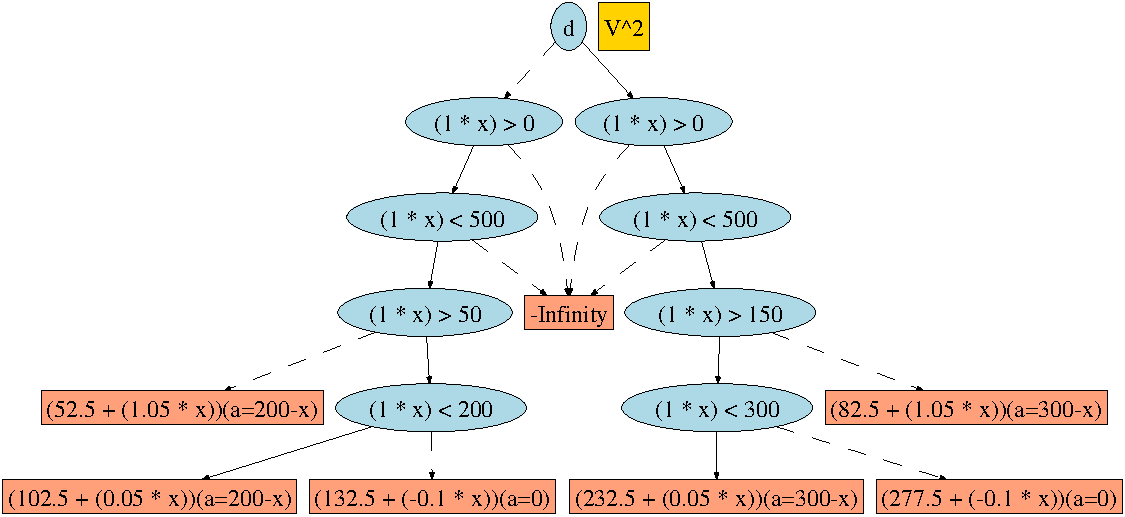
\includegraphics[width=0.68\textwidth]{pics/inv-v2.pdf}
        \end{subfigure}
                \hspace{2mm}
\begin{subfigure}
                \centering
                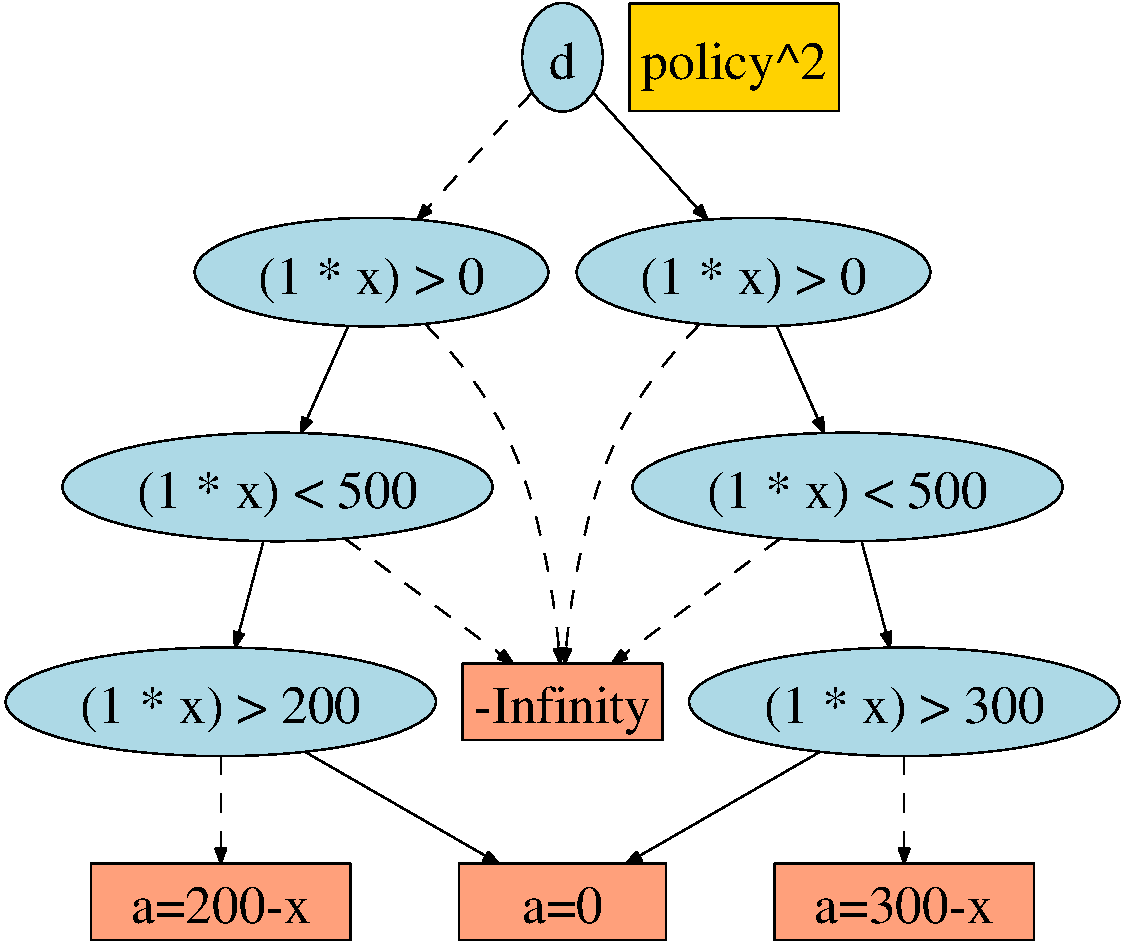
\includegraphics[width=0.26\textwidth]{pics/inv-p2.pdf}
        \end{subfigure}
\vspace{-2mm}
\caption{\footnotesize Optimal value function $V^2(x)$ for the
CAIC problem represented as an extended algebraic decision
diagram (XADD).  Here the solid lines represent the $\true$ branch for
the decision and the dashed lines the $\false$ branch.  To evaluate
$V^2(x)$ for any state $x$, one simply traverses the diagram in a
decision-tree like fashion until a leaf is reached where the
non-parenthetical expression provides the \emph{optimal value} and the
parenthetical expression provides the \emph{optimal policy} 
($a = \pi^{*,2}(x)$) to achieve value $V^2(x)$ (Left); Simplified diagram for the optimal policy for the second iteration $\pi^2$ consistent with Scarf's policy (Right).}
\label{fig:inv_policy}
\vspace{-6mm}
\end{figure}
%%%%%%%%%%%%%%%%%%%%%%%%%%%%%%%%%%%%%%%%%%%%%%%%%%%%%%%%%%%%%%%%%%%%%%%%%%
Note that illegal state values are defined using $-\infty$, in this case having the capacity lower than zero at any time and having capacity higher than that of the total $C$. 
\end{example*}

If our objective is to maximize the long-term \emph{value} $V$ (i.e. the sum of rewards received over an infinite horizon of actions), we show that the optimal value function can be derived in closed-form. 
For a single-item CAIC problem \footnote{For purposes of concise exposition and explanation
of the optimal value function and policy, this example uses
continuous univariate state and action;
the empirical results will later discuss a range of HMDPs with
multivariate hybrid state and action.}
the optimal value function for the second horizon is defined in Figure~\ref{fig:inv_policy} (left):
\vspace{-3mm}
\begin{align}
V = \begin{cases}
(x < 0 \vee x>500) &: -\infty \\
d \land (0 \leq x \leq 500) \land (x \geq 300) &:  277.5 - 0.1 * x \\
d \land (150 \leq x \leq 300) &:  232.5 + 0.05 * x \\
d \land ( 0 \leq x \leq 150) &:  82.5 + 1.05 * x \\
\neg d \land (200 \leq x \leq 500)  &:  132.5 - 0.1 * x \\
\neg d \land (50 \leq x \leq 200) &: 102.5 + 0.05 * x \\
\neg d \land (0 \leq x \leq 50) &:  52.5 + 1.05 * x \\
\end{cases} 
\label{eq:vfun_inv}
%\vspace{-7mm}
\end{align}
The policy obtained from this piecewise and linear value function and $V^2$ itself are shown in Figure~\ref{fig:inv_policy} using an extended algebraic decision diagram (XADD) representation which allows efficient implementation of the \emph{case calculus} for arbitrary functions. According to Scarf's policy for the \InventoryControl problem, if the holding and storage costs are linear the optimal policy in each horizon is always of $(S,s)$ ~\cite{Scarf_Karlin58}. In general this means if ($x>s$) the policy should be not to order any items and if ($x<s$) then ordering $S-s-x$ items is optimal. 
%%%%%%%%%%%%%%%%%%%%%%%%%%%%%%%%%%%%
According to this we can rewrite Scarf's policy where each slice of the state space matches with this general rule: 
\begin{align}
\pi^{*,2}(x) = 
\begin{cases}
(x < 0 \vee x>500) &: -\infty \\
d \land (300 \leq x \leq 500)  &:  0 \\
d \land (0 \leq x \leq 300) &:  300 - x \\
\neg d \land (200 \leq x \leq 500) &:  0 \\
\neg d \land (0 \leq x \leq 200) &:  200 - x \\
\end{cases}\nonumber
\end{align}

While this simple example illustrates the power of using continuous variables, for a multi-variate problem it is the very \textit{first solution} to exactly solving problems such as the DAIC and CAIC. 
We propose novel ideas to work around some of the expressiveness limitations of previous approaches, significantly generalizing the range of HMDPs that can be solved exactly.  To achieve this more general solution, this
paper contributes a number of important advances:
\begin{itemize}
\item The use of case calculus allows us to perform Symbolic dynamic programming (SDP) \cite{fomdp} used to solve MDPs with
piecewise transitions and reward functions defined in first-order logic. We define all required operations for SDP such as $\oplus,\ominus,max,min$ as well as new operations such as the continuous maximization of an action parameter $y$ defined as $max_y$ and integration of discrete noisy transition.
\item We perform value iteration for two different settings. In the first setting of DA-HMDP we consider continuous state variables with a discrete action set while in the second setting CA-HMDP we consider continuous states and actions. Both DA-HMDPs and CA-HMDPs are evaluated on various problem domains. The results show that DA-HMDPs applies to a wide range of transition and reward functions providing hyper-rectangular value functions. CA-HMDPs have more restriction in modeling due to the increased complexity caused by continuous actions, and limit solutions to linear and quadratic transitions and rewards but provide strong results for many problems never solved exactly before. 
\item While the \emph{case} representation for the optimal \textsc{CAIC} 
solution shown in \eqref{eq:vfun_inv} is sufficient in theory to
represent the optimal value functions that our HMDP solution
produces, this representation is unreasonable to maintain in practice
since the number of case partitions may grow exponentially on
each receding horizon control step.  For \emph{discrete} factored
MDPs, algebraic decision diagrams (ADDs) \cite{bahar93add} have been
successfully used in exact algorithms like SPUDD \cite{spudd} to
maintain compact value representations.  Motivated by this work we
introduce extended ADDs (XADDs) to compactly represent general
piecewise functions and show how to perform efficient operations on
them \emph{including} symbolic maximization.  Also we present all properties and algorithms required for XADDs. 
\end{itemize}

Aided by these algorithmic and data structure advances, we empirically demonstrate that our SDP approach with XADDs can exactly solve a variety of HMDPs with discrete and continuous actions. 


\section{Hybrid MDPs (HMDPs)}
The mathematical framework of Markov Decision Processes (MDPs) is used for modelling many stochastic sequential decision making problems ~\cite{bellman}. This discrete-time stochastic control process chooses an action $a$ available at state $s$. The process then transitions to the next state $s'$ according to $\mathcal{T}(s,s')$ and receives a reward $\mathcal{R}(s,a)$. The transition function follows the Markov property allowing each state to only depend on its previous state.  We provide novel exact solutions using the MDP framework for discrete and continuous variables in the state and action space. Hybrid state and action MDPs (HMDPs) are introduced in the next section followed by the finite-horizon solution via dynamic programming ~\cite{li05}.
%\vspace*{-0.05in}
\subsection{Factored Representation}
\label{sec:HMDPs}
%\vspace*{-0.05in}
The formal definition of a hybrid MDP (HMDP) is presented in the following: 
\begin{itemize}
\item States are represented by vectors of variables $(\vec{b},\vec{x}) = ( b_1,\ldots,b_n,x_{1},\ldots,x_m )$.  We assume
that each $b_i \in \{ 0,1 \}$ ($1 \leq i \leq m$) is boolean$\,$ and each $x_j \in \mathbb{R}$ ($1 \leq j \leq
n$) is continuous.

\item A finite set of $p$ actions $A = \{a_{1}(\vec{y}_1), \ldots, a_{p}(\vec{y}_p)\}$, where each action $a_k(\vec{y_k})$ ($1
\leq k \leq p$)  with parameter $\vec{y}_k \in \mathbb{R}^{|\vec{y}_k|}$  denotes continuous parameters for 
action $a_{k}$ and  if $|\vec{y}_k|=0$ then action $a_{k}$ has no parameters and is a discrete action.

\item The state transition model $\mathit{P}(\vec{b}',\vec{x}'|\vec{b},\vec{x},a,\vec{y})$, which specifies the
probability of the next state $(\vec{b}',\vec{x}')$ conditioned on a
subset of the previous and next state and action $a$ with its possible parameters $\vec{y}$; 

\item Reward function $\mathcal{R}(\vec{b},\vec{x},\vec{b}',\vec{x}',a,\vec{y})$, which specifies the immediate reward obtained by taking action $a(\vec{y})$ in state $(\vec{b},\vec{x})$; 

\item Discount factor $\gamma, \; 0 \leq \gamma \leq 1$.
\footnote{If time is explicitly included as one of the
continuous state variables, $\gamma = 1$ is typically used, unless
discounting by horizon (different from the state variable time) is
still intended.}  
\end{itemize}

A policy $\pi$ specifies the action $a(\vec{y}) =\pi(\vec{b},\vec{x})$ to take in each state $(\vec{b},\vec{x})$.  Our
goal is to find an optimal sequence of finite horizon-dependent
policies
%put footnote back in
\footnote{We assume a finite horizon $H$ in this
paper, however in cases where our SDP algorithm converges
in finite time, the resulting value function and 
corresponding policy are optimal for $H=\infty$. 
For finitely bounded value
with $\gamma = 1$, the forthcoming SDP algorithm may terminate in
finite time, but is not guaranteed to do so; for $\gamma < 1$, an
$\epsilon$-optimal policy for arbitrary $\epsilon$ can be computed by
SDP in finite time.
} 
$\Pi^* = (\pi^{*,1},\ldots,\pi^{*,H})$ that
maximizes the expected sum of discounted rewards over a horizon $h \in H; H \geq 0$:
\begin{align}
V^{\Pi^*}(\vec{x}) & = E_{\Pi^*} \left[ \sum_{h=0}^{H} \gamma^h \cdot r^h \Big| \vec{b}_0,\vec{x}_0 \right]. \label{eq:vfun_def}
\end{align}
Here $r^h$ is the reward obtained at horizon $h$ following $\Pi^*$ where 
we assume starting state $(\vec{b}_0,\vec{x}_0)$ at $h=0$.

 %%%%%%%%%%%%%%%%%%%%%%%%%%%%%%%%%%%%%%%%%%%%%%%%%%%%%%%%%%%%%%%%%%%%%%%%%%
%\vspace{10mm}
\begin{figure}[t!]
%\centering
%\subfigure{
%\hspace{-20mm}
%\vspace{-6mm}
 \begin{subfigure}
                \centering
                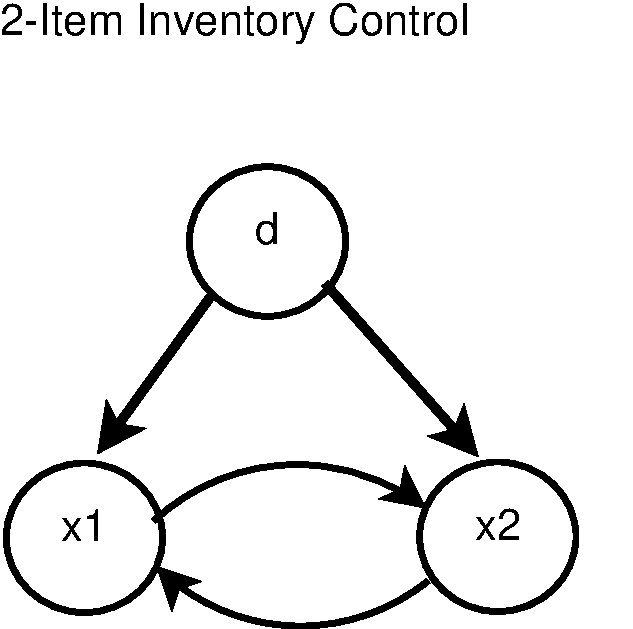
\includegraphics[width=0.2\textwidth]{pics/dbn_state.pdf}
        \end{subfigure}
                \hspace{2mm}
\begin{subfigure}
                \centering
                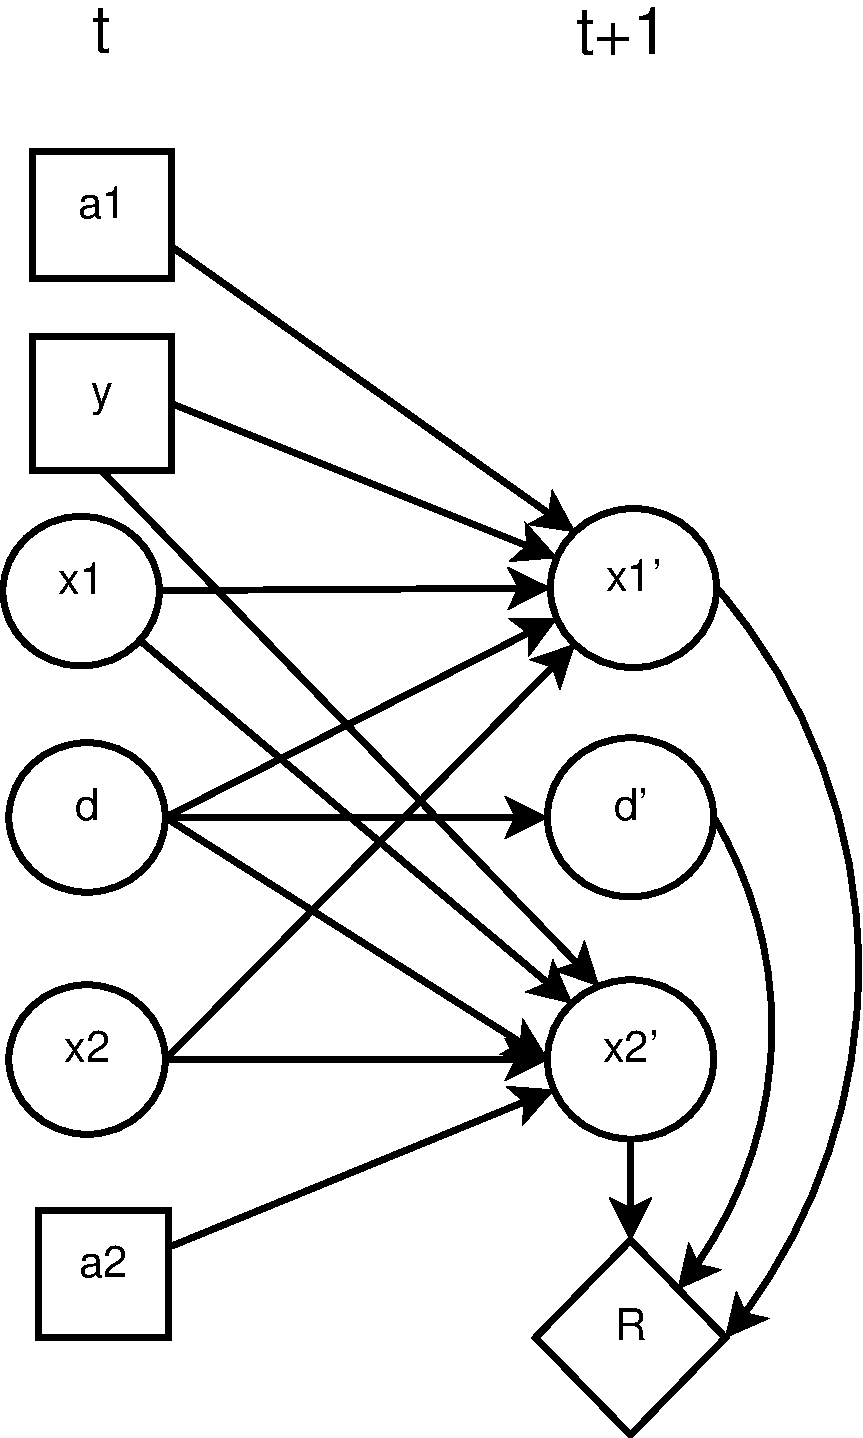
\includegraphics[width=0.22\textwidth]{pics/dbn_inv2.pdf}
        \end{subfigure}
                        \hspace{-1mm}
\begin{subfigure}
                \centering
                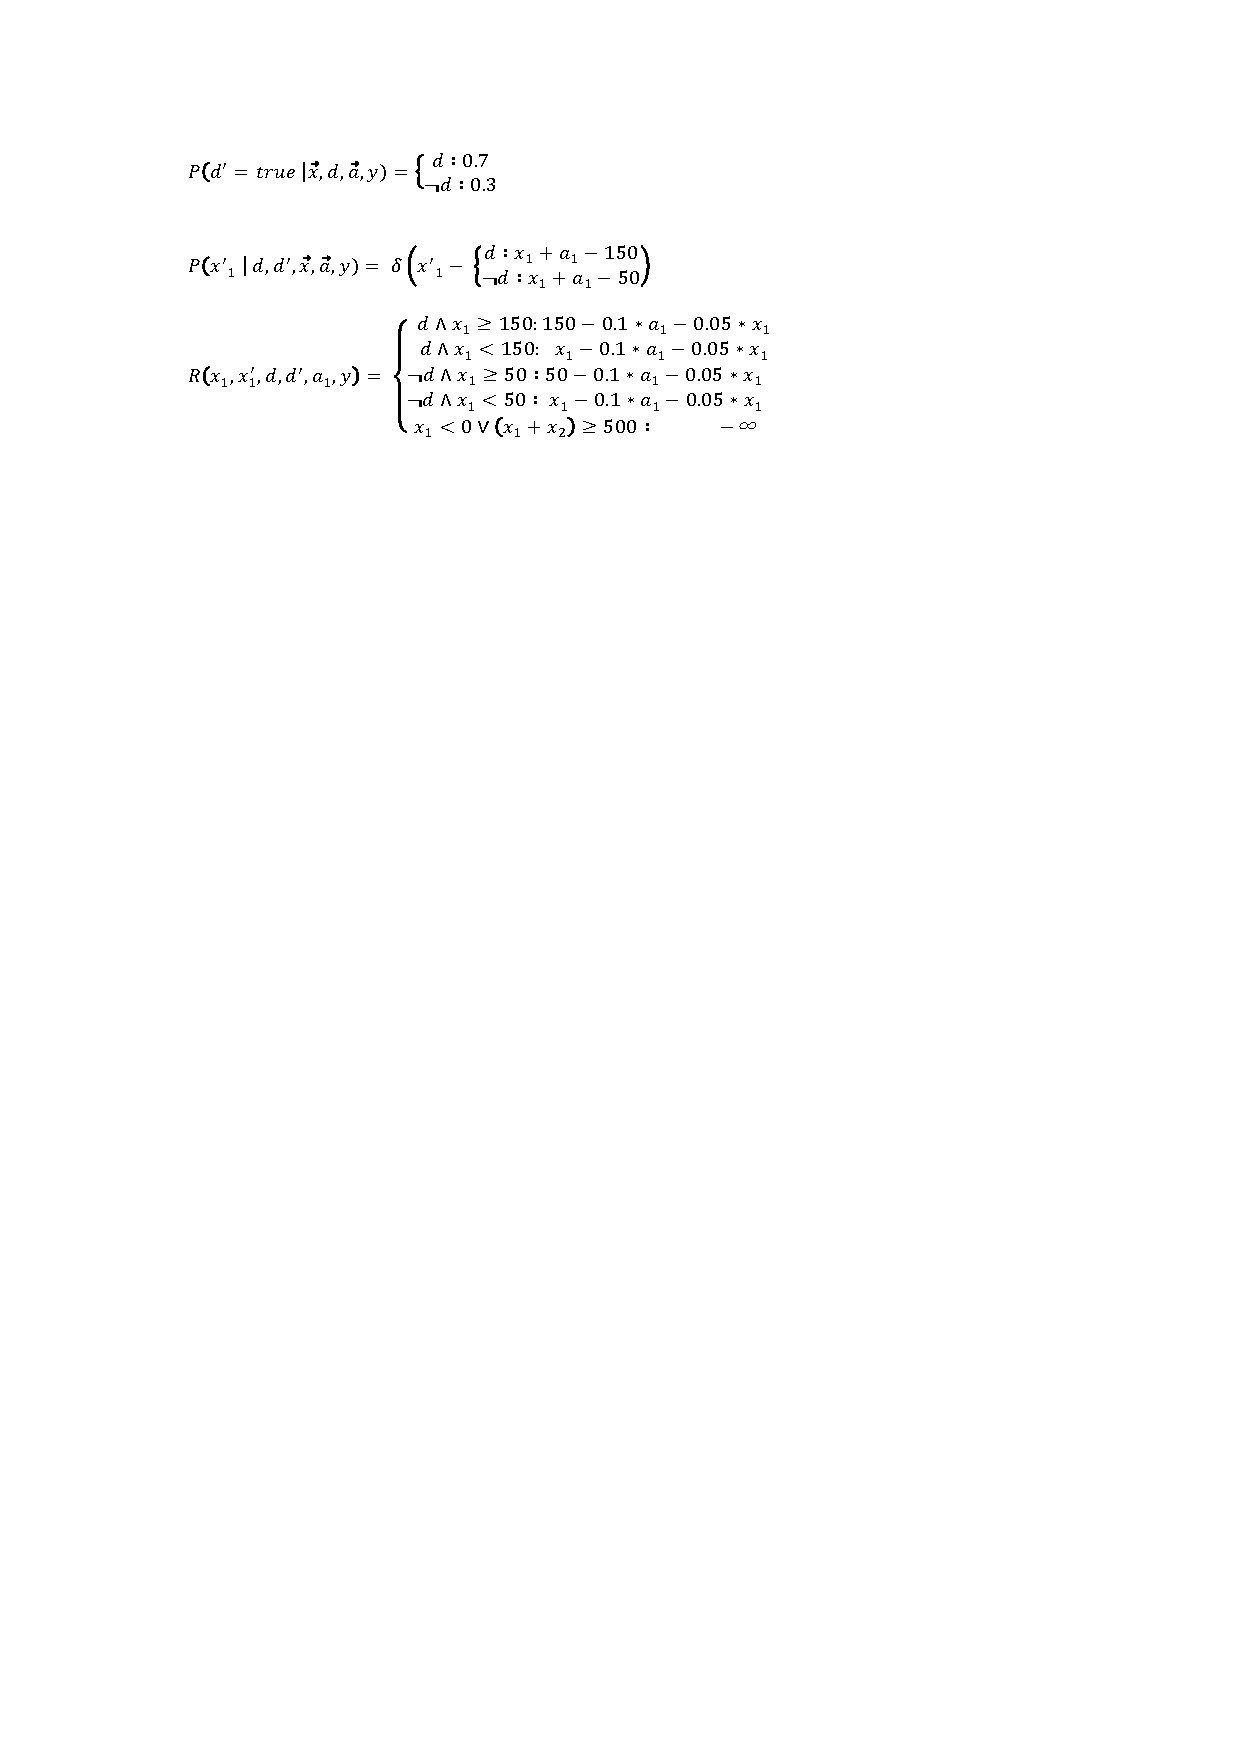
\includegraphics[width=0.52\textwidth]{pics/probabilities_2.pdf}
        \end{subfigure}
       % \vspace{-3mm}
\caption{%\footnotesize 
{\it (left)} Network topology between state variables in the 2-item continuous action \InventoryControl (CAIC) problem; {\it (middle)} DBN structure representing the transition and reward function; {\it (right)} transition probabilities and reward function in terms of CPF and PLE for $x_1$. }
\label{fig:dbn}
%\vspace{-3mm}
\end{figure}
%%%%%%%%%%%%%%%%%%%%%%%%%%%%%%%%%%%%%%%%%%%%%%%%%%%%%%%%%%%%%%%%%%%%%%%%%%

Such HMDPs are naturally factored \cite{boutilier99dt}
in terms of state variables $(\vec{b},\vec{x},\vec{y})$ where potentially $\vec{y} =0$. The transition structure can be exploited in the form of a dynamic Bayes
net (DBN) \cite{dbn} where the conditional probabilities
$P(b_i'|\cdots)$ and $P(x_j'|\cdots)$ for each next state variable can
condition on the action, current and next state. 
We can also have \emph{synchronic arcs} (variables that condition on each
other in the same time slice) within the binary $\vec{b}$ or
continuous variables $\vec{x}$ and from $\vec{b}$ to $\vec{x}$.%\footnote{Synchronic arcs between variables within $\vec{b}$ or within $\vec{x}$ can be accommodated if the forthcoming Algorithm~\ref{alg:regress} (\texttt{Regress}) is modified to multiply and marginalize-out multiple next-state variables in one elimination step according to the DBN structure.}  
Hence we can factorize the joint transition model as
{%\footnotesize
\begin{equation}
P(\vec{b}',\vec{x}'|\vec{b},\vec{x},a,\vec{y}) = 
\prod_{i=1}^n P(b_i'|\vec{b},\vec{x},\vec{b'},\vec{x'},a,\vec{y}) \prod_{j=1}^m P(x_j'|\vec{b},\vec{b}',\vec{x},\vec{x'},a,\vec{y}). \nonumber 
\end{equation}}
where $P(b_i'|\vec{b},\vec{x},\vec{b'},\vec{x'},a,\vec{y})$ may condition on a subset of
$\vec{b}$ and $\vec{x}$ in the current and next state and likewise 
$P(x_j'|\vec{b},\vec{b}',\vec{x},\vec{x'},a,\vec{y})$ may condition on a subset of
$\vec{b}$, $\vec{b}'$, $\vec{x}$ and $\vec{x'}$. Figure~\ref{fig:dbn} presents the DBN for a 2-item CAIC example according to this definition.  

We call the conditional probabilities
$P(b_i'|\vec{b},\vec{x},\vec{b'},\vec{x'},a,\vec{y})$ for \emph{binary} variables $b_i$
($1 \leq i \leq n$) conditional probability functions (CPFs) --- not
tabular enumerations --- because in general these functions can
condition on both discrete and continuous state as
in the right-hand side of~\eqref{eq:trans_inv}.  For the \emph{continuous} variables
$x_j$ ($1 \leq j \leq m$), we represent the CPFs
$P(x_j'|\vec{b},\vec{b'},\vec{x},\vec{x'},a,\vec{y})$ with \emph{piecewise
linear equations} (PLEs) satisfying the following properties: 
\begin{itemize}
\item PLEs can only condition on the action, current state, and previous state variables
\item PLEs are deterministic meaning that to be represented by probabilities they
must be encoded using Dirac $\delta[\cdot]$ functions (example forthcoming)
\item PLEs are piecewise linear, where the piecewise conditions may be arbitrary logical combinations of $\vec{b}$, $\vec{b}'$ 
and linear inequalities over $\vec{x}$ and $\vec{x'}$.  
\end{itemize}

The transition function example provided in the left-hand side of~\eqref{eq:trans_inv} can be expressed in PLE format such as the right figure in Figure~\ref{fig:dbn}:
\begin{align*}
P(x'_1 | d, d',\vec{x},\vec{a}, y) = \delta \Bigg( x'_1 -  \begin{cases}
d  : & x_i + y_i - 150 \\
\neg d : & x_i + y_i - 50    
\end{cases} \Bigg) 
\end{align*}
The use of the $\delta[\cdot]$ function ensures that the PLEs are conditional
probability functions that integrates to 1 over $x'_j$; In more intuitive
terms, one can see that this $\delta[\cdot]$ is a simple way to encode
the PLE transition $x' = \left\{ \ldots \right.$ in the form of 
$P(x_j'|\vec{b},\vec{b'},\vec{x},\vec{x'},a,\vec{y})$.

%qualify the extent of stochasticity and other restrictions
While it will be clear that our restrictions do not permit general stochastic transition noise (e.g., Gaussian noise as in LQG control), they do permit discrete noise in the sense that
$P(x_j'|\vec{b},\vec{b'},\vec{x},\vec{x'},a,\vec{y})$ may condition on
$\vec{b'}$, which are stochastically sampled according to their CPFs.
\footnote{Continuous stochastic noise for the transition function is an on going work which allows us to model stochasticity more generally}
We note that this representation effectively allows modeling of
continuous variable transitions as a mixture of $\delta$ functions,
which has been used frequently in previous exact continuous state MDP
solutions \cite{feng04,hao09}.
% should I put this????
Furthermore, we note that our
DA-HMDPs representation is more general than \cite{feng04,li05,hao09} in that
we do not restrict the equations to be linear, but rather
allow it to specify \emph{arbitrary} functions (e.g., nonlinear). 

The reward function in DA-HMDPs is defined as \emph{arbitrary} function of the current state for each action $a \in A$. 
While  empirical examples throughout the paper will demonstrate the full expressiveness of our symbolic dynamic programming approach, we note that there are computational advantages to be had when the reward and transition case conditions and functions can be restricted to linear expressions.  

Due to the same restrictions, for CA-HMDPs the reward function $R(\vec{b},\vec{b'},\vec{x},\vec{x'}, a,\vec{y})$ is defined as either of the following:

(i) a general piecewise linear function (boolean or linear conditions and linear values) as in equation~\eqref{rew_inv}; or

(ii) a piecewise quadratic function of univariate state and a linear function of univariate action parameters:
\begin{align}
R(x,x',d,d', a) & = \begin{cases}
\neg d \land x \geq -2 \land x \leq 2 : & 4 - x^2 \\
d \lor x < -2 \lor x > 2 : & 0
\end{cases} \nonumber 
\end{align}
%The reward function in a DA-HMDPs can potentially be defined as an \emph{arbitrary} function but to ensure computationally efficient results we assume piecewise linear boundaries that can be checked for consistency using a linear constraint feasibility checker, which we will later see is crucial for efficiency.

These transition and reward constraints will ensure that all derived functions in the solution of HMDPs adhere to the reward 
constraints.

%\vspace*{-0.05in}
\subsection{Solution methods}
\label{sec:soln}
Now we provide a continuous state generalization of {\it value
iteration} \cite{bellman}, which is a dynamic programming algorithm
for constructing optimal policies.  It proceeds by constructing a
series of $h$-stages-to-go value functions $V^h(\vec{b},\vec{x})$.
Initializing $V^0(\vec{b},\vec{x}) = 0$ we define the quality
$Q_a^{h}(\vec{b},\vec{x},\vec{y})$ of taking action $a(\vec{y})$ in state
$(\vec{b},\vec{x})$ and acting so as to obtain
$V^{h-1}(\vec{b},\vec{x})$ thereafter as the following:

\vspace{-4mm}
{%\footnotesize
\begin{align}
Q_a^{h}(\vec{b},\vec{x},\vec{y}) & = 
 \sum_{\vec{b}'} \hspace{-1.0mm} \int \hspace{-1.0mm} \left( \prod_{i=1}^n P(b_i'|\vec{b},\vec{b'},\vec{x},\vec{x'},a,\vec{y}) \prod_{j=1}^m P(x_j'|\vec{b},\vec{b}',\vec{x},\vec{x'},a,\vec{y}) \right) \label{eq:qfun} \\ 
& \Bigg[ R(\vec{b},\vec{b'},\vec{x},\vec{x'}, a,\vec{y}) + \gamma \cdot V^{h-1}(\vec{b}',\vec{x}') d\vec{x}'  \hspace{-0.2mm} \Bigg] \nonumber
\end{align}}
Given $Q_a^h(\vec{b},\vec{x},\vec{y})$ for each $a \in A$ where $\vec{y}$ can also be empty , we can proceed
to define the $h$-stages-to-go value function as follows:
\begin{align}
V^{h}(\vec{b},\vec{x}) & = \max_{a \in A} \max_{\vec{y} \in \mathbb{R}^{|\vec{y}|}} \left\{ Q^{h}_a(\vec{b},\vec{x},\vec{y}) \right\} \label{eq:vfun}
\end{align}

For discrete actions, maximization over the continuous parameter $\vec{y}$ is omitted. The $max_{\vec{y}}$ operator defined in the next section is required to generalize solutions from DA-HMDPs to CA-HMDPs.
If the horizon $H$ is finite, then the optimal value function is
obtained by computing $V^H(\vec{b},\vec{x})$ and the optimal
horizon-dependent policy $\pi^{*,h}$ at each stage $h$ can be easily
determined via $\pi^{*,h}(\vec{b},\vec{x}) = \argmax_a
\argmax_{\vec{y}} Q^h_a(\vec{b},\vec{x},\vec{y})$.  If the horizon $H
= \infty$ and the optimal policy has finitely bounded value, then
value iteration can terminate at horizon $h$ if $V^{h} = V^{h-1}$;
then $V^\infty = V^h$ and $\pi^{*,\infty} = \pi^{*,h}$.

In DA-HMDPs, we can always compute the value function in tabular form;
however, how to compute this for HMDPs with reward and transition
function as previously defined is the objective of the symbolic
dynamic programming algorithm that we define in the next section.

\section{Symbolic Dynamic Programming} \label{SDP}
As the name suggests, symbolic dynamic programming (SDP) \cite{fomdp}
is simply the process of performing dynamic programming (in this case
value iteration) via symbolic manipulation. Specifically, SDP provides symbolic abstraction of all functions which allows building distinct logical partitions on the state space to represent the policy and value function. While SDP as defined
in \cite{fomdp} was only used with piecewise
constant functions, in this work we generalize the representation to solve HMDPs with
general piecewise functions. Using the \emph{mathematical} definitions of the previous section, we  
show how to \emph{compute} equations~\eqref{eq:qfun} and \eqref{eq:vfun} 
symbolically.
%Should all this be taken out?
%We present the general SDP framework for value iteration in DA-HMDPs in Algorithm~\ref{alg:vi} (\texttt{VI}). Further we define  Algorithm~\ref{alg:contMax}(\texttt{Continuous Maximization}) to deal with the final maximization in (~\ref{eq:vfun}) for continuous actions.

Before we define our solution, however, we must formally define our
case representation and symbolic case operators.

\subsection{Case Representation}
\label{sec:caserep}
The case representation presented in this section allows an expressive representation of general piecewise functions. Using such case representation we can extend the SDP framework in \cite{fomdp}, which addresses only piecewise constant functions. This representation .

\begin{mydef}(\textbf{Case representation}): 
\label{defCase}
A piecewise function in a case partition notation is given by:
{%\footnotesize 
\begin{align*}
f = 
\begin{cases}
  \phi_1: & f_1 \\ 
 \vdots&\vdots\\ 
  \phi_k: & f_k, \\ 
\end{cases}
\end{align*}
}
where, $\phi_i: f_i$ is a case partition; $\phi_i$ is a logical formula and $f_i$ can be defined as an arbitrary function. The formula $\phi_i$ is defined by arbitrary logical operations ($\land,\lor,\neg$ over: 
(I) boolean variables in $\vec{b}$ and (II) 
inequalities ($\geq,>,\leq,<$) involving continuous variables $\vec{x}$. 
Each $\phi_i$ is disjoint from the other $\phi_j$ ($j \neq i$). 

However the $\phi_i$ may not exhaustively cover the state space, i.e., $f$ may only be a partial function and undefined for some variable assignments. 
However, in this work, we assume $f_i$ to be either linear or univariate quadratic on $\vec{x}$. Similarly we assume $\phi_i$ is defined over linear inequalities.
\end{mydef}

The following example is a simple function in this case form: 
\begin{align*}
f_1 = 
\begin{cases}
b \wedge (x_1+x_2 >5) : & x_1+3 \\ 
\neg b \wedge (x_1+x_2 \leq 5) : & x_1+x_2 \\ 
\end{cases} 
\end{align*}

Note that any function $f$ can be represented by a case partition notation where all $\phi_i$ are conjunctions, i.e., if $f=\{\phi: f_1$ and $\phi= \alpha_1 \vee \alpha_2$, then:

\begin{align*}
f =\{ \phi:f_1 =
\begin{cases}
  \alpha_1: & f_1 \\ 
  \alpha_2: & f_1, \\ 
\end{cases}
\end{align*}




In the next section, the main case operations required to perform SDP are presented. Note that if $f$ is continuous then all SDP operations preserve this continuous property. 

\subsection{Binary operations}
\label{BinaryOp}
For the binary operations of cross-sum $\oplus$, cross-product $\otimes$ or cross-minus $\ominus$ on two case statements, the cross-product
of the logical partitions of each case statement  $\phi_i$ and $\psi_j$ is used to perform the
corresponding operation:

{%\footnotesize 
\begin{center}
\begin{tabular}{r c c c l}
&
\hspace{-6mm} 
  $\begin{cases}
    \phi_1: & f_1 \\ 
    \phi_2: & f_2 \\ 
  \end{cases}$
$\oplus$
&
\hspace{-4mm}
  $\begin{cases}
    \psi_1: & g_1 \\ 
    \psi_2: & g_2 \\ 
  \end{cases}$
&
\hspace{-2mm} 
$ = $
&
\hspace{-2mm}
  $\begin{cases}
  \phi_1 \wedge \psi_1: & f_1 + g_1 \\ 
  \phi_1 \wedge \psi_2: & f_1 + g_2 \\ 
  \phi_2 \wedge \psi_1: & f_2 + g_1 \\ 
  \phi_2 \wedge \psi_2: & f_2 + g_2 \\ 
  \end{cases}$
\end{tabular}
\vspace{4mm}
\hspace{-2mm}

\hspace{-2mm}
\begin{tabular}{r c c c l}
&
\hspace{-6mm} 
  $\begin{cases}
    \phi_1: & f_1 \\ 
    \phi_2: & f_2 \\ 
  \end{cases}$
$\otimes$
&
\hspace{-4mm}
  $\begin{cases}
    \psi_1: & g_1 \\ 
    \psi_2: & g_2 \\ 
  \end{cases}$
&
\hspace{-2mm} 
$ = $
&
\hspace{-2mm}
  $\begin{cases}
  \phi_1 \wedge \psi_1: & f_1 \cdot g_1 \\ 
  \phi_1 \wedge \psi_2: & f_1 \cdot g_2 \\ 
  \phi_2 \wedge \psi_1: & f_2 \cdot g_1 \\ 
  \phi_2 \wedge \psi_2: & f_2 \cdot g_2 \\ 
  \end{cases}$
\end{tabular}
\vspace{4mm}
\hspace{-2mm}

\hspace{-2mm}
\begin{tabular}{r c c c l}
&
\hspace{-6mm} 
  $\begin{cases}
    \phi_1: & f_1 \\ 
    \phi_2: & f_2 \\ 
  \end{cases}$
$\ominus$
&
\hspace{-4mm}
  $\begin{cases}
    \psi_1: & g_1 \\ 
    \psi_2: & g_2 \\ 
  \end{cases}$
&
\hspace{-2mm} 
$ = $
&
\hspace{-2mm}
  $\begin{cases}
  \phi_1 \wedge \psi_1: & f_1 - g_1 \\ 
  \phi_1 \wedge \psi_2: & f_1 - g_2 \\ 
  \phi_2 \wedge \psi_1: & f_2 - g_1 \\ 
  \phi_2 \wedge \psi_2: & f_2 - g_2 \\ 
  \end{cases}$
\end{tabular}
\vspace{4mm}
\hspace{-2mm}
\end{center}
}
Some partitions resulting from
these operators may be inconsistent, that is $\phi_i \wedge \psi_j \models \perp$. In this case such a partition is discarded since it is irrelevant to the function value.

As in Section~\ref{sec:caserep} for CA-HMDPs, the functions $f_i$ and $g_i$ are restricted to be linear or univariate quadratic in the continuous parameters. While $\oplus$ and $\ominus$ preserve this property (i.e. remain closed-form), for $\otimes$ the result could exceed the second order polynomial if either $f_i$ or $g_i$ are quadratic. In such cases we may only assume the other function is piecewise constant. Conveniently, as we show in the SDP algorithm presented next, the cross-product only occurs for the multiplication of piecewise constants in piecewise linear or quadratic functions. Therefore it is safe to claim that all the binary operations defined above are closed-form.


\subsubsection*{Symbolic discrete maximization}
For SDP, we also need to perform maximization over actions for~\eqref{eq:vfun} which is fairly straightforward
to define:
%\vspace{-5mm}

{%\footnotesize
\begin{center}
\begin{tabular}{r c c c l}
&
\hspace{-9mm} $\casemax \Bigg(
  \begin{cases}
    \phi_1: & f_1 \\ 
    \phi_2: & f_2 \\ 
  \end{cases}$
$,$
&
\hspace{-4mm}
  $\begin{cases}
    \psi_1: & g_1 \\ 
    \psi_2: & g_2 \\ 
  \end{cases} \Bigg)$
&
\hspace{-4mm} 
$ = $
&
\hspace{-4mm}
  $\begin{cases}
  \phi_1 \wedge \psi_1 \wedge f_1 > g_1    : & f_1 \\ 
  \phi_1 \wedge \psi_1 \wedge f_1 \leq g_1 : & g_1 \\ 
  \phi_1 \wedge \psi_2 \wedge f_1 > g_2    : & f_1 \\ 
  \phi_1 \wedge \psi_2 \wedge f_1 \leq g_2 : & g_2 \\ 
  \phi_2 \wedge \psi_1 \wedge f_2 > g_1    : & f_2 \\ 
  \phi_2 \wedge \psi_1 \wedge f_2 \leq g_1 : & g_1 \\ 
  \phi_2 \wedge \psi_2 \wedge f_2 > g_2    : & f_2 \\ 
  \phi_2 \wedge \psi_2 \wedge f_2 \leq g_2 : & g_2 \\ 
  \end{cases}$\label{symbolicMax}
\end{tabular}
\end{center}
}

For CA-HMDPs, if all $f_i$ and $g_i$ are linear, the $\casemax$ result is clearly still linear. If the $f_i$ or $g_i$ are quadratic with univariate variables (i.e. no bilinear terms such as $x_1x_2$), the expressions $f_i > g_i$ or $f_i \leq
g_i$ will be at most univariate quadratic. Any such constraint
can then be \emph{linearized} into a combination of at most 
two linear inequalities (unless tautologous or inconsistent) 
by completing the square (e.g., 
%$x^2 + 8x > 0 \equiv [x + 4]^2 > 4 \equiv [x \leq -2] \lor [x > 6]$
$-x^2 + 20x - 96 > 0 \equiv [x - 10]^2 \leq 4 \equiv [x > 8] \land [x \leq 12]$).  Hence
the result of this $\casemax$
operator will be representable in the restricted case format assumed in this paper
(i.e. linear inequalities in decisions). 

The key observation here is the case statements are closed under the binary operation of continuous case maximization (or minimization). Additionally while it may seem that this operation leads to a blowup in the number of case partitions, the XADDs presented in the next section can exploit the internal structure of the continuous case maximization to represent it more compactly. 

Furthermore, the 
XADD that we introduce later will be able to exploit the 
internal decision structure of this
maximization to represent it much more compactly.
\subsection{Unary Operations}

% TODO: adicionar um paragrafo para início da seção
\subsubsection{Scalar multiplication and Negation}
Scalar multiplication $c\cdot f$ (for
a constant $c \in \mathbb{R}$) and negation $-f$ on case statements are applied to each case partition
$f_i$ ($1 \leq i \leq k$) as follows:
{%\footnotesize
\begin{center}
\begin{tabular}{r c c l}
&
%\hspace{5mm}
  $c \cdot f = \begin{cases}
    \phi_1  : & c \cdot f_1 \\ 
   \vdots&\vdots\\ 
    \phi_k : & c \cdot f_k \\ 
  \end{cases}$
 &
\hspace{10mm}
  $-f = \begin{cases}
    \phi_1 : & - f_1 \\ 
   \vdots&\vdots\\ 
    \phi_k : & - f_k \\ 
  \end{cases}$
\end{tabular}
\end{center}
}

\subsubsection{Restriction}
In restriction $f|_{\phi}$ %is fairly simple: in this operation, 
we want to restrict a function $f$ to apply only in cases
that satisfy some formula $\phi$.  
By appending $\phi$ to each case partition we make sure that all partitions must satisfy $\phi$:

{%\footnotesize
\begin{center}
\begin{tabular}{r c c l}
&
\hspace{-6mm} 
  $f = \begin{cases}
    \phi_1: & f_1 \\ 
   \vdots&\vdots\\ 
    \phi_k: & f_k \\ 
  \end{cases}$
&

&
\hspace{-2mm}
  $f|_{\phi} = \begin{cases}
    \phi_1 \land \phi : & f_1 \\ 
   \vdots&\vdots\\ 
    \phi_k \land \phi : & f_k \\ 
  \end{cases}$
\end{tabular}
\end{center}
}
Since $f|_{\phi}$ only applies when $\phi$ holds and is
undefined otherwise, $f|_{\phi}$ is partial unless $\phi \equiv \top$.

\subsubsection{Substitution}
Symbolic substitution takes
a set $\sigma$ of variables and their substitutions and applies it to function $f$. 
Consider $\sigma = \{ x_1' / (x_1 \hspace{-.8mm} + \hspace{-.8mm} x_2), x_2' / x_1^2 \hspace{-.3mm} \exp(x_2) \}$
where the left-hand side of $/$ represents the substitution variable and the
right-hand side of $/$ represents the expression that should be substituted in its place.  
The substitution of a non-case function $f_i$ with $\sigma$ 
is $f_i\sigma$. If
$f_i = x_1' + x_2'$ then using the $\sigma$ defined above we obtain $f_i\sigma = x_1 + x_2 + x_1^2 \exp(x_2)$.  

Substitution into case partitions $\phi_j$ is performed 
by applying $\sigma$ to each inequality operand, i.e.:
\begin{align}
\begin{tabular}{r c c l}
\hspace{-2mm}
  $f\sigma = \begin{cases}
    \phi_1\sigma: & f_1\sigma \\ 
   \vdots&\vdots\\ 
    \phi_k\sigma: & f_k\sigma \\ 
  \end{cases}$
\end{tabular}
\label{SubEq}
\end{align}

Note that if $f$ has mutually exclusive partitions $\phi_i$ ($1 \leq i \leq k$)
then $f\sigma$ must also have mutually exclusive partitions. 
This is followed from the logical consequence that 
if $\phi_1 \land \phi_2 \models \bot$
then $\phi_1\sigma \land \phi_2\sigma \models \bot$.

Consider the following example with the $\sigma$ given above and $f$ given by: 
\begin{align*}
f &= \begin{cases}
 x_1' \leq \exp(x_2'): & x_1' + x_2' \\ 
 x_1' \geq \exp(x_2'): & x_1'^2 - 3x_2' \\ 
\end{cases}
\end{align*}
then $f \sigma$ is as follows:
\begin{align*}
f \sigma &= \begin{cases}
 x_1 + x_2 \leq \exp(x_1^2 \exp(x_2)): & x_1 + x_2 + x_1^2 \exp(x_2) \\ 
 x_1 + x_2 \geq \exp(x_1^2 \exp(x_2)): & (x_1 + x_2)^2 - 3x_1^2 \exp(x_2) \\ 
\end{cases}
\end{align*}


\subsubsection{Marginalization of Continuous Variables}
\label{MargContVar}
Marginalization of a continuous variable $x_j$ is performed by the integral
$\int_{x_j= - \infty}^{\infty} f(x_j) P(x_j) d x_j$. As mentioned before, we assume the probabilities of continuous variables are encoded using Direc $\delta$ functions. Thus, the integral becomes 
 $\int_{x_j= - \infty}^{\infty} f(x_j)\delta[x_j - h(\vec{z})]$, where $h(\vec{z})$ can be defined as a case statement and $\vec{z}$ does not contain $x_j$. This integral triggers the substitution $\sigma = \{ x_j / h(\vec{z}) \}$ on $f$, that is
\begin{align}
\int_{x_j =-\infty}^{\infty} f(x_j)
\delta\left[ x_j - \begin{cases}
    \phi_1: & h_1 \\ 
   \vdots&\vdots\\ 
    \phi_k: & h_k \\ 
  \end{cases} \right] dx_j =% f(x_j) \{ x_j / h(\vec{z}) \}   = 
  \begin{cases}
    \phi_1: & f \{ x_j / h_1 \} \\ 
   \vdots&\vdots\\ 
    \phi_k: & f \{ x_j/ h_k \}  \\ 
  \end{cases}. \label{eq:gen_int}
\end{align}

As an example consider marginalizing $x_1'$ in the function:

\begin{align*}
f (x_1',x_1,x_2)&= \begin{cases}
    x'_1 \geq 5 : & x'_1 + x_2 \\ 
    x'_1 < 5: & x_1 \\ 
  \end{cases} 
\end{align*}
with the transition probability function $\delta\left[ x_1' - (2x_1 + x_2) \right]$. 

The result of marginalization is: 
\begin{align*}
f (x_1',x_1,x_2)&= \begin{cases}
    x'_1 \geq 5 : & x'_1 + x_2 \\ 
    x'_1 < 5: & x_1 \\ 
  \end{cases} 
 \\
 \int_{x_1'} f(x_1',x_1,x_2)\delta\left[ x_1'- (2x_1+x_2) \right] dx_1'&= \begin{cases}
   2x_1 + x_2 - 5 \geq 0 : & 2x_1 + 2x_2 \\ 
    2x_1 + x_2 -5  < 0 : & x_1 \\
  \end{cases}
  \end{align*}
 
For a generic $\delta$ function with multiple case partitions, each of the $f$ partitions are replaced into the multiple partitions of $\delta$. Such nested case statements are then reduced back down to a standard case
statement using a simple approach:

\begin{align*}
    \begin{cases}
      \phi_1: & 
        \begin{cases}
          \psi_1: & f_{11} \\ 
          \psi_2: & f_{12}  \\ 
        \end{cases} \\
      \phi_2: & 
        \begin{cases}
          \psi_1: & f_{21} \\ 
          \psi_2: & f_{22}  \\ 
        \end{cases} \\
    \end{cases} & \; = \;
        \begin{cases}
          \phi_1 \land \psi_1: & f_{11} \\ 
          \phi_1 \land \psi_2: & f_{12}  \\ 
          \phi_2 \land \psi_1: & f_{21} \\ 
          \phi_2 \land \psi_2: & f_{22}  \\ 
        \end{cases} 
\end{align*}

%As For SDP operations, this integration is defined as $\int_{x_j'} f(x_j')\mathit{P}(x_j'|\cdots) dx_j'$ where $P(x_j'|\cdots)$
%is in the form $\delta[x_j' - h(\vec{z})]$.
%\footnote{As we see in subsequent , probabilities must be encoded using Dirac $\delta[\cdot]$ functions to ensure that a conditional probability function integrates to 1 over $x_j'$}
 
\subsubsection{Symbolic Continuous Maximization}
\label{contmax}
\emph{Continuous Maximization} of a function w.r.t $\vec{y}$ is defined as $g(\vec{b},\vec{x}) := \max_{\vec{y}}
\, f(\vec{b},\vec{x},\vec{y})$ where we crucially note that 
\emph{the} maximizing $\vec{y}$ is a function of $(\vec{b},\vec{x})$, i.e., $h(\vec{b},\vec{x}) := \argmax_{\vec{y}} \, f(\vec{b},\vec{x},\vec{y})$, thus the maximization is a \emph{symbolic} 
constrained optimization.

Exploiting the commutativity of $\max$, we can first rewrite any multivariate $\max_{\vec{y}}$ as a sequence of univariate $\max$ operations 
$\max_{y_1} \cdots \max_{y_{\textit{lenght}(\vec{y})}}$, i.e., 
$$\max_{\vec{y}}= \max_{y_{\textit{lenght}(\vec{y})}} (\cdots (\max_{y_2}(\max_{y_1}));$$ hence is suffices to provide just the univariate $\max_{y}$ solution: $g(\vec{b},\vec{x}) := \max_{y}
\, f(\vec{b},\vec{x},y)$.

Also, as a consequence of the mutual disjointness of the case partitions in $f$, we can rewrite $f(\vec{b},\vec{x},y)$ as: \footnote{The second line ensures that all illegal values are mapped to $-\infty$.}

{%\footnotesize
\begin{center}
\begin{tabular}{r c c l}
&
\hspace{-6mm} 
  $f = \begin{cases}
    \phi_1: & f_1 \\ 
   \vdots&\vdots\\ 
    \phi_k: & f_k \\ 
  \end{cases}$
&
\hspace{-2mm}
  $ =  \casemax \left[  \begin{cases}
    \phi_1: & f_1 \\
    \neg \phi_1: & -\infty \\    
  \end{cases}, 
  \cdots ,
  \begin{cases}
    \phi_k: & f_k \\
    \neg \phi_k: & -\infty \\    
  \end{cases}   
  \right]$
  \hspace{-2mm}
  $ = \casemax_{i=1,\cdots,k}\begin{cases}
    \phi_i: & f_i \\
    \neg \phi_i: & -\infty \\    
  \end{cases}$
  
\end{tabular}
\end{center}
}
where $\casemax_{i=1,\cdots,k}$ denotes $\casemax$ for $1\leq i \leq k$; and since we have $\casemax(F, -\infty) = F$, a partition 
$ \begin{cases}
    \phi_i: & f_i \\
    \neg \phi_i: & -\infty \\    
  \end{cases}$ can be represented only by the case partition $\phi_i : f_i$.   

Finally, we use these transformations to compute the $\max_y f(\vec{b},\vec{x},y)$ as follows:

\begin{align}
\max_y f(\vec{b},\vec{x},y) & = 
\max_y \casemax_{i=1,\cdots,k} \, 
\phi_i(\vec{b},\vec{x},y) : f_i(\vec{b},\vec{x},y). \nonumber \\
\end{align} 

Because 
$\max_y$ and $\casemax_i$ are commutative, i.e, can be reordered,
we compute $\max_y$ for \emph{each case partition
individually} as:  

\begin{align}
g(\vec{b},\vec{x}) = \max_y f(\vec{b},\vec{x},y)& = \casemax_i \, \fbox{$\max_y 
\phi_i(\vec{b},\vec{x},y) : f_i(\vec{b},\vec{x},y).$} \label{eq:casemax_max}
\end{align} 


\paragraph{Maximum of a single case partition.} We can now show how to (symbolically) compute the maximum for a single case partition 
$\max_y \phi_i(\vec{b},\vec{x},y): f_i(\vec{b},\vec{x},y)$.

We know that the maximum of a continuous function $f_i$ must occur at the critical points of the function --- 
either the upper or lower bounds ($\UB$ and $\LB$) of $y$, 
or in the quadratic case, in the $\Root$ (i.e., zero) of $\frac{\partial}{\partial y} f_i$.  Notice that each of $\UB$, $\LB$, and $\Root$
is a symbolic function of $\vec{b}$ and $\vec{x}$. 

We observe that each constraint of the conjunction \footnote{As we have mentioned in the case representation definition (Section \ref{sec:caserep}), we can assume without loss of generality that partitions are only conjuntions.} $\phi_i$ serves one of
purposes: 
\begin{itemize}
\item if the constraint is of the kind
$y < \alpha$ or $y \leq \alpha$ then 
$\alpha \in$ \emph{upper bound ($\UB$) on $y$};
\item if the constraint is of the kind
$y >\alpha$ or $y \geq \alpha$ then
$\alpha \in$ \emph{lower bound ($\LB$) on $y$}
\footnote{For purposes of evaluating
a case function $f$ at an upper or lower bound,
it does not matter whether a bound is inclusive ($\leq$ or $\geq$)
or exclusive ($<$ or $>$) since $f$ is required to be continuous
and hence evaluating at the limit of the inclusive bound will
match the evaluation for the exclusive bound.};
\item if the constraints do not contain $y$
and can be safely factored outside of the $\max_y$ then it belongs to an \emph{independent set ($\IND$)}. 
\end{itemize}

Note that there can be multiple symbolic upper and lower
bounds on $y$, thus in general we will need to determine the highest lower bound ($HLB$) and the lowest upper bound ($LUB$): 
$$HLB = \casemax(\alpha_j), \forall \alpha_j \in \LB$$  $$LUB = \casemin(\alpha_j), \forall \alpha_j \in \UB$$.

Given the \emph{potential} maximal points of $f$, $y = LUB$, $y = HLB$, and
$y = \Root$ of $\frac{\partial}{\partial y} f_i(\vec{b},\vec{x},y)$
w.r.t. constraints $\phi_i(\vec{b},\vec{x},y)$ --- which are all
symbolic functions --- we must symbolically evaluate which yields the
maximizing value $\Max$ for this case partition:
\vspace{2mm}
{%\footnotesize
\begin{align}
\Max =  \sq \begin{cases}
\mbox{$\exists \Root\ and\ HLB \leq \Root \leq LUB$}  \sq: \sq & \sqm \casemax( f_i \{ y / \Root \}, f_i \{ y / LUB \}, f_i \{ y / HLB \})\\
\mbox{elseif}\ HLB \leq LUB \sq:  \sq & \sqm \casemax( f_i \{ y / LUB \}, f_i \{ y / HLB \})
\end{cases}
\label{eq:maxhlblub}
\end{align}}
The 
substitution operator $\{ y / f \}$ replaces $y$ with case statement $f$, as we have previously defined. Additional constraints arise from the
symbolic nature of the $LUB$, $HLB$, and $\Root$. Specifically, we need to ensure that indeed $HLB \leq \Root \leq LUB$
(or if no root exists, then $HLB \leq LUB$)

At this point, we have almost completed the computation
of the $\max_y \phi_i(\vec{b},\vec{x},y) f_i(\vec{b},\vec{x},y)$
except for two issues: (i) the incorporation of the independent ($\IND$) constraints
(factored out previously). 
%by building a set
%of constraints $\CONS$ that ensure these conditions hold; to do this,
%it suffices to ensure that for each possible expression $\alpha$ used to
%construct $\LB$ that $\alpha \leq \Root$ and similarly for the $Root$ and $\UB$.
Finally, we express the final result as a single case partition:
\begin{equation}
\max_y \phi_i(\vec{b},\vec{x},y) f_i(\vec{b},\vec{x},y) \;\; = \;\;
  \IND: \Max .
\label{eq:maxcasepartition}
\end{equation}
Hence, to complete the maximization for an entire case statement $f$, we need only apply the above procedure to each case partition of $f$ and then perform a symbolic $\casemax$ on all of the results. In the next section we will illustrate these operations using the \InventoryControl example.  

\subsection{Symbolic Value Iteration (SVI)}
\label{section:SVI}
%%%%%%%%%%%%%%%%%%%%%%%%%%%%%%%%%%%%%%%%%%%%%%%%%%%%%%%%%%%%%%%%%%%%%%%%
\incmargin{.5em}
\linesnumbered
\begin{algorithm}[t!]
%\vspace{-.5mm}
\dontprintsemicolon
\SetKwFunction{regress}{\sc Regress}
\SetKwFunction{contmax}{\sc ContinuousMaximization}
\Begin
{
   $V^0 \leftarrow 0, h\leftarrow 0$\;
   \While{$h < H$}
   {
       $h\leftarrow h+1$\;
       \ForEach {$a(\vec{y}) \in A$}
       {
              $Q_a^{h}(\vec{y})\,\leftarrow \,$\regress{$HMDP, V^{h-1},a,\vec{y}$}\;
			  \For{$y_i \in \vec{y}$}  
               {       			  \emph{//Continuous action parameter maximization (Section \ref{contmax})}\;

               $Q_a^{h}(\vec{y}) \leftarrow$ \contmax{$y_i \, Q_a^{h}(\vec{y})$} \;
               } 
           }
        \emph{//Symbolic maximization (Section \ref{BinaryOp})}\;
       $V^{h} \leftarrow \casemax \, Q_a^{h}(\vec{y})$ $\,$ \;
        $\pi^{*,h} \leftarrow \argmax_{a} \, Q_a^{h}(\vec{y})$ \; 
   }
     \Return{$(V^H,\pi^{*,H})$} \;
}
\caption{\footnotesize \texttt{SVI}(HMDP, $H$) $\longrightarrow$ $(V^H,\pi^{*,H})$ \label{alg:vi}}
%\vspace{-1mm}
\end{algorithm}
\decmargin{.5em}
%%%%%%%%%%%%%%%%%%%%%%%%%%%%%%%%%%%%%%%%%%%%%%%%%%%%%%%%%%%%%%%%%
In this section the symbolic value iteration algorithm (SVI) for HMDPs is presented. The SVI algorithm (Algorithm~\ref{alg:vi}) implements the value
iteration method defined in Section~\ref{sec:soln} to produce the
optimal value function $V^h$ in the form
of a case statement. We illustrate the algorithm steps with the Example 2 given in the introduction with a single continuous variable $x$ and $C=500$.

The algorithm initialize $V^0(\vec{b},\vec{x}) = 0$ in Line 2. For $h > 0$, $V^h$ is computed with Equation \ref{eq:vfun}, where $Q^h_a$ is computed for all actions (Line 6) calling the \emph{Regress} algorithm (Algorithm \ref{alg:regress}). Note that we have omitted parameters $\vec{b}$ and
$\vec{x}$ from $V$, $Q$, $R$ and $P$ to avoid notational clutter.
The \texttt{Regress} algorithm (Algorithm~\ref{alg:regress}) can be performed using  our previously defined operations in the following steps: 
\begin{enumerate}
\item {\it Prime the Value Function}: $V^{h}$ will be
the ``next state'' in value iteration thus the substitution operation of 
$\sigma = \{ b_1 / b_1', \ldots, b_n / b_n', x_1 / x_1', \ldots, x_m / x_m' \}$ is used to obtain
$V'^{h} = V^{h}\sigma$ (Line 2 of Algorithm~\ref{alg:regress}). 
%where $V'^{h}$ is over $(\vec{b}',\vec{x}')$.

%%%%%%%%%%%%%%%%%%%%%%%%%%%%%%%%%%%%%%%%%%%%%%%%%%%%%%%%%%%%%%%%%
\incmargin{.5em}
\linesnumbered
\begin{algorithm}[t!]
\vspace{-.5mm}
\dontprintsemicolon
\SetKwFunction{remapWithPrimes}{Prime}
%\SetKwFunction{sumout}{sumout}


\Begin{
    $Q_a \leftarrow $ \remapWithPrimes{$V$} $\,$ \emph{// change $v_i$ to $v_i'$ (change $b_i$ to $b_i'$ and all $ x_i$ to $x_i'$)} \;
%    \emph{// Continuous regression marginal integration}\\
%    \For {all $x'_j$ in $Q$}{
%         $Q := \int Q \otimes P(x_j'|\vec{b},\vec{b}',\vec{x},a,\vec{y}) \, d_{x'_j}$\;
%    }
%    \emph{// Discrete regression marginal summation}\\
%    \For {all $b'_i$ in $Q$}{
%         $Q := \left[ Q \otimes P(b_i'|\vec{b},\vec{x},a,\vec{y}) \right]|_{b_i' = 1}$\\
%         \hspace{8mm} $\oplus \left[ Q \otimes P(b_i'|\vec{b},\vec{x},a,\vec{y}) \right]|_{b_i' = 0}$\;
%    }
%    \Return{$R(\vec{b},\vec{x},a,\vec{y}) \oplus (\gamma \otimes Q)$} \;
\If {$\exists \ v'$ in variables $(R)$}
	 {$Q_a \leftarrow R(a,\vec{y}) \oplus (\gamma \cdot Q_a)$} \;
    \ForEach { $v'$ in variables($Q$)}  
    {
    	\If {$v' \in \vec{x}'$}
    	{
    	\emph{//Continuous marginalization}\\
         $Q_a \leftarrow \int Q_a \otimes P(x_j'|a,\vec{y}) \, d_{x'_j}$\;
    	}
	    \If {$v' \in \vec{b}'$}
    	{
    	\emph{// Discrete marginal summation}\\
         $Q_a \leftarrow \left[ Q_a \otimes P(b_i'|a,\vec{y}) \right]|_{b_i' = 1}$
         $\oplus \left[ Q_a \otimes P(b_i'|a,\vec{y}) \right]|_{b_i' = 0}$\;
    	}
    }
    \If {$\neg \exists$ $v'$  in variables($R$)}
    {$Q_a \leftarrow R(a,\vec{y}) \oplus (Q_a)$ }\;
    \Return{$Q_a$} \;
}
\caption{\footnotesize {\sc Regress}($HMDP, V,a,\vec{y}$) $\longrightarrow$ $Q(\vec{b},\vec{x})$ \label{alg:regress}}
\vspace{-1mm}
\end{algorithm}
\decmargin{.5em}
%%%%%%%%%%%%%%%%%%%%%%%%%%%%%%%%%%%%%%%%%%%%%%%%%%%%%%%%%%%%%%%%%


\item {\it Add Reward Function}: If the reward function $R$ contains any next state variable ($b'$ or $x'$), $R$ is added to Q-value before regression (Lines 3-4 of Algorithm~\ref{alg:regress}). If $R$ has no primed variables, then it is added to the Q-value at the end of Algorithm~\ref{alg:regress} (Lines 14--15). For example, the reward function of \textsc{CAIC} (Equation \ref{rew_inv} with one continuous variable $x$ and $C=500$) contains the primed variable $x'$ thus the Q-value after adding $R$ is: 

{%\footnotesize
\begin{align}
Q = \begin{cases}
(x < 0 \vee x >500 \vee x'< 0 \vee x' > 500) &: -\infty \\
d \land (150 \leq x \leq 500) &:  150 - 0.1 * a - 0.05 * x \\
d \land (0 \leq x < 150) &:  0.95 * x - 0.1 * a \\
\neg d \land (50 \leq x \leq 500) &: 50 + -0.1 * a+ -0.05 * x \\
\neg d \land (0 \leq x < 50) &:  0.95 * x + -0.1 * a\\
\end{cases} \nonumber
\end{align}}
\item {\it Continuous Marginalization}: The marginalization over continuous variables $\int_{\vec{x}'}$ is performed in Lines 7--9. According to the  definition of Section \ref{contmax},  this operation is performed \emph{for each}
$x_j'$ ($1 \leq j \leq m$) and for every action $a \in A$, where the probability function $P$ is a Direc $\delta [\cdot]$ function (Section \ref{sec:HMDPs}): 
\begin{align*}
\int_{x_j'} \delta[x_j' - g(\vec{x})] Q_a dx_j' \; = \; Q_a \{x_j' / g(\vec{x}). \}  
\end{align*} 
In the \textsc{CAIC} example, considering the continuous transition function given in Equation \ref{eq:trans_inv}, the continuous integration of $x$ results in: 

{\footnotesize
\begin{align}
Q = \begin{cases}
x < 0 \vee x>500 &: -\infty \\
d \land (x \geq 150) \land (150 \leq (x+a) \leq 650) &:  150 - 0.1 * a - 0.05 * x \\
d \land (x \geq 150) \land ((x+a \geq 650) \vee (x+a \leq 150)) &:  -\infty \\
d \land (x \leq 150) \land (150 \leq (x+a) \leq 650)&:  0.95 * x - 0.1 * a \\
d \land (x \leq 150) \land ((x+a \geq 650) \vee (x+a \leq 150)) &:  -\infty \\
\neg d \land (x \geq 50) \land (50 \leq (x+a) \leq 550)  &:  50 - 0.1 * a - 0.05 * x \\
\neg d \land (x \geq 50) \land ((x+a \geq 550) \vee (x+a \leq 50)) &:  -\infty \\
\neg d \land (x \leq 50) \land (50 \leq (x+a) \leq 550) &:  0.95 * x - 0.1 * a \\
\neg d \land (x \leq 50) \land ((x+a \geq 550) \vee (x+a \leq 50)) &:  -\infty \\
\end{cases} \label{recent_q}
\end{align}
}

\item {\it Discrete Marginalization}: Given the partial
regression $Q$ for each action $a$ we next evaluate the discrete 
marginalization $\sum_{\vec{b}'}$ in Equation~\eqref{eq:qfun} (Lines 10--12 of Algorithm~\ref{alg:regress}).
Each variable $b_i'$ ($1 \leq i \leq n$)  is summed out independently using the restriction operation:
\begin{align*}
Q_a := & \left[ Q_a \otimes \mathit{P}(b_i'|\vec{b},\vec{x},\vec{b'},\vec{x'},a,\vec{y}) \right]|_{b_i' = 1} 
 \oplus \left[ Q_a \otimes \mathit{P}(b_i'|\vec{b},\vec{x},\vec{b'},\vec{x'},a,\vec{y}) \right]|_{b_i' = 0}.
\end{align*}
Note that both $Q_a$ and $\mathit{P}(b_i'|a,\vec{y})$ can be represented
as case statements.
In the \textsc{CAIC} example the discrete marginalization of the boolean state variable $d$ is not performed since there is no primed version of this variable ($d'$) in the current Q-function of Equation ~\eqref{recent_q}. 
%Added algorithm
\end{enumerate}

Given the Q function from Algorithm~\ref{alg:regress}, next we take the maximum over the continuous parameter $\vec{y}$ of action variable $a(\vec{y})$ (Line 9 of Algorithm~\ref{alg:vi}). Note that if the action was discrete, the Line 9 is not performed.

As we have seen in Section \ref{contmax}, we can
rewrite any multivariate $\max_{\vec{y}}$ as a sequence of univariate
$\max$ operations $\max_{y_1} \cdots \max_{y_{\textit{lenght}(\vec{y})}}$; hence it
suffices to provide just the \emph{univariate} $\max_y$ solution:
\begin{align}
\max_{\vec{y}} =\max_{y_1} \cdots \max_{y_{\textit{lenght}(\vec{y})}} \Rightarrow g(\vec{b},\vec{x}) := \max_{y} \, f(\vec{b},\vec{x},y). \nonumber
\end{align}
Algorithm \ref{alg:contMax} outlines a univariate maximization  
$\max_{y} \, f(\vec{b},\vec{x},y)$ according to Section \ref{contmax}. \footnote{In this section, we assume that all case partition conditions $\phi_i$ of
$f$ consist of conjunctions of non-negated linear inequalities and
possibly negated boolean variables --- conditions easy to enforce
since negation inverts inequalities, e.g., $\neg [x < 2] \equiv [x \geq 2]$
and disjunctions can be split across multiple non-disjunctive, 
disjoint case partitions.} 
Lines 3--18 of the algorithm are performed for each case partition of the Q function. In the CAIC example, the first case partition is defined below: 
\begin{align*}
\phi_i(x,d,y) &\equiv d \land (0 \leq x \leq 500) \land (x \geq 150) \land ((x+y) \leq 650) \land ((x+y) \geq 150): \\
f_i(x,d,y) &= 150 - 0.1 * y - 0.05 * x
\end{align*}


%Added algorithm
%%%%%%%%%%%%%%%%%%%%%%%%%%%%%%%%%%%%%%%%%%%%%%%%%%%%%%%%%%%%%%%%%%%%%%%%
\incmargin{.5em}
\linesnumbered
\begin{algorithm}[t!]
\vspace{-.5mm}
\SetKwFunction{solveForVar}{\sc FindRoot}
\dontprintsemicolon
\Begin{

     \ForEach {$\phi_i \in f$ (\emph{For all case partitions of $f$})}  
     {
     	$LB  \leftarrow \emptyset$ , $UB \leftarrow \emptyset$,
	$IND \leftarrow \emptyset$ , $\mathit{globalMax} \leftarrow\ - \infty$ \;
     	\ForEach{ $c\ in\ \phi_i$ (\emph{For all constraints $c$ in $\phi_i$})}
     	{     		
     		\If {$c = y \leq \alpha $ or $y<\alpha$} {$UB\leftarrow UB \cup \{\alpha\}$\; }
     		\If {$c = y \geq \alpha $ or $y>\alpha$} {$LB\leftarrow LB \cup \{\alpha\}$\; }
     		\Else {$IND \leftarrow IND \cup \{c\}$\;}
     	}
        $LUB=\casemin(UB)$\;
        $HLB=\casemax(LB)$\;
     
	$\mathit{Root} \leftarrow \solveForVar(y, \frac{\delta f}{\delta y})$ \;
     	$\mathit{Max} \,\leftarrow\,  \mathbb{I} [HLB \leq LUB] : \casemax (f_i\left \lbrace y/HLB \right \rbrace, f_i \left \lbrace y/LUB \right \rbrace)$\;

     	\If {($\mathit{Root} \neq \mathit{null}$)}
     	 {
     	$\mathit{Max} \,\leftarrow\,  \mathbb{I} [HLB \leq Root \vee  Root\leq LUB] : \casemax (f_i\left \lbrace y/HLB \right \rbrace, f_i \left \lbrace y/LUB \right \rbrace 		,f_i \left \lbrace y/ \mathit{Root} \right \rbrace)$\;
     	}
        $\mathit{Max} \leftarrow IND : \mathit{Max}$\; 
     	}
     	\emph{//Take maximum of this case partition and all other case partitions\;}       
     	$\mathit{globalMax} \,\leftarrow\, max(\mathit{globalMax} ,\mathit{Max}) $  
        
     \Return{$\mathit{globalMax} $} \;
}
\caption{\footnotesize \texttt{\sc Continuous Maximization}($y$, $f(\vec{b},\vec{x},y)$) $\longrightarrow(max_{y}f(\vec{b},\vec{x},y))$ \label{alg:contMax}}
\vspace{-1mm}
\end{algorithm}
\decmargin{.5em}
%%%%%%%%%%%%%%%%%%%%%%%%%%%%%%%%%%%%%%%%%%%%%%%%%%%%%%%%%%%%%%%%%

Algorithm \ref{alg:contMax} starts by collecting all lower bounds of y in LB, all upper bounds in UB and independent constraints in IND (Lines 4--11).
In our example  $\LB = (150 - x, 0) , \UB= (650 - x, 1000000) $ and $\IND=(d,x \geq 0 , x \leq 500, x \geq 150) $ where $0$ and $1000000$ are the natural lower and upper bounds on any inventory item $x$.
The $HLB$ and $LUB$ are computed by taking the maximum of the lower bounds and the minimum of the upper bounds in the current case partition, e.g:
{%\footnotesize
\begin{align*}
HLB = \casemax(0,150-x) & = \begin{cases}
x > 150: & 0\\ 
x \leq 150: & 150 -x \\ 
\end{cases}\\
LUB = \casemin(100000, 650-x) & = \begin{cases}
x > -1000000: & 650 -x  \\ 
x \leq -1000000: &1000000\\ 
\end{cases}
\end{align*}
}  
and the boundary constraints are:
{\footnotesize 
\begin{equation*}
\mathbb{I} [HLB \leq LUB] \sq = \sq [0 \leq 1000000] %\land [0 \leq 150 - x] 
\land [150 - x \leq 1000000] \land [150-x \leq 650 -x] \land [0 \leq 650 - x] 
\end{equation*}}
A $\casemax$ is performed on the substituted HLB and LUB  on the function $f_i$: 
{\footnotesize 
\begin{align*}
 \Max = \casemax \Big( 
 f_i \{ y / HLB \} &= \begin{cases}
x > 150: & \sqm 150 - 0.1 * (0) - 0.05 * x = 150 - 0.05 * x \\ 
x \leq 150:    & \sqm 150 - 0.1 * (150 - x ) - 0.05 * x = 135.00075 + 0.05 * x\\ 
\end{cases},\\
 f_i \{ y / LUB \} &= \begin{cases}
x > -1000000:    & \sqm 150 - 0.1 * (650 -x) - 0.05 * x = 84.980494 + 0.05 * x \\ 
x \leq -1000000: & \sqm 150 - 0.1 * (1000000) - 0.05 * x =  -99850 -0.05 * x\\ 
\end{cases} \Big) 
\end{align*}}

In the case of quadratic functions, the {\sc FindRoot} function computes the root of the derivative of $f_i$, then new boundary constraints ($\mathbb{I}[HLB \leq Root \leq LUB]$) and Max are computed (Lines 16--17). Note that in the CAIC example, there is no Root since the function is linear. 

Finally, the independent constraints of the case partition are added. For the case partition of the example, max is: 
{%\footnotesize 
\begin{align*}
\Max = 
\begin{cases}
(x > 150) \land (x \leq 650):    & \sqm 150 - 0.05 * x \\ 
(x > 150) \land (x \geq 650):    & \sqm 84.980494 + 0.05 * x \\ 
x \leq 150: & \sqm 135.00075 + 0.05 * x\\ 
\end{cases}
\end{align*}}
Note that the partition of $x \leq -1000000:  -99850 -0.05 * x$ is omitted due to inconsistency.

We have now specified the inner operation (shown in the $\Box$ in Equation ~\eqref{eq:casemax_max}). For the case partition example, after removing all redundant and inconsistent cases (that is done using efficient pruning techniques described in the next section), we have:
\begin{align*}
\Max & = 
\begin{cases}
d \land (150 \leq x \leq 500):    & \sqm 150 - 0.05 * x \\ 
\text{\normalsize otherwise} : & -\infty\\ 
\end{cases}
\end{align*}
To complete the maximization for the entire case statement $f$, the globalMax keeps the max for all case partitions $\phi_i$. In the CAIC example, this results in:
\begin{align*}
Q_a & = 
\begin{cases}
d \land (150 \leq x \leq 500):    & \sqm 150 - 0.05 * x \\ 
d \land (0 \leq x \leq 150):    & \sqm -14.99925 + 1.05 * x \\ 
\neg d \land (50 \leq x \leq 500):    & \sqm 50 - 0.05 * x \\ 
\neg d \land (0 \leq x \leq 50):    & \sqm -5 + 1.05 * x \\ 
\text{\normalsize otherwise} : & -\infty\\ 
\end{cases}
\end{align*}
%To obtain the policy, 
%we can annotate leaf values with any 
%$\UB$, $\LB$, and $\Root$ substitutions performing line 10 or 12 in Algorithm~\ref{alg:vi}.

As the last step of Algorithm~\ref{alg:vi}, a case maximization is performed on the current Q-function. Given $Q_a^{h+1}(\vec{y})$ in
case format for each action $a \in\{a_{1}(\vec{y}_1), \ldots , a_{p}(\vec{y}_p)\}$, obtaining
$V^{h+1}$ in case format as defined in~\eqref{eq:vfun} requires
sequentially applying
\emph{symbolic maximization} in line 14:
\begin{align*}
V^{h+1} & = 
\max(Q_{a_1}^{h+1}(\vec{y}),\max(\ldots,\max(Q_{a_{p-1}}(\vec{y})^{h+1},Q_{a_p}^{h+1}(\vec{y}))))
\end{align*}
Note that for our \textsc{CAIC} example the last Q-function is equal to the optimal value function since we have considered a single continuous action here. %Line 10 and 12 in Algorithm~\ref{alg:vi} computes the optimal policy on the Q-function for the two action cases and line 14 performs symbolic maximization.
By induction, because $V^0$ is a case statement and applying
SVI to $V^h$ in case statement form produces $V^{h+1}$ in case
statement form, we have achieved our intended
objective with SVI. 

On the issue of correctness,
we note that each operation above simply implements one of the
dynamic programming operations in Equation \eqref{eq:qfun} or Equation \eqref{eq:vfun}, 
so correctness simply follows from verifying (a) that each case
operation produces the correct result and that (b) each case operation
is applied in the correct sequence as defined in Equation \eqref{eq:qfun} or 
Equation \eqref{eq:vfun}. Next, we will describe how to implement these operations with XADDs.

\section{Extended Algebric Decision Diagrams (XADDs)} \label{XADD}

In the previous section all operations required to perform SDP algorithms were covered. The case statements represent arbitrary piecewise functions allowing general solutions to continuous problems. 
However as the previous section demonstrated, the final result of applying most operations such as binary operators and maximization is a larger case statement than the initial operands. Thus in practice it can be prohibitively expensive to maintain a tractable case representation. Maintaining a compact and efficient data structure for case statements is the key to SDP solutions.

Motivated by the SPUDD~\cite{spudd} algorithm which
maintains compact value function representations for finite discrete
factored MDPs using algebraic decision diagrams (ADDs)~\cite{bahar93add},
we extend this formalism to handle continuous variables in a data
structure we refer to as the XADD. 

Here we formally introduce this compact data structure of XADDs which can implement case statements efficiently along with pruning algorithms required to perform SDP operations.
 
 Figure~\ref{fig:inv_policy} of the introduction section demonstrates the value function for the \InventoryControl problem as an XADD representation. While XADDs are extended from ADDs, ADDs are extended from Binary decision diagrams (BDDs), allowing algebraic functions instead of boolean functions. 
 Figure~\ref{fig:bdd_add_xadd} shows examples of three decision diagrams: (i) {\it (left)} a BDD where leaves are boolean values and the internal nodes are boolean decisions representing $f(b_1,b_2) = b_1\bar{b_2}+\bar{b_1}$ as shown in the truth table; (ii) {\it (middle)} an ADD where leaves are real values  and the internal nodes are boolean decisions; and (iii) {\it (right)} an XADD where leaves are polynomial functions and internal nodes are polynomial inequalities.   

A \emph{binary decision diagram} (BDD, \cite{bryant}) can represent propositional formulas or boolean functions ($\lbrace 0,1\rbrace^n \rightarrow \lbrace 0,1\rbrace$) as an ordered DAG where each node represents a variable and edges represent boolean assignment to  variables. Each decision node is a boolean test variable with two branches of low and high. The edge from the decision node to its low (high) successor represents assigning 0 (1) to its respective boolean variable. To evaluate the boolean function of a certain BDD under an assignment to its variables, the BDD is traversed by starting from the root node and following one of the low or high branches at each decision node until it reaches a leaf. The boolean value at the leaf is the value returned by this function according to the given variable assignment. 
% TODO: diminuir as ovais dessa figura
%%%%%%%%%%%%%%%%%%%%%%%%%%%%%%%%%%%%%%%%%%%%%%%%%%%%%%%%%%%%%%%%%%%%%%%%%%
\begin{figure}[t!]
\centering
%\subfigure{
%\hspace{-20mm}
%\vspace{-3mm}
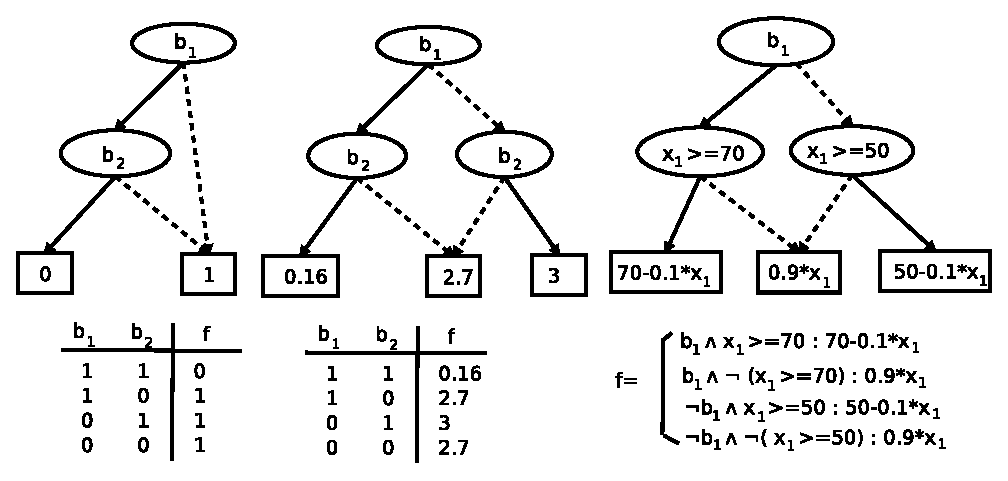
\includegraphics[width=0.7\textwidth]{FiguresSource/bddaddxadd.eps}
\vspace{-1mm}

\caption{%\footnotesize
Examples of decision diagrams: {\it (left)} a BDD, {\it (middle)} an ADD and {\it (right)} an XADD.}
\label{fig:bdd_add_xadd}
\end{figure}
%%%%%%%%%%%%%%%%%%%%%%%%%%%%%%%%%%%%%%%%%%%%%%%%%%%%%%%%%%%%%%%%%%%%%%%%%%

ADDs extend BDDs to allow real-valued ranges in the function representation ($\lbrace 0,1\rbrace^n \rightarrow \mathbb{R}$); they only differ from BDDs in the real-valued leaf nodes. There is a set of efficient operations for ADDs such as addition
($\oplus$), subtraction ($\ominus$), multiplication ($\otimes$),
division ($\oslash$), $\min(\cdot,\cdot)$ and $\max(\cdot,\cdot)$ (\cite{bahar93add}). Furthermore, BDDs and ADDs provide an efficient representation of \emph{context-specifically independent} defined as the following: 
\begin{mydef}
The set of variables $A$ and $B$ are \emph{context-specifically independent} given the set of variables $C$ and the context $c \in C$, denoted by $A \perp B | (C=c)$, if the following holds: 
\begin{align}
\mathit{P}(A | B,C=c) = \mathit{P}(A|C=c) \hspace{2mm} whenever \hspace{2mm} \mathit{P}(B,C=c) >0. \label{def:csi}
\end{align}
\end{mydef}

%As a simple example of the CSI property, consider the ADD representation of Figure~\ref{fig:bdd_add_xadd} (middle). This ADD represents the transition probability of $\mathit{P}(X'_1| X_2, a_{move})$ where the probability of $X'_1$ only depends on $X_2, a_{move}$. However in the context of $a_{move} = \mathit{false}$, $X'_1$ is also independent from $X_2$ since the probability is always zero in this case, i.e. $\mathit{P}(X'_1| X_2, a_{move}) = \mathit{P}(X'_1|  a_{move} = \mathit{false})$. 

%Parameterized ADD (PADD) is an extension of ADD that allows a compact representation of functions $\{0,1\}^{n} \rightarrow
%\mathbb{E}$, where $\mathbb{E}$ is the space of expressions
%parameterized by $\vec{p}$. For example, the ADD of Figure~\ref{fig:bdd_add_xadd} (middle) can be extended to a PADD to allow leaves such as $0.16p_1$ or $2.7+p_1$. PADDs are used as an efficient representation of factored MDPs with imprecise transitions \cite{spuddip}. 

XADDs extend ADDs to allow representing functions with both boolean and continuous variables, i.e. $\{0,1\}^{m} \times \mathbb{R}^n \rightarrow \mathbb{R}$. Here decisions can be boolean variable tests or continuous inequalities and leaves can be defined as arbitrary continuous expressions. We next formally define XADDs and the operations and algorithms required to solve HMDP problems using SDP. Pruning algorithms are then introduced to make this representation even more efficient. 

\subsection{XADD Formal Definitions}
\label{xaddformal}
An XADD is a function represented by a DAG involving variables $(\vec{b},\vec{x})$ where $b_i \in \{ 0,1 \}$ ($1 \leq i \leq m$) is a  boolean variable$\,$
and $x_j \in \left[ x_j^{min}, x_j^{max}\right]$ is a continuous variable, with $1 \leq j \leq n; x_j^{min}, x_j^{max} \in \mathbb{R}$ and  $x_j^{min}< x_j^{max}$.
An XADD structure consists of internal nodes (decision nodes) and leaf nodes (linear or nonlinear expressions).
XADD allows an efficient implementation of piecewise functions represented in general case partition notation (Definition \ref{defCase}).
{%\footnotesize 
Given a piecewise function:
\begin{align}
f = 
\begin{cases}
  \phi_1(\vec{b},\vec{x}): & f_1 (\vec{x})\\ 
 \vdots&\vdots\\ 
  \phi_k(\vec{b},\vec{x}): & f_k(\vec{x}), \\ 
\end{cases} \label{eq:function_xadd}
\end{align}
}
represented as an XADD $F$, each $f_i$ is a leaf node and each $\phi_i(\vec{b},\vec{x})$ (a logical formula) corresponds to a disjunction of the paths of decision nodes from root leading to the leaf $f_i$. For example, the XADD in Figure \ref{fig:inv_policy} (left) corresponds to the case statement of Equation \ref{eq:vfun_inv}.
Similar to ADDs, an XADD has a fixed ordering of decision tests from the root to a leaf where the low (l) or high (h) branch of each decision node determines the next node in the XADD. Similar to case statements that allow arbitrary functions,  a general XADD allows arbitrary decision nodes and leaf expressions. 
%However, in this paper, we restrict our functions to linear decisions and linear leaf expressions. This allows us to prune inconsistent linear constraints using an LP-solver, resulting, in general, in a more compact XADD. Next we provide the mathematical definition of \emph{linear XADDs}. %in the following: % Note that in the (or quadratic decisions that can be linearized). Also leaf expressions are assumed to be linear. 

\begin{mydef}(\textbf{Linear Expression}):
Giving a set of continuous variables $x_i$ and a set of constants $c_i$, a linear expression can be canonically defined  as the following:
\begin{equation}
\mathit{linearExpression} = c_0+\sum_{i} c_i x_i , 1 \leq i \leq n. 
\label{Eq:canonical}
\end{equation}
\end{mydef}

\begin{mydef}(\textbf{Linear XADD}):
Formally, an XADD with linear decisions and linear leaves expressions is defined using the following BNF grammar: 
\begin{equation}
\nonumber
\begin{array}{lll}
F&::=&  \mathit{linearExpression}  \hspace{1mm} \vert \hspace{1mm}   \mathit{decisionNode}\\
\mathit{decisionNode} &::=& \mathrm{if} (\mathit{F_{dec}})\ \mathrm{then}\ F \hspace{1mm} \mathrm{else}\ F \\ 
\mathit{F_{dec}} &::=& b \hspace{1mm}  \vert \hspace{1mm}  ( \mathit{linearExpression} \leq 0)  \hspace{1mm}\vert \hspace{1mm}
 ( \mathit{linearExpression} \geq 0)   
\\
%\mathit{linearExpression} &::=&c_0+\sum_{i} c_i x_i\\
b&::=& 0\hspace{1mm} |\hspace{1mm} 1
\end{array}
\end{equation}
\end{mydef}

A node $F$ of a Linear XADD is either a leaf node (also called terminal node) with a linear expression or a decision node (also called internal node) that contains a decision test $\mathit{F_{dec}}$ and two branches $F_h$ and $F_l$ (both of type F). When following an XADD path, if  $\mathit{F_{dec}}$ is true, branch $F_h$ is taken and if $\mathit{dec}$ is false, $F_l$ is taken. A decision node can be also represented by the triple $\langle F_{\mathit{dec}}, F_h, F_l \rangle$.
%%We will need this triple $\langle F_{\mathit{dec}}, F_h, F_l \rangle$ for the further sections.

The decision test $\mathit{F_{dec}}$ can be either a boolean variable $b\in \lbrace 0,1 \rbrace$ or a linear inequality over continuous variables $x_i$ \footnote {Note we assume continuous functions. Thus, in the boundary point (equality) of two expressions, they must have the same value. This continuous property allows us to replace $<$ ( $>$ ) with $\leq$ ( $\geq$ ).}. Figure~\ref{fig:bdd_add_xadd} (right) represents an XADD consisting of leaf nodes such as the node with the linear expression $0.9*x_1$ or decision nodes such as the nodes with the decision tests $b_1$ and $x_1 \geq 70$. 

We can also define a polynomial XADD involving polynomial Expressions defined next.

\begin{mydef}(\textbf{Polynomial Expression}):
Giving a set of continuous variables $x_i$ and a set of constants $c_i$, a polynomial  expression can be canonically defined  as the following:
\begin{equation}
\mathit{polynomialExpression} = \sum_{i} c_i \prod_{j} x_j^{P_{ij}}, 1 \leq i \leq k, 1 \leq j \leq n, 
\label{Eq:canonicalpoly}
\end{equation}
\end{mydef}

where k is the number of terms of the polynomial expression and $P_{ij}$ is the power of variable $x_j$ in the i-th term. 

\begin{mydef}(\textbf{Polynomial XADD}):
Formally, an XADD with polynomial decisions and polynomial leaves expressions is defined using the following BNF grammar: 
\begin{equation}
\nonumber
\begin{array}{lll}
F&::=&  \mathit{polynomialExpression}  \hspace{1mm} \vert \hspace{1mm}   \mathit{decisionNode}\\
\mathit{decisionNode} &::=& \mathrm{if} (\mathit{F_{dec}})\ \mathrm{then}\ F \hspace{1mm} \mathrm{else}\ F \\ 
\mathit{F_{dec}} &::=& b \hspace{1mm}  \vert \hspace{1mm}  ( \mathit{polynomialExpression} \leq 0)  \hspace{1mm}\vert \hspace{1mm}
 ( \mathit{polynomialExpression} \geq 0)   
\\
%\mathit{linearExpression} &::=&c_0+\sum_{i} c_i x_i\\
b&::=& 0\hspace{1mm} |\hspace{1mm} 1
\end{array}
\end{equation}
\end{mydef}

Note that a special case of polynomial XADD are the univariate quadratic XADDs, where the expressions are 
in the form of $c_0+ c_1 x_j^2 + \sum_{i} c_i x_i$  $(2 \leq i \leq n)$. Since the univariate quadratic can be linearized, it can be transformed into a Linear XADD.

As we can evaluate a piecewise function with a given variable assignment, an XADD (linear or polynomial) can be evaluated as we define next.

\begin{mydef}(\textbf{XADD Evaluation}):
Given (linear or polynomial) XADD F  that represents functions of type $\lbrace 0,1 \rbrace^m \times \mathbb{R}^{n} \rightarrow \mathbb{R}$ and a variable assignment $\vec{\rho} \in \lbrace \lbrace0,1 \rbrace^m,\mathbb{R}^n \rbrace$ to $(\vec{b},\vec{x})$, an XADD evaluation,  
$ Val(F,\vec{\rho})$, is a real value.  $ Val(F,\vec{\rho})$ can be computed recursively by:
\begin{equation*}
Val(F,\vec{\rho}) = \left\{
\begin{array}{lll}
\vec{\rho}(\mathit{F}),  &\textrm{if } F=\mathit{Expression}\\
\mathit{Val} (F_h,\vec{\rho}), &\textrm{if } F = \mathit{decisionNode} \langle F_{\mathit{dec}}, F_h, F_l \rangle \hspace{2mm}  \mathit{and} \hspace{2mm} \vec{\rho}(\mathit{F_{dec}})=\mathit{true}\\
 \mathit{Val} (F_l,\vec{\rho}), &\textrm{if } F = \mathit{decisionNode} \langle F_{\mathit{dec}}, F_h, F_l \rangle \hspace{2mm}  \mathit{and}  \hspace{2mm} \vec{\rho}(\mathit{F_{dec}})=\mathit{false},\\
\end{array} \right. 
\end{equation*}
where $\vec{\rho}(\mathit{F}) \in \mathbb{R}$, for $ F=\mathit{Expression}$ is the value of $F$ in the variable assignment $\vec{\rho}$. $\vec{\rho}(\mathit{F_{dec}})$  (a relational expression) is the value of $\mathit{F_{dec}}$  in the variable assignment $\vec{\rho}$, that can be true or false.


This recursive definition reflects the structural
evaluation of $F$ starting at its root node and following
the corresponding branch at each decision node according to $\vec{\rho}(F_\mathit{dec})$.
The evaluation continues until a leaf node F has been reached,
which then returns $\vec{\rho}(\mathit{F})$. As an example, in Figure~\ref{fig:bdd_add_xadd} (right), an assignment of $\vec{\rho} = \lbrace 1, 90\rbrace$ to $(b_1,x_1)$ yields to $Val(F,\vec{\rho})=8.1$.
\end{mydef}

%%%%%%%%%%%%%%%%%%%%%%%%%%%%%%%%%%%%%%%%%%%%%%%%%%%%%%%%%%
\begin{mydef}(\textbf{Path Formula}):
Let $C=(F^0,F^1,F^2 , \cdots, F^{\mathit{k}})$ be a path of nodes of an XADD $F$, from root to $F^k$ (where $F^k$ can be either a leaf node or a decision node). A path formula $\psi(C)$ is definided as:
\begin{equation}
\psi(C) \equiv \bigwedge_{i=0}^{\mathit{k}-1}
\begin{cases}
 \mathit{F^i_{dec}} & if \hspace{2mm}  F^{i+1}= F^i_h\\ 
 \neg \mathit{F^i_{dec}} & if \hspace{2mm} F^{i+1}=F^i_l. \\ 
\end{cases} \label{eq:path}%), (F_2,\rho(F_2)), \cdots, (F_i,\rho(F_i)) \rangle
\end{equation}
\end{mydef}

Figure~\ref{fig:path} shows an XADD with formulas associated to each path ending at a decision node or leaf node. For instance, the path $C=(n_1, n_2, n_3)$ defines a path formula $\psi(C)=\neg (x \geq -8) \wedge \neg (x \leq -12)$.

\begin{figure}[t!]
\centering
%\subfigure{
%\hspace{-20mm}
%\vspace{-3mm}
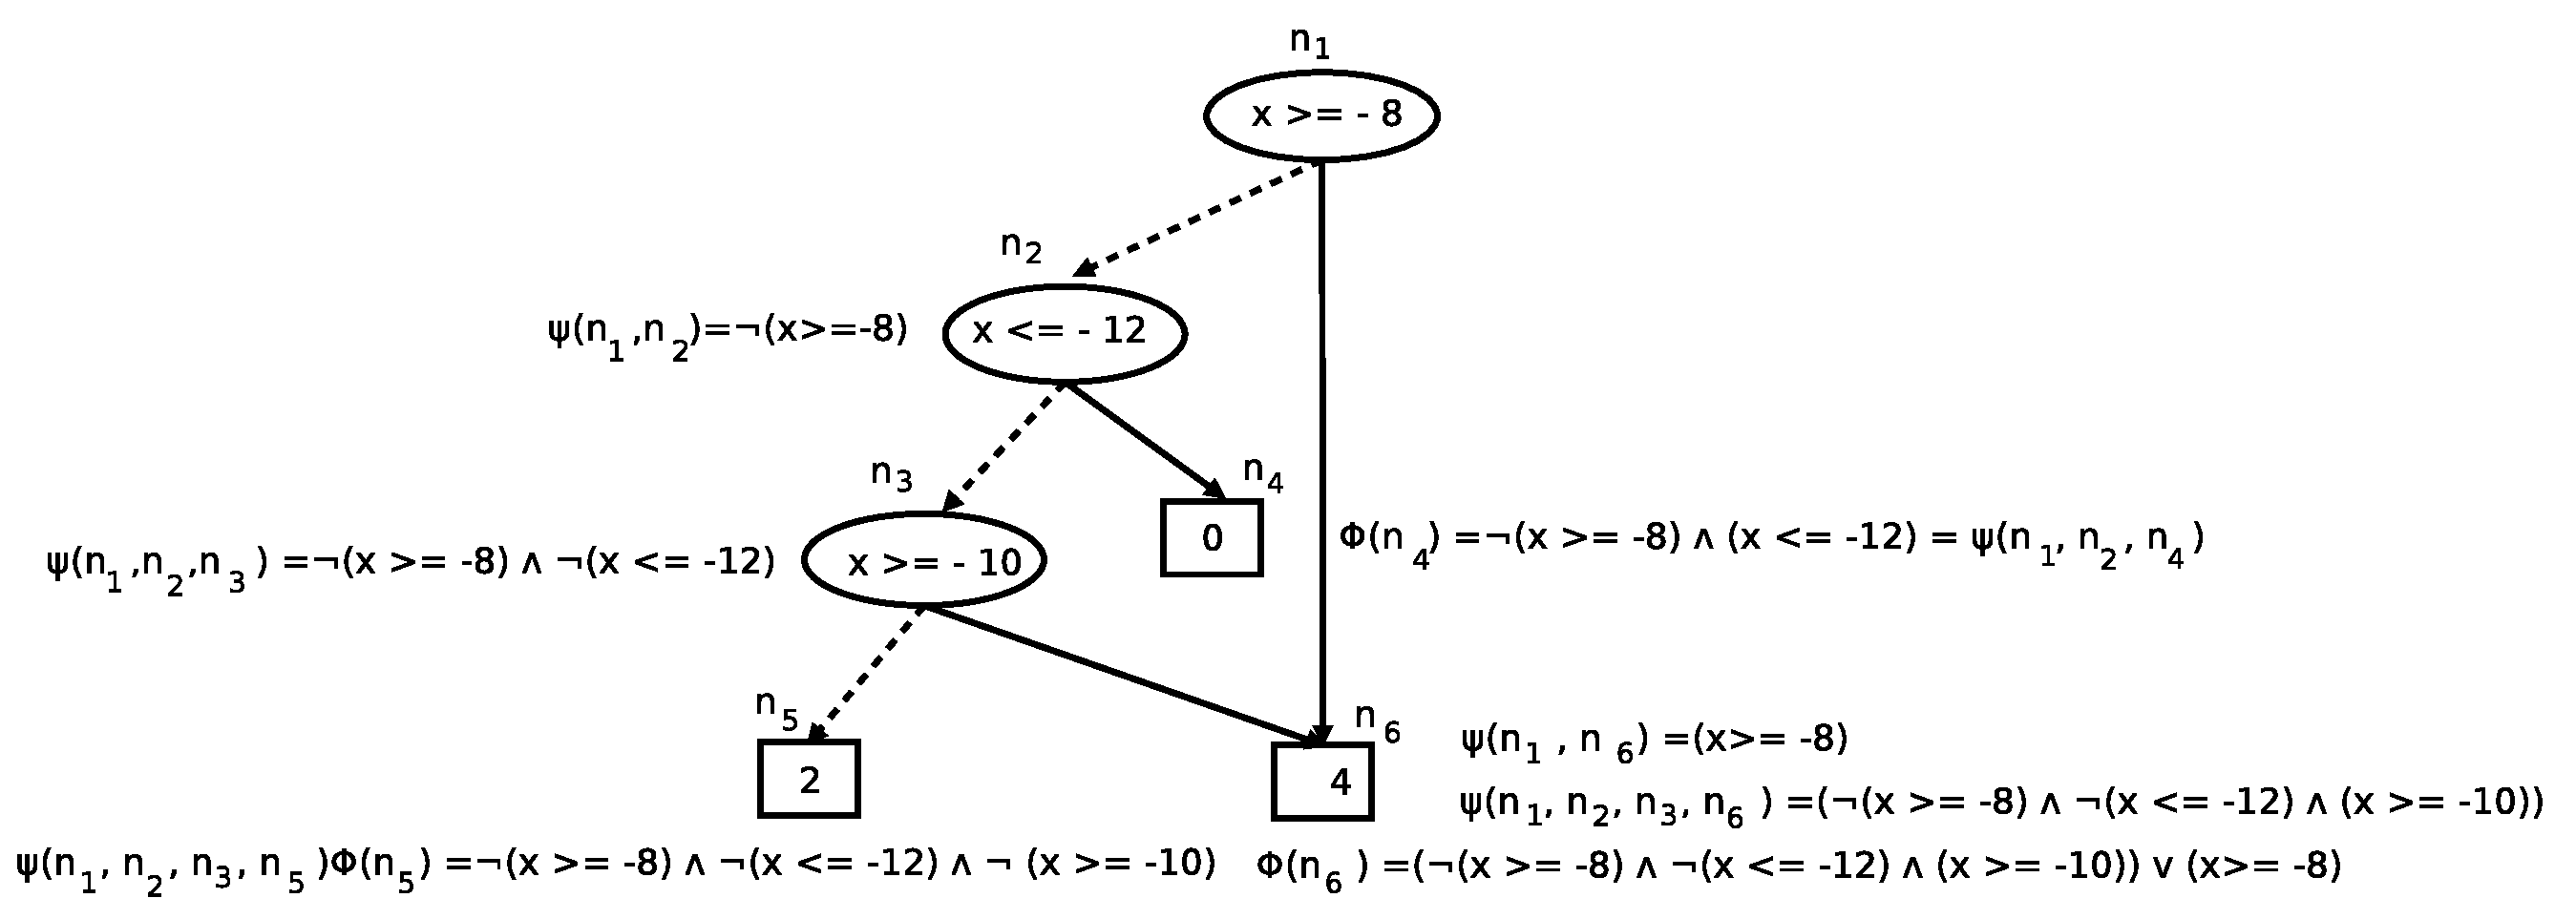
\includegraphics[width=1\textwidth]{FiguresSource/path.eps}
%\vspace{-3mm}
%\hspace{1mm}
%\includegraphics[width=0.18\textwidth]{xaddFig/counterexample.pdf}
\vspace{-2mm}
\caption{%\footnotesize 
Path formulas and case partitions in an XADD.}
\label{fig:path}
%\vspace{-4mm}
\end{figure}
%%%%%%%%%%%%%%%%%%%%%%%%%%%%%%%%%%%%%%%%%%%%%%%
Recall the leaf node $F^i$ has the value $f_i$ in the case representation of Equation~\ref{eq:function_xadd}. We can now formally define a \emph{case partition} 
$\langle \phi_i(\vec{b},\vec{x}): f_i(\vec{x})\rangle$ using the path formula definition. 

\begin{mydef}(\textbf{Case Partition}): Let $F^i$ be a leaf node of an XADD; and $\mathbb{C}= \{C_1^i, \cdots, C_d^i\} $ be all paths from the root to $F^i$. A case partition $\phi(F^i)$ is the disjunction of the path formula for each path in $\mathbb{C}$, i.e.: 

\begin{equation}
\phi(F^i) \equiv \bigvee_{j=1}^{d} \psi(C_j^i), \label{eq:casePartition}
\end{equation} 
\end{mydef}
i.e., a disjunction of all paths that leads to the node $F^i$.
For example,  in Figure \ref{fig:path}, a case partition for the leaf node with value equal to 4 $(n_6)$ is $\phi (n_6)=\{(x \geq -8) \vee (\neg (x \geq -8) \wedge \neg(x \leq -12) \wedge ( x\geq -10))\}$.

\begin{mydef}(\textbf{XADDs equivalency}): Let $f^1$ and $f^2$ be two piecewise functions represented by the XADDs $F^1$ and $F^2$, respectively. $F^1$ is equivalent to $F^2$ (denoted by $F^1 \equiv F^2$) if $f^1(\vec{b}, \vec{x}) = f^2(\vec{b}, \vec{x}), \forall (\vec{b}, \vec{x})$.
\end{mydef}

Another important aspect of an XADD is the introduction of redundant nodes or nodes that result in inconsistent path formula.

\begin{mydef}(\textbf{Inconsistent path formula}):
A path formula $\psi$ in XADD $F$ is inconsistent if $\psi \models \perp$.
\end{mydef}
The XADD of Figure~\ref{fig:inconsistent_XADD} has an inconsistent path formula for path $C=(n_1, n_2, n_4)$ on which the decision $\neg(x \geq -10)$ violates the previous constraint of $x\geq -8$ (in $n_1$), i.e.: $(x \geq -8) \wedge \neg(x \geq -10) \models\perp$.  

\begin{mydef}(\textbf{Redundant node}):
A redundant node occurs in an XADD where two nodes give the same function definition and removing one does not change any of the partitions of that function. A decision node $F$ is redundant if it can be replaced by one of its branches. That is, $F \equiv F_h$ or $F \equiv F_l$ (according with XADD equivalency definition). 
\end{mydef}

As an example, consider the XADD of Figure~\ref{fig:redundant_XADD} where removing node $n_1$ will not affect the XADD function: if $x < - 8$ then $f^{n_1}(x)=f^{n_2}(x)$, otherwise ($x >= - 8$) $f^{n_1}(x)=f^{n_2}(x)=4$. Therefore $F^{n_1} \equiv F^{n_1}_l$ and thus $n_1$ is redundant.  

In the next  section we will present algorithms that can detect and prune inconsistent paths and redundant nodes of an XADD. 


%%%%%%%%%%%%%%%%%%%%%%%%%%%%%%%%%%%%%%%%%%%%%%%%%%%%%%%%%%%%%%%%%%%%%%%%%%
\begin{figure}[t!]
\centering
%\subfigure{
%\hspace{-20mm}
%\vspace{-3mm}
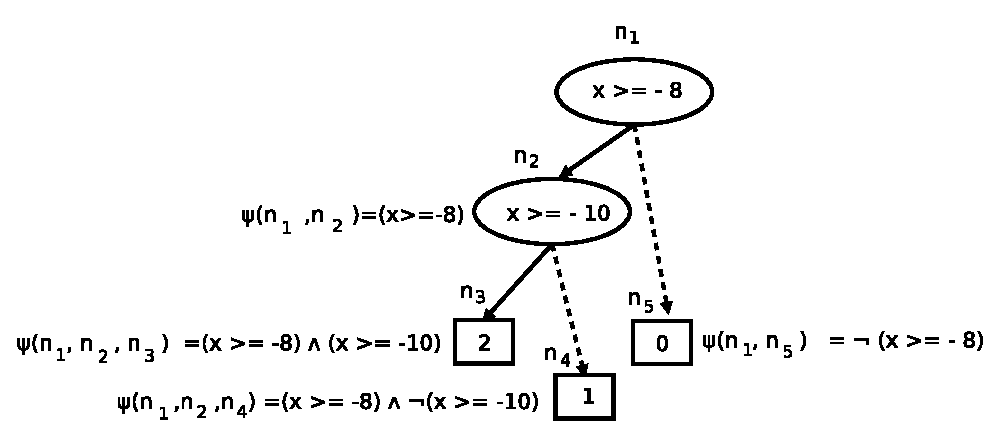
\includegraphics[width=0.8\textwidth]{FiguresSource/consistency.eps}
% * <karinaval@gmail.com> 2016-04-18T13:42:42.245Z:
%
% > Prunning
%
% ^.
%\vspace{-3mm}
%\hspace{1mm}
%\includegraphics[width=0.18\textwidth]{xaddFig/counterexample.pdf}
\vspace{-2mm}
\caption{%\footnotesize 
XADD with an Inconsistent Path Formula $\psi(n_1, n_2, n_4)$, i.e. $((x \geq -8) \wedge \neg (x \geq -10) \models\perp)$. 
}
\label{fig:inconsistent_XADD}
%\vspace{-4mm}
\end{figure}


\begin{figure}[t!]
\centering
%\subfigure{
%\hspace{-20mm}
%\vspace{-3mm}
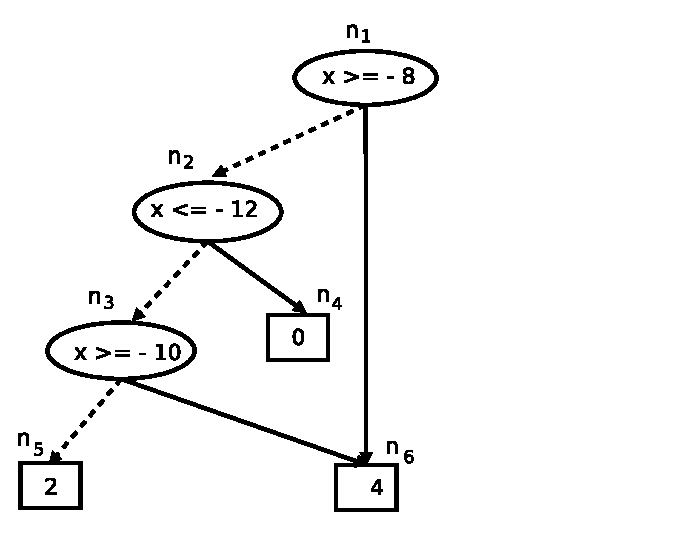
\includegraphics[width=0.5\textwidth]{FiguresSource/redundancy.eps}
%\vspace{-3mm}
%\hspace{1mm}
%\includegraphics[width=0.18\textwidth]{xaddFig/counterexample.pdf}
\vspace{-2mm}
\caption{%\footnotesize 
XADD with a Redundant Node $n_1$: it is redundant since $n_2$ represents the same function as $n_1$, i.e., $F^{n_1} \equiv F^{n_1}_l$.}
\label{fig:redundant_XADD}
%\vspace{-4mm}
\end{figure}
%%%%%%%%%%%%%%%%%%%%%%%%%%%%%%%%%%%%%%%%%%%%%%%%%%%%%%%%%%




%%%%%%%%%%%%%%%%%%%%%%%%%%%%%%%%%%%%%%%%%%%%%%%%%%%%%%%%%%%%%%%%%%%%%%%%%%
\subsection{XADD Operations}
\label{sec:xaddoperations}

One of the most important feature of XADDs is to compactly represent a piecewise function $f$. There are two main functions used to make a more compact (reduced) representation of an XADD: Reduce and GetNode. A reduced XADD is an XADD where identical branches are merged. The function Reduce calls GetNode to create a new XADD node or merge identical branches of a node. 


\subsubsection{Reduce and GetNode}

The function \emph{GetNode} returns a compact representation of a single internal decision node of an XADD (Algorithm \ref{algGetNode}). \emph{GetNode} is called by several XADD algorithms we will introduce. It checks the branches of a node $F$ so that it does not have identical $F_h$ and $F_l$. If a repeated branch is found, it simply returns one of them (Lines 4--5 of Algorithm \ref{algGetNode}). Otherwise this function must build a new node with a unique id. Each new id is stored in a  \emph{NodeCache} hash table. Before adding a new node, the cache is checked for an identical node (Lines 7--9 of Algorithm \ref{algGetNode}). 

%%%%%%%%%%%%%%%%%%%%%%%%%%%%%%%%%%%%%%%%%%%%%%%%%%%%%%%%%%%%%%%%%
\incmargin{.5em}
\begin{algorithm}[t!]
\SetKwInOut{Input}{input}
\SetKwInOut{Output}{output}
\dontprintsemicolon
\Begin{
   //NodeCache is a hash table that stores an id to each node $F$\\
   //redundant branches\\
   \If{$F_l = F_h$} 
   {
      \Return{$F_l$}\;
   }
   id $\leftarrow$ NodeCache($\langle F_{\mathit{dec}}, F_h, F_l \rangle)$ \\ 
  //check if the node already exists\\
   \If{$\mathit{id}=$null}
   {id\ $\leftarrow$ new unallocated id\;  
    NodeCache($\langle F_{\mathit{dec}}, F_h, F_l \rangle) \leftarrow \mathit{id}$ \;
   }
   \Return{id}\;
}
\caption{{\sc GetNode}($F_{\mathit{dec}}, F_h, F_l$) $\longrightarrow \langle F^r \rangle$\label{algGetNode}}
\end{algorithm}
\decmargin{.5em}
%%%%%%%%%%%%%%%%%%%%%%%%%%%%%%%%%%%%%%%%%%%%%%%%%%%%%%%%%%%%%%%%

The function \emph{ReduceXADD} (Algorithm \ref{algReduceXADD}) allows the construction of a compact XADD representation for a given decision diagram. This algorithm recursively constructs a reduced XADD from the bottom up. 
If $F$ is a leaf node, i.e. a linear expression, the algorithm returns the canonical form of $F$ (Equation \ref{Eq:canonical}) (Lines 5--6 of Algorithm \ref{algReduceXADD}).  If $F$ is a decision node then the algorithm recursively computes the reduced XADDs of the low and high branches and returns a final reduced XADD $F^r$ (Lines 8--14 of Algorithm \ref{algReduceXADD}).
Note that for a decision node $\langle F_{\mathit{dec}}, F_h, F_l \rangle$, $F_h$ and $F_l$ are the id for high and low branches, respectively. 
Algorithm \ref{algReduceXADD} uses the \emph{GetNode} function in Line 12 to merge identical branches. 
%Paths are checked for inconsistency in line 12 which performs the forthcoming Algorithm~\ref{algPrune} and the $\mathit{true}$ parameter also allows checking for redundant nodes. 
The reduced XADD $F^r$ is then stored in the \emph{ReduceCache} hash table. \emph{ReduceCache} ensures that each node is visited only once by Algorithm \ref{algReduceXADD}; it has linear running time according to the number of nodes in $F^r$.
%%%%%%%%%%%%%%%%%%%%%%%%%%%%%%%%%%%%%%%%%%%%%%%%%%%%%%%%%%%%%%%%%
\incmargin{.5em}
\linesnumbered
\begin{algorithm}[t!]
\SetKwFunction{getNode}{{\sc GetNode}}
\SetKwFunction{reduce}{{\sc ReduceXADD}}
\SetKwFunction{redundant}{{\sc PruneRedundancy}}
\SetKwInOut{Input}{input}
\SetKwInOut{Output}{output}
\dontprintsemicolon
%\Input{$F$ (root node id for an arbitrary ordered decision diagram)}
%\Output{$F_r$ (root node id for reduced XADD)}
%\BlankLine
\Begin{
   //F is a root node id for an arbitrary ordered decision diagram\\
   //$F^r$ is a root node id for the reduced XADD\\
  // ReduceCache is a hash table that stores previously redundant XADDs\\
   \If{F is terminal node}
   {
   \Return{terminal node for $F$, i.e., a canonical linear expression}\;
   }
   //else reduce decision node $F$\\
   $F^r \leftarrow$ ReduceCache($F)$\\  
   \If{$F^r$ = null}
   {
    $F_h \leftarrow$ \reduce{$F_h$}\;
    $F_l \leftarrow$ \reduce{$F_l$}\;
    //get a canonical internal node id\\
    $F^r \leftarrow$ \getNode{$F_{\mathit{dec}}$, $F_h$, $F_l$}\;
    %$F_r = $ \redundant{$F$, $\psi$,$\mathit{true}$}\;
    ReduceCache ($F) \leftarrow F^r$ \;
   } 
   \Return{$F^r$}\;
}
\caption{{\sc ReduceXADD}($F$) $\longrightarrow$ $\langle F^r \rangle$ \label{algReduceXADD}}
\end{algorithm}
\decmargin{.5em}
%%%%%%%%%%%%%%%%%%%%%%%%%%%%%%%%%%%%%%%%%%%%%%%%%%%%%%%%%%%%%%%%%
As in the case representation, the symbolic operations required to perform SDP (Section \ref{sec:caserep})  can be also performed using XADD operations, mainly categorized into unary and binary operations.   


\subsubsection{Unary XADD Operations}

According to Section \ref{SDP} the unary operations required in SDP are scalar multiplication ($c.f$), negation ($- f$), restriction ($f|_\phi$), marginalization ($\sum_{b_i}f$), substitution ($f_\sigma$), integration  ($\int_x f$) and continuous maximization ($\max_{\vec{y}} f$) and linearize, where $f$ is a piecewise linear function, $c \in \mathbb{R}$, $\phi$ is a logical formula and $\sigma$ is a set of variables and their substitution. In this section we briefly describe how this operations are performed using XADD representation.

\emph{Scalar multiplication}, $c.F$, where $c \in \mathbb{R}$ and F is an XADD is performed by multiplying all the XADD leaves by $c$ while \emph{negation} of an XADD $F$ is the multiplication  $-1.F$.

The \emph{restriction} operation for an XADD ($F|_{\phi}$) is done only over binary variables. Thus $\phi$ is of the form $b_i=true$ or  $b_i=false$. Restriction of an XADD $F$ to some formula $\phi$ is performed by making a conjunction of $\phi$ to each case partition  $\phi_i$, i.e., $\phi_i \wedge \phi $. This is equal to taking the true or false branch of the decision node $b_i$.
This operation can also be used for \emph{marginalizing boolean variables}, represented by $\sum_{b_i}$ which eliminates variable $b_i$ from $F$  by computing the sum  $F|_{b_i=true} \oplus \ F|_{b_i=false}$ (the $\oplus$ binary operation is performed by Algorithm~\ref{algApply} described in the next section). Figure~\ref{fig:restrict} illustrates the operations  $F|_{d=true}$, $F|_{d=false}$ and  $\sum_{d}F$. 

%%%%%%%%%%%%%%%%%%%%%%%%%%%%%%%%%%%%%%%%%%%%%%%%%%%%%%%%%%%%%%%%%%%%%%%%%%%%
%\vspace{10mm}
\begin{figure}[t!]
\centering
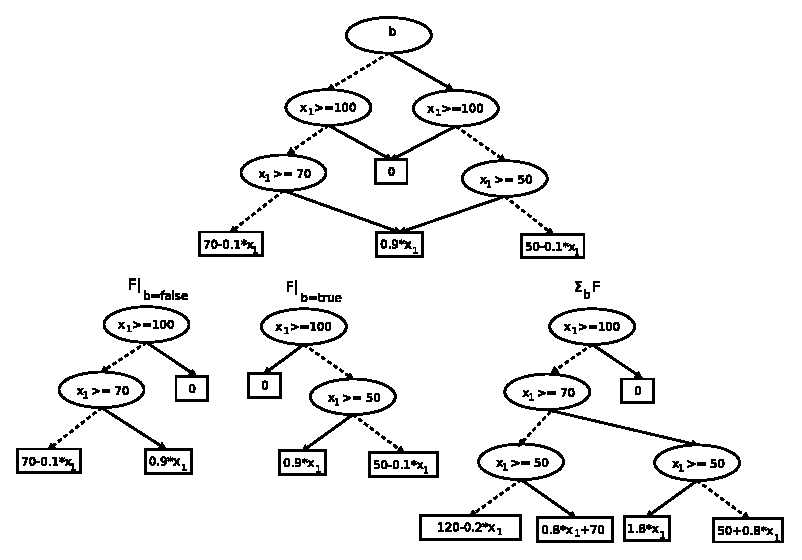
\includegraphics[width=1\textwidth]{FiguresSource/restriction.eps}
%\vspace{-2mm}

\caption{%\footnotesize 
{\it (bottom left)} Example of restriction operation $F|_{b=true}$ and $F|_{b=false}$ on the XADD F (top). {\it (bottom right)} The resulting XADD after marginalization $\sum_{b}F$.}
\label{fig:restrict}
%\vspace{-6mm}
\end{figure}
%%%%%%%%%%%%%%%%%%%%%%%%%%%%%%%%%%%%%%%%%%%%%%%%%%%%%%%%%%%%%%%

 
\emph{Substitution} of a given XADD $F$ by $\sigma$ is performed by applying $\sigma$ in each case statement as in Equation \ref{SubEq}. The substitution operand affects both leaves and decision nodes and changes them according to the variable substitution. 
Decisions may become unordered after the substitution operation  and a reorder algorithm has to be applied after this operation. Algorithm~\ref{alg:reorder} reorders an XADD $F$ by recursively applying  operations of $\otimes$ and $\oplus$ to decision nodes. Note that $\mathbb{I}[\mathit{F_{dec}}]$ is the indicator function for $F_{dec}$, i.e.:

{%\footnotesize 
\begin{align*}
\mathbb{I}[\mathit{F_{dec}}] = 
\begin{cases}
  F_{dec}: & 1 \\ 
  \neg F_{dec}: & 0 \\ 
\end{cases}
\end{align*}
}

Similarly to previous algorithms, a \emph{ReorderCache} is used to prevent unnecessary computations. An example of the application of reorder is shown in Figure \ref{fig:reorder}, which reorder the XADD of Figure \ref{fig:bdd_add_xadd}(right), with the new order of nodes given by: Order($x_1>=70$) $<$ Order($x_1>=50$) $<$ Order($b_1$). The computation of $F_h$ and $F_l$ (lines 7 and 8 of Algorithm \ref{alg:reorder}) are showed in Figure \ref{fig:reorder}(a) and Figure \ref{fig:reorder}(b), respectively. Finally, the resulting XADD $F^r$ is shown in Figure \ref{fig:reorder}(c). 

\begin{figure}[t!]
\centering
%\subfigure{
%\hspace{-20mm}
%\vspace{-3mm}
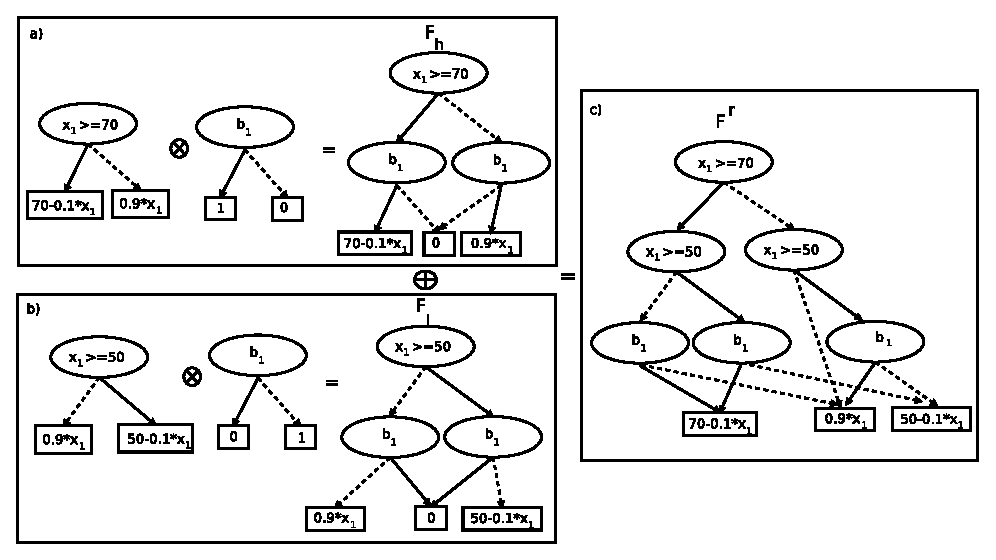
\includegraphics[width=1\textwidth]{FiguresSource/reorder.eps}
%\vspace{-3mm}
%\hspace{1mm}
%\includegraphics[width=0.18\textwidth]{xaddFig/counterexample.pdf}
\vspace{-2mm}
\caption{%\footnotesize 
Applying reorder on the XADD of Figure \ref{fig:bdd_add_xadd} (right) with the new order of nodes given by: Order($x_1>=70$) $<$ Order($x_1>=50$) $<$ Order($b_1$). (a) The resulting reorder XADD $F_h$. (b) The resulting reorder XADD $F_l$. (c) The resulting reordered XADD $F^r$.} 
\label{fig:reorder}
%\vspace{-4mm}
\end{figure}


%%%%%%%%%%%%%%%%%%%%%%%%%%%%%%%%%%%%%%%%%%%%%%%%%%%%%%%%%%%%%%%%%
\incmargin{0.5em}
\linesnumbered
\begin{algorithm}[t!]
\SetKwFunction{getCanonicalNode}{{\sc GetCanonicalNode}}
\SetKwFunction{reduce}{{\sc Reorder}}
\SetKwInOut{Input}{input}
\SetKwInOut{Output}{output}
\dontprintsemicolon

%\Input{$F$ (root node for possibly unordered XADD)}
%\Output{$F_r$ (root node for an ordered XADD)}
\BlankLine
\Begin{
   \If{F is a terminal node}
   {
   \Return{canonical terminal node of $F$}\;
   }
    // If F is not a terminal node, F is $\langle  F_{\mathit{dec}}$, $F_h$, $F_l \rangle$\\
    $F^r \leftarrow$  ReorderCache(F)\\ 
   \If{$F^r = $null}
   {
    $F_{\mathit{h}} \leftarrow$ \reduce{$F_{\mathit{h}}$} $\otimes \; \mathbb{I}[\mathit{F_{dec}}]$ \;
    $F_{\mathit{l}} \leftarrow$ \reduce{$F_{\mathit{l}}$} $\otimes \; \mathbb{I}[\neg \mathit{F_{dec}}]$\;
    $F^r \leftarrow F_{\mathit{h}} \oplus F_{\mathit{l}}$\;
    ReorderCache$(F) \leftarrow F^r$ \;
   } 
   \Return{$F^r$}\;
}
\caption{{\sc Reorder}($F$) $\longrightarrow$ $\langle F^r \rangle$ \label{alg:reorder}}
\end{algorithm}
\decmargin{0.5em}
%%%%%%%%%%%%%%%%%%%%%%%%%%%%%%%%%%%%%%%%%%%%%%%%%%%%%%%%%%%%%%%%%

As we have seen in Section \ref{MargContVar}, \emph{marginalizing a continuous variable} $y$ is performed using the integration of the $\delta$-function on variable $y$. In particular for SDP we require computing $\int_{y} \delta [ y - g(\vec{x})]fdy$ which triggers the substitution $f \lbrace y/ g(\vec{x})\rbrace$ on $f$.
% Note that the XADD representation is used for both functions $f$ and $g$.


The unary operation \emph{linearize} takes an XADD F with linear and univariate quadratic decision nodes and transforms into an XADD $F^r$ where all decision nodes are linear decisions.
The Linearize algorithm (Algorithm~\ref{algLinearize}) similarly to other XADD algorithms uses a \emph{LinearCache} to avoid linearizing the same node. For each node in the XADD starting at the root node, the algorithm linearizes the decision node using \emph{LinearizeDecisionNode} that finds the roots of the non-linear function and creates new linear decisions with these roots. By recursively applying this algorithm on the low and high branches, all nodes of $F$ are linearized.

%%%%%%%%%%%%%%%%%%%%%%%%%%%%%%%%%%%%%%%%%%%%%%%%%%%%%%%%%%%%%%%%%
\incmargin{0.5em}
\linesnumbered
\begin{algorithm}[t!]
\dontprintsemicolon
\SetKwFunction{getRoots}{{\sc LinearizeDecisionNode}}
\SetKwFunction{reduce}{{\sc Linearize}}
\SetKwInOut{Input}{input}
\SetKwInOut{Output}{output}

%\Input{$F$ (root node id for an arbitrary ordered decision diagram)}
%\Output{$F_r$ (root node id for linearized XADD)}
\BlankLine
\Begin{
   \If{F is terminal node}
   {
   \Return{canonical terminal node of $F$}\;
   }
   $F^r \leftarrow$ LinearCache($F)$ \\
    \If{$F^r =$ null}
   {
   //use recursion to reduce sub diagrams\\
    $F_h \leftarrow$  \reduce{$F_h$}\;
    $F_l \leftarrow$ \reduce{$F_l$}\;
    //get a linearized internal node id\\
    $F^r \leftarrow$ \getRoots{$\mathit{F_{dec}}$, $F_h$, $F_l$}\;
    LinearCache($F) \leftarrow F^r$ \;
   } 
   \Return{$F^r$}\;
}
\caption{{\sc ReduceLinearize}($F$)$\longrightarrow$ $\langle F^r \rangle$  \label{algLinearize}}
\end{algorithm}
\decmargin{.5em}
%%%%%%%%%%%%%%%%%%%%%%%%%%%%%%%%%%%%%%%%%%%%%%%%%%%%%%%%%%%%%%%%%	

Finally, the other operation required to solve CA-HMDPs using SDP is the \emph{continuous maximization} ($\max_{\vec{y}} f$) over continuous action parameters $\vec{y}$. As we have seen in Section \ref{contmax}, it suffices to provide just the univariate $\max_{y}$ solution, to be performed at each case partition and the max of each partition can be computed by Equation \ref{eq:casemax_max}. The operation of continuous maximization can also be defined using XADDs. As we have defined in Section \ref{xaddformal} each XADD path from root to leaf node is treated as a single case partition with conjunctive constraints. 

An example of $\max_{\vec{y}} f$ for a single case partition is presented in Figures ~\ref{fig:step123:xadd_max}, \ref{fig:step4:xadd_max}, \ref{fig:step5:xadd_max} and \ref{fig:step6:xadd_max} using XADD representation. This example is more complex compared to the CAIC partition mentioned in Section \ref{section:SVI} since it involves a case partition with a quadratic expression leaf. The six steps  follows the procedure specified in Section \ref{contmax} for the maximum of a single case partition: (1) finding the sets UB,LB, Root, and Ind; (2) compute HLB and LUB; (3) apply the substitution operator $\{y/f\}$, with Root, HLB and LUB; (4) Compute the conditions $HLB \leq LUB$ and $HLB \leq \Root \leq LUB$ (5) compute $\casemax$ of the substitutions result; and (6) computing the final result as a new case partition Equation \ref{eq:maxcasepartition}.

% TODO: Dont we need to specify an algorithm to continuous maximixation and SDP 
% using XADDs? 

%\begin{landscape}
 \begin{figure}
 \centering
 \begin{minipage}{0.25\linewidth}
 \centering
  \scalebox{0.8}{
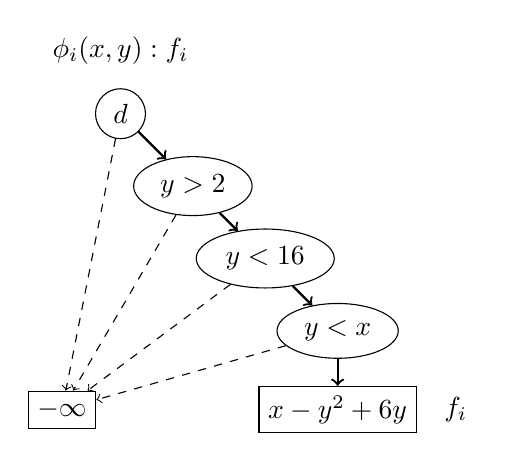
\begin{tikzpicture}[auto]
	% title node
	\node [novertex] (N0) {$\phi_i(x,y) : f_i$};

	% place nodes
	\node [root, below of=N0, node distance=0.8cm]        (N1) {$d$};
	\node [inode, below right of=N1, node distance=1.3cm] (N2) {$y > 2$};
	\node [inode, below right of=N2, node distance=1.3cm] (N3) {$y < 16$};
	\node [inode, below right of=N3, node distance=1.3cm] (N4) {$y < x$};
	\node [terminal, below of=N4, node distance=1.0cm]    (N5) {$x - y^2+6y$};
	\node [terminal, left of=N5, node distance=3.5cm]     (N6) {$-\infty$};
    
	\node [novertex, right of=N5, node distance=1.5cm]    (N7) {$f_i$};

	% draw edges
    \path [high] (N1) -- (N2);
    \path [high] (N2) -- (N3);
    \path [high] (N3) -- (N4);
    \path [high] (N4) -- (N5);
    
    \path [low] (N1) -- (N6);
    \path [low] (N2) -- (N6);
    \path [low] (N3) -- (N6);
    \path [low] (N4) -- (N6);
\end{tikzpicture}
}

  \end{minipage}
 \begin{minipage}{0.7cm}
 $\Longrightarrow$
  \end{minipage}
  \begin{minipage}{0.09\linewidth}
 \centering
 \scalebox{0.8}{
\framebox[1.0\width]{
\minibox{
$\textnormal{UB} = \{x,16\}$ \\

$\textnormal{LB} = \{2\}$ \\

$\textnormal{Ind} = \{d\}$ \\

$\textnormal{Root} = 3$\\
}
}
}
 \end{minipage}
 \begin{minipage}{0.8cm}
 \centering
 %\rotatebox{45}{$\rightarrow$}

 \hspace{14mm}
 %\rotatebox{-45}{$\rightarrow$}
 \end{minipage}
 \begin{minipage}{0.12\linewidth}
 \centering

 \vspace{-15mm}

 \scalebox{0.8}{
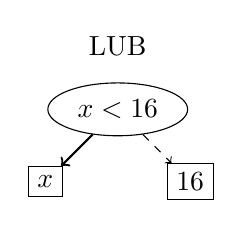
\begin{tikzpicture}[auto]
	% title node
	\node [novertex] (N0) {LUB};

	% place nodes
	\node [inode, below of=N0, node distance=0.8cm]          (N1) {$x < 16$};
	\node [terminal, below left of=N1, node distance=1.3cm]  (N2) {$x$};
	\node [terminal, below right of=N1, node distance=1.3cm] (N3) {$16$};

	% draw edges
    \path [high] (N1) -- (N2);
    \path [low] (N1) -- (N3);
\end{tikzpicture}
}

 \vspace{15mm}

 \scalebox{0.8}{
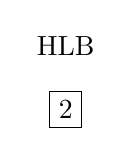
\begin{tikzpicture}[auto]
	% title node
	\node [novertex] (N0) {HLB};

	% place nodes
	\node [terminal, below of=N0, node distance=0.8cm] (N1) {$2$};

	% draw edges

\end{tikzpicture}
}
 \vspace{15mm}

 \scalebox{0.8}{
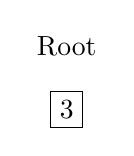
\begin{tikzpicture}[auto]
	% title node
	\node [novertex] (N0) {Root};

	% place nodes
	\node [terminal, below of=N0, node distance=0.8cm] (N1) {$3$};

	% draw edges

\end{tikzpicture}
}
  \end{minipage}
\begin{minipage}{1.cm}
 \centering
 \small
\vspace{-10mm}
 \emph{subst}\\
 $\Longrightarrow$

 \vspace{25mm}

 \emph{subst}\\
 $\Longrightarrow$
 \vspace{20mm}

 \emph{subst}\\
 $\Longrightarrow$

\end{minipage}
 \begin{minipage}{0.20\linewidth}
 \centering
 \vspace{-15mm}

 \scalebox{0.8}{
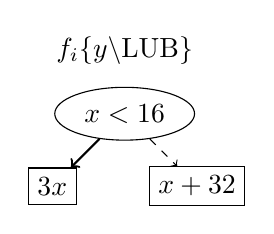
\begin{tikzpicture}[auto]
	% title node
	\node [novertex] (N0) {$f_i\{y \backslash \textnormal{LUB}\}$};

	% place nodes
	\node [inode, below of=N0, node distance=0.8cm]          (N1) {$x < 16$};
	\node [terminal, below left of=N1, node distance=1.3cm]  (N2) {$3x$};
	\node [terminal, below right of=N1, node distance=1.3cm] (N3) {$x+32$};

	% draw edges
    \path [high] (N1) -- (N2);
    \path [low] (N1) -- (N3);
\end{tikzpicture}
}

 \vspace{15mm}

 \scalebox{0.8}{
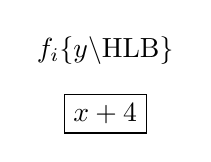
\begin{tikzpicture}[auto]
	% title node
	\node [novertex] (N0) {$f_i\{y \backslash \textnormal{HLB}\}$};

	% place nodes
	\node [terminal, below of=N0, node distance=0.8cm] (N1) {$x + 4$};

	% draw edges

\end{tikzpicture}
}
 
 \vspace{15mm}

 \scalebox{0.8}{
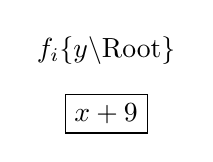
\begin{tikzpicture}[auto]
	% title node
	\node [novertex] (N0) {$f_i\{y \backslash \textnormal{Root}\}$};

	% place nodes
	\node [terminal, below of=N0, node distance=0.8cm] (N1) {$x + 9$};

	% draw edges

\end{tikzpicture}
}
 
 
 \end{minipage}

 \caption{Step 1, 2 and 3 of XADD Continuous Maximization for one case partition: $\phi_i ( x,d,y): f_i$ where $ \phi_i =  d \wedge ( y > 2 ) \wedge ( y < 16) \wedge ( y < x )$  
 and  $f_i =  x -y^2+6y$. (1) Finding the sets UB,LB, Root, and Ind; (2) compute HLB and LUB; and (3) apply the substitution operator $\{y/f\}$, with Root, HLB and LUB.}
 \label{fig:step123:xadd_max}
 \end{figure}
%%%%%%%%%%%%%%%%%%%%

\begin{figure}
% \begin{minipage}{1.0cm}
 \centering
% \rotatebox{-45}{$\rightarrow$}

% \vspace{14mm}

% \rotatebox{45}{$\rightarrow$}
% \end{minipage}
 \begin{minipage}{0.35\linewidth}
 \centering
 \scalebox{0.8}{
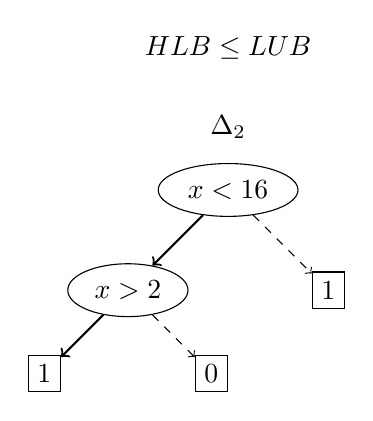
\begin{tikzpicture}[auto]
	% title node
    \node [novertex] (N20) {$HLB \leq LUB $};
	\node [novertex, below of=N20] (N0) {$\Delta_2$};
	% place nodes
	\node [inode, below of=N0, node distance=0.8cm]          (N1) {$x < 16$};
	\node [inode, below left of=N1, node distance=1.8cm]     (N2) {$x > 2$};
    \node [terminal, below right of=N1, node distance=1.8cm]    (N3) {$1$};
	\node [terminal, below left of=N2, node distance=1.5cm]  (N4) {$1$};
	\node [terminal, below right of=N2, node distance=1.5cm] (N5) {$0$};

	% draw edges
    \path [high] (N1) -- (N2);
    \path [low]  (N1) -- (N3);
    \path [high] (N2) -- (N4);
    \path [low]  (N2) -- (N5);
\end{tikzpicture}
}
 \end{minipage}
\begin{minipage}{0.35\linewidth}
 \centering

 \scalebox{0.8}{
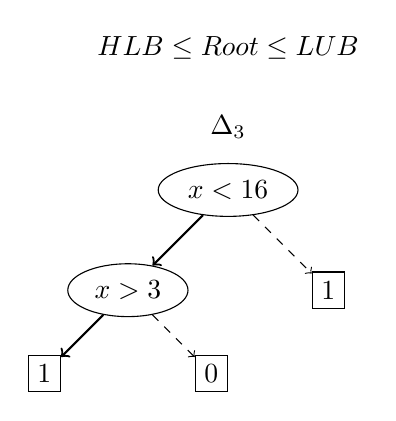
\begin{tikzpicture}[auto]
	% title node
	\node [novertex] (N20) {$HLB \leq Root \leq LUB$};
	\node [novertex, below of=N20] (N0) {$\Delta_3$};
	% place nodes
	\node [inode, below of=N0, node distance=0.8cm]          (N1) {$x < 16$};
	\node [inode, below left of=N1, node distance=1.8cm]     (N2) {$x > 3$};
    \node [terminal, below right of=N1, node distance=1.8cm]    (N3) {$1$};
	\node [terminal, below left of=N2, node distance=1.5cm]  (N4) {$1$};
	\node [terminal, below right of=N2, node distance=1.5cm] (N5) {$0$};

	% draw edges
    \path [high] (N1) -- (N2);
    \path [low]  (N1) -- (N3);
    \path [high] (N2) -- (N4);
    \path [low]  (N2) -- (N5);
\end{tikzpicture}
}

 \end{minipage}
 \caption{Step 4 of XADD Continuous Maximization for one case partition: Compute the conditions $HLB \leq LUB$ and $HLB \leq \Root \leq LUB$.}
\label{fig:step4:xadd_max}
 \end{figure}
%%%%%%%%%%%%%%%%%%%%%%%%%%%%%%
\begin{figure}
 %\begin{minipage}{1.0cm}
 \centering
 %\rotatebox{-45}{$\rightarrow$}

 %\vspace{14mm}

 %\rotatebox{45}{$\rightarrow$}
 %\end{minipage}
 \begin{minipage}{0.35\linewidth}
 \centering
 \scalebox{0.8}{
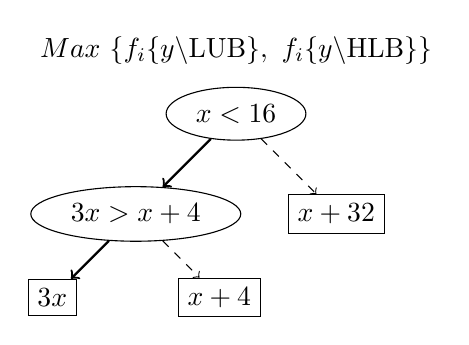
\begin{tikzpicture}[auto]
	% title node
	\node [novertex] (N0) {$Max~\{ f_i\{y\backslash\textnormal{LUB}\},~f_i\{y\backslash\textnormal{HLB}\} \}$};

	% place nodes
	\node [inode, below of=N0, node distance=0.8cm]          (N1) {$x < 16$};
	\node [inode, below left of=N1, node distance=1.8cm]     (N2) {$3x > x+4$};
    \node [terminal, below right of=N1, node distance=1.8cm]    (N3) {$x + 32$};
	\node [terminal, below left of=N2, node distance=1.5cm]  (N4) {$3x$};
	\node [terminal, below right of=N2, node distance=1.5cm] (N5) {$x+4$};

	% draw edges
    \path [high] (N1) -- (N2);
    \path [low]  (N1) -- (N3);
    \path [high] (N2) -- (N4);
    \path [low]  (N2) -- (N5);
\end{tikzpicture}
}
 \end{minipage}
 \begin{minipage}{0.35\linewidth}
 \centering
 \scalebox{0.8}{
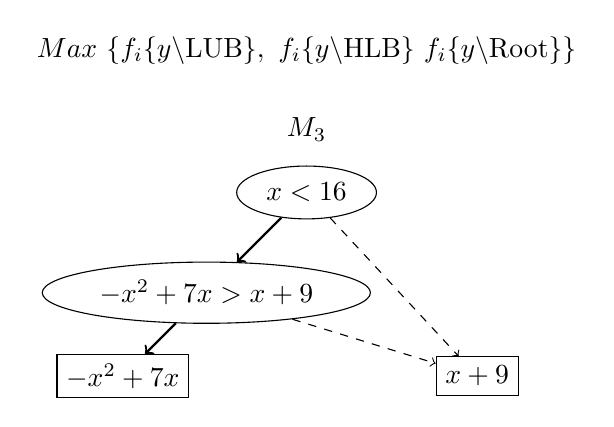
\begin{tikzpicture}[auto]
	% title node
	\node [novertex] (N20) {$Max~\{ f_i\{y\backslash\textnormal{LUB}\},~f_i\{y\backslash\textnormal{HLB}\} ~f_i\{y\backslash\textnormal{Root}\} \}$};
    \node [novertex, below of=N20] (N0) {$M_3$};
	% place nodes
	\node [inode, below of=N0, node distance=0.8cm]          (N1) {$x < 16$};
	\node [inode, below left of=N1, node distance=1.8cm]     (N2) {$-x^2+7x > x+9$};
    %\node [terminal, below right of=N1, node distance=1.8cm]    (N3) {$x + 32$};
	\node [terminal, below left of=N2, node distance=1.5cm]  (N4) {$-x^2+7x$};
	\node [terminal, right of=N4, node distance=4.5cm] (N5) {$x+9$};

	% draw edges
    \path [high] (N1) -- (N2);
    \path [low]  (N1) -- (N5);
    \path [high] (N2) -- (N4);
    \path [low]  (N2) -- (N5);
\end{tikzpicture}
}
 \end{minipage}
 \caption{Step 5 of XADD Continuous Maximization for one case partition: Compute $\casemax$ of the substitutions result.}
\label{fig:step5:xadd_max}
 \end{figure}

\begin{figure}
 \centering
 %\begin{minipage}{0.6cm}
 %\centering
 %\small
% \emph{cons} \\ $+$ \\ \emph{ind} \\
 %$\rightarrow$
 %\end{minipage}
 \begin{minipage}{0.30\linewidth}
 \centering
 \scalebox{0.8}{
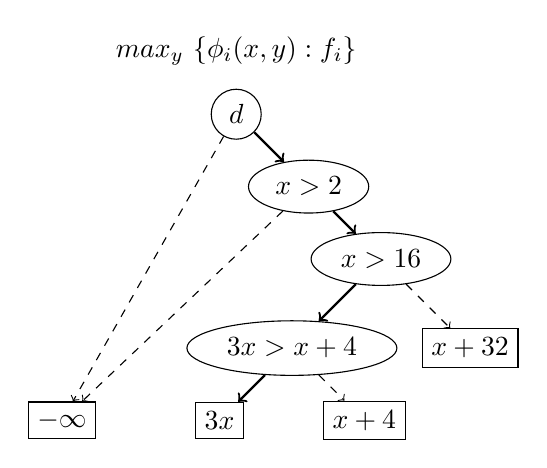
\begin{tikzpicture}[auto]
	% title node
	\node [novertex] (N0) {$max_y~\{\phi_i(x,y) : f_i\}$};

	% place nodes
	\node [root, below of=N0, node distance=0.8cm]           (N1) {$d$};
	\node [inode, below right of=N1, node distance=1.3cm]    (N2) {$x > 2$};
	\node [inode, below right of=N2, node distance=1.3cm]    (N3) {$x > 16$};
	\node [inode, below left of=N3, node distance=1.6cm]     (N4) {$3x > x+4$};
	\node [terminal, below right of=N3, node distance=1.6cm] (N5) {$x+32$};
    \node [terminal, below left of=N4, node distance=1.3cm]  (N6) {$3x$};
    \node [terminal, below right of=N4, node distance=1.3cm] (N7) {$x+4$};
    \node [terminal, left of=N6, node distance=2.0cm]        (N8) {$-\infty$};
    
	% draw edges
    \path [high] (N1) -- (N2);
    \path [high] (N2) -- (N3);
    \path [high] (N3) -- (N4);
    \path [low]  (N3) -- (N5);
    \path [high] (N4) -- (N6);
    \path [low]  (N4) -- (N7);
    
    \path [low] (N1) -- (N8);
    \path [low] (N2) -- (N8);
\end{tikzpicture}
}
 \end{minipage}
 \caption{Step 6 of XADD Continuous Maximization for one case partition: Computing the final result as a new case partition Equation \ref{eq:maxcasepartition}.}
 \label{fig:step6:xadd_max}
 \end{figure}
%\end{landscape}

%%%%%%%%%%%%%%%%%%%%%%%%%%%%%%%%%%%%%%%%%%%%%%%%%%%%%%%%%%%%%%%%%%%%%%%%%%
%\vspace{10mm}
%%\begin{figure}[t!]
%\centering
%\subfigure{
%\hspace{-20mm}
%\vspace{-15mm}
%%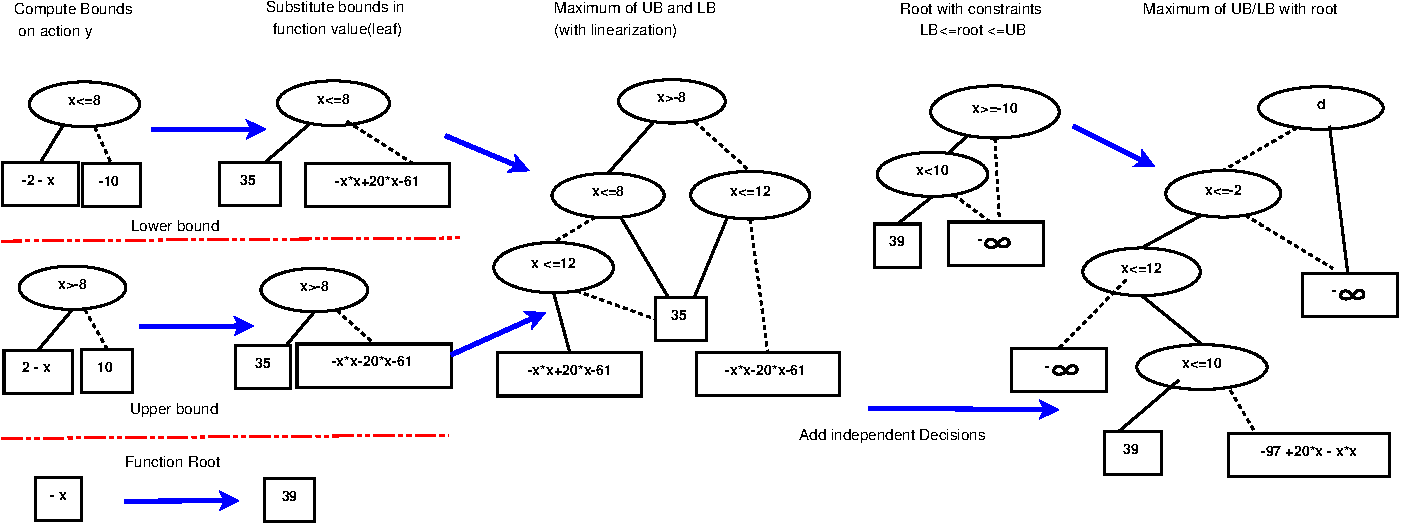
\includegraphics[width=0.97 \textwidth]{pics/maximum_cont_action4.pdf}
%\vspace{-40mm}

%%\caption{%\footnotesize 
%%XADD Continuous Maximization for one state partition:
%%$\phi_i ( x,d,y): f_i$ such $ \phi_i =  d \wedge ( y > 2 ) \wedge ( y < 16) \wedge ( y < x )$  
%%and  $f_i =  x + 2y$.}
%The upper and lower bounds of action $y$ and the root is represented by XADDs and substituted inside the leaf node. The maximum of the upper and lower bound is then represented after linearizing the result. The final result takes the maximum of this and the root considering the constraints and independent decisions.}
%%\label{fig:xadd_max}
%%\end{figure}
%%%%%%%%%%%%%%%%%%%%%%%%%%%%%%%%%%%%%%%%%%%%%%%%%%%%%%%%%%%%%%%%%%%%%%%%%%

\subsubsection{Binary XADD Operations: the Apply algorithm}

%%%%%%%%%%%%%%%%%%%%%%%%%%%%%%%%%%%%%%%%%%%%%%%%%%%%%%%%%%%%%%%%%
\incmargin{0.5em}
\linesnumbered
\begin{algorithm}[t!]
\SetKwInOut{Input}{input}
\SetKwInOut{Output}{output}
\dontprintsemicolon
%\Input{$F_1$ (root node id for operand 1),\\
%$F_2$ (root node id for operand 2)}
%\Output{$var$ (selected variable to branch)}
\Begin{
   //select the decision to branch based on the order\\
   \If{$F^1$ is a terminal node}
    {
     \Return{$\mathit{F^2_{dec}}$}\;  
    }
    \If{$F^2$ is a terminal node}
    {
     \Return{$\mathit{F^1_{dec}}$}\;  
    }
    \eIf{Order($\mathit{F^1_{dec}}) <$ Order($\mathit{F^2_{dec}})$}
	    {
         \Return{$\mathit{F^1_{dec}}$}\;  
	    }
	    {
         \Return{$\mathit{F^2_{dec}}$}\;  
	    }
}
\caption{{\sc ChooseEarliestDec}($F^1,F^2$) $\longrightarrow$ $\langle \mathit{F_{dec}} \rangle$ \label{algChooseDecBranch}}
\end{algorithm}
\decmargin{0.5em}
%%%%%%%%%%%%%%%%%%%%%%%%%%%%%%%%%%%%%%%%%%%%%%%%%%%%%%%%%%%%%%%%%

%%%%%%%%%%%%%%%%%%%%%%%%%%%%%%%%%%%%%%%%%%%%%%%%%%%%%%%%%%%%%%%%%%%%%%%%%%%
\begin{table}[!h]
%\vspace{5mm}
\begin{center}
    \begin{tabular}{|l|l|l|}
	 \hline
	 Input Case & Result \\ \hline \hline
      $F^1\ \mathit{op}\ F^2; F^1=\mathit{Poly}^1; F^2=\mathit{Poly}^2$ & $\mathit{Poly}^1\ \mathit{op}\ \mathit{Poly}^2$ \\
	 \hline
          $F \oplus 0$ or $0 \oplus F$ & $F$\\
	 \hline
         $F  \ominus 0$ & $F$\\
	 \hline
         $F  \otimes 1$ or $1  \otimes F$ & $F$\\
	 \hline
         $F  \otimes 0$ or $0  \otimes F$ & $0$\\
	 \hline
          $F \oplus \infty $ or $\infty \oplus F $ & $\infty$\\
	 \hline
          $F  \otimes +\infty ; F > 0$ or $F  \otimes -\infty ; F < 0$  & $+\infty$\\
      \hline
          $F  \otimes +\infty ; F < 0$ or $F  \otimes -\infty ; F > 0$  & $-\infty$\\
	 \hline
          casemax$(F, +\infty)$ or casemax$(+\infty, F)$  & $+\infty$\\
	 \hline
          casemax$(F, -\infty)$ or casemax$(-\infty, F)$  & $F$\\
	 \hline
	      casemin$(F, +\infty)$ or casemin$(+\infty, F)$  & $F$\\
	 \hline
          casemin$(F, -\infty)$ or casemin$(-\infty, F)$  & $-\infty$\\
           \hline
          casemax $(F^1  , F^2)$, $F^1=Poly^1$ and $F^2=Poly^2$   &\hspace{3mm} 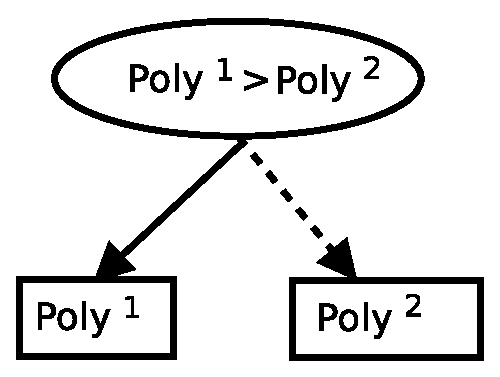
\includegraphics[width=0.20\textwidth]{FiguresSource/max_result.eps}\\
	 \hline
          casemin $(F^1, F^2)$, $F^1=Poly^1$ and $F^2=Poly^2$ &\hspace{3mm}  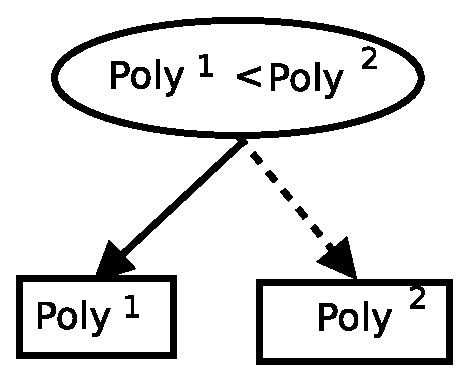
\includegraphics[width=0.20\textwidth]{FiguresSource/min_result.eps}\\
	 \hline
	  other& $\mathit{null}$\\
         \hline
    \end{tabular}
  \caption{\emph{ComputeResult} method: Special input cases and immediate results used in the algorithm \emph{Apply} (Algorithm \ref{algApply}).
  %\footnote{Note that for lines 9--12 the zero case should be tested first.}
  }
  \label{tab:ComputeResultXADD}
\end{center}
\end{table}

For \emph{all} binary operations, the function \emph{Apply}($F^1,F^2,\mathit{op}$) (Algorithm \ref{algApply}) computes the resulting XADD. 
%Table \ref{tab:ComputeResultXADD} which is implemented as a function \emph{ComputeResult} defines the result of XADD operations in special cases to avoid unnecessary computation in \emph{Apply}.
%Any operation with two XADDs, $F_1$ and $F_2$, results in a new canonical XADD $F_r$, with eventually a new root node $F^{var}_r$ and two new sub-diagrams $F_h$ and $F_l$.
The inputs of the algorithm are: two reduced XADD operands $F^1$ and $F^2$ and a binary operator $\mathit{op} \in \{ \oplus, \ominus, \otimes , \max , \min \} $. The output $F^r$ is a reduced XADD after applying the binary operation. 

If the input of Apply algorithm is one of the special cases described in Table  \ref{tab:ComputeResultXADD} (\emph{ComputeResult} method), the result can be immediately computed (without recursion). Otherwise it checks the \emph{ApplyCache} for any previously stored result (Line 6).  If there is not a cache hit, the earliest decision in the XADD ordering is chosen to branch according to Algorithm~\ref{algChooseDecBranch}. Two recursive \emph{Apply} calls are then made on the branches of this decision to compute $F_l$ and $F_h$ (Line 26 and 27). Finally \emph{GetNode} checks for any repeated branches in $F^r$ before storing it in the cache and returning the resulting XADD. 
This algorithm can be described in details using the following steps:

%%%%%%%%%%%%%%%%%%%%%%%%%%%%%%%%%%%%%%%%%%%%%%%%%%%%%%%%%%%%%%%%%
\incmargin{0.5em}
\linesnumbered
\begin{algorithm}[t!]
\SetKwFunction{computeResult}{{\sc ComputeResult}}
\SetKwFunction{Reorder}{{\sc Reorder}}
\SetKwFunction{apply}{Apply} \SetKwFunction{getNode}{{\sc GetNode}}
\SetKwFunction{chooseEarliestDec}{{\sc ChooseEarliestDec}}
\SetKwInOut{Input}{input} \SetKwInOut{Output}{output}
\dontprintsemicolon
%\Input{$F_1$ (root node id for operand 1),\\
%$F_2$ (root node id for operand 2),\\
%$\mathit{op}$ (binary operator, $\mathit{op} \in \{
%\oplus, \ominus, \otimes \}$)}
%\Output{$F_r$ (root node id for the resulting reduced XADD)}
\Begin{
$F^r \leftarrow$ \computeResult{$F^1,F^2,\mathit{op}$} \\  
   //check if the result can be immediately computed in Table   \ref{tab:ComputeResultXADD}\\
   \If{$F^r \neq \mathit{null}$}
      {
      \Return{$F^r$}\;
      }
  $F^r \leftarrow$ \emph{ApplyCache}($\langle F^1,F^2,\mathit{op})\rangle$\\    
   //check if we previously computed the same operation\\
   \If{$F^r \neq$ null}
   {
      \Return{$F^r$}\;
   }   
   //choose decision to branch\\
   $\mathit{F_{dec}} \leftarrow $ \chooseEarliestDec{$F^1,F^2$}\; 
   //set up nodes for recursion\\
   \eIf{$F^1$ is non-terminal $\wedge\ \mathit{F_{dec}}=\mathit{F^1_{dec}}$}
   {
    $F_l^{v1}\leftarrow F^1_{l}$\;
    $F_h^{v1}\leftarrow F^1_{h}$\; 
   }
   {
     $F_l^{v1}\leftarrow F^1$\;
     $F_{h}^{v1}\leftarrow F_{1}$\;
   }
   \eIf{$F^2$ is non-terminal $\wedge\ \mathit{F_{dec}}=\mathit{F^2_{dec}}$}
   {
     $F_l^{v2}\leftarrow F^2_{l}$\;
     $F_h^{v2}\leftarrow F^2_{h}$\; 
   }
   {
     $F_l^{v2}\leftarrow F^2$\;
     $F_{h}^{v2}\leftarrow F_{2}$\;
   }
   //use recursion to compute true and false branches for resulting XADD\\
   $F_l\leftarrow $ \apply{$F_l^{v1},F_l^{v2},\mathit{op}$}\;    
   $F_h\leftarrow $ \apply{$F_h^{v1},F_h^{v2},\mathit{op}$}\; 
   $F^r\leftarrow $ \getNode{$\mathit{F_{dec}},F_h,F_l$}\;
    //Use Algorithm~\ref{alg:reorder} to reorder decisions if necessary\\
   \If{op=casemax or op=casemin}
   { 
   $F^r \leftarrow$ \Reorder{$F^r$}\;
   }
   //save the result to reuse in the future\\
   ApplyCache$(\langle F^1,F^2,\mathit{op}\rangle) \leftarrow F^r$ \;
   \Return{$F^r$}\;
}
\caption{{\sc Apply}($F^1,F^2,\mathit{op}$) $\longrightarrow$ $\langle F^r \rangle$ \label{algApply}}
\end{algorithm}
\decmargin{0.5em}
%%%%%%%%%%%%%%%%%%%%%%%%%%%%%%%%%%%%%%%%%%%%%%%%%%%%%%%%%%%%%%%%%
\begin{itemize}
\item \textbf{Terminal computation}: 
The function \emph{ComputeResult} called in Line 2 determines if the result can be computed without recursion using the pruning optimization described in Table \ref{tab:ComputeResultXADD}. For the discrete maximization (minimization) operation, for two leaf nodes $poly^1$ and $poly^2$ an additional decision node $poly^1 > poly^2$ ($poly^1 < poly^2$) is introduced to represent the maximum (minimum). Note that, this may cause out-of-order decisions which will be reordered by Algorithm~\ref{alg:reorder}. 

\item \textbf{Caching}:
If the result of \emph{ComputeResult} is null, we check the \emph{ApplyCache} in Line 6 for any previously computed operation using these operands and operation. To increase the chance of a match, all items stored in a cache are reduced XADDs.

\item \textbf{Recursive computation}:
If a call to \emph{Apply} is unable to immediately compute a result or reuse a previously cached computation, we must recursively compute the result (Lines 10-28). Since the \emph{ComputeResult} takes care of the case when both operands are terminal nodes, we know that at least one of them is a decision node so one of the following conditions applies: 
\begin{itemize}
\item $F^1$ or $F^2$ is a terminal node or $\mathit{F^1_{dec}}\neq \mathit{F^2_{dec}} $: One of the decision nodes is chosen (e.g. $F^2$) by 
\emph{ChooseEarliestDec} method and two recursive \emph{Apply} calls are performed using its corresponding branches ($F^2_{h}$ and 
$F^2_{l}$) with the other operand (e.g., $F^1$).
The result of these two \emph{Apply} functions is used with the decision $\mathit{F^2_{dec}}$ for a reduced result:
\begin{align*}
F_h & \leftarrow Apply (F^1 , F^2_{h},op) \\
F_l & \leftarrow Apply (F^1 , F^2_{l},op)  \\
F^r & \leftarrow GetNode (\mathit{F^2_{dec}} , F_h,F_l) 
\end{align*}
\item $F^1$ and $F^2$ are decision nodes and $\mathit{F^1_{dec}}=\mathit{F^2_{dec}} $: Since the decisions are equal, the final result is a decision with the constraint $\mathit{F^1_{dec}} (=\mathit{F^2_{dec}})$; the high branch is obtained by calling \emph{Apply} on $F_h^1$ and $F_h^2$ and the low branch is the result of the \emph{Apply} function on $F_l^1$ and $F_l^2$, i.e.:
\begin{align*}
F_h & \leftarrow Apply (F^1_{h} , F^2_{h},op)  \\
F_l & \leftarrow Apply (F^1_{l} , F^2_{l},op)  \\
F^r & \leftarrow GetNode (\mathit{F^1_{dec}} , F_h,F_l) 
\end{align*}
\end{itemize}
\end{itemize}
Finally the result is a reduced XADD returned by \emph{GetNode} where the decisions are ordered by algorithm \emph{Reorder} if the operation is op=casemax or op=casemin. 

\subsection{Inconsistency and Redundancy Prunning}

%\subsection{Inconsistent Path Formula and Redundant Node}

One issue with applying operations on XADDs is the introduction of redundant nodes or nodes that result in inconsistent path formula (Section \ref{xaddformal}). Therefore after applying any operation on the XADD, it should be checked for any sources of infeasibility so that inconsistent branches are removed and not expanded in later stages. Furthermore, there may be redundant structures in the XADD which result in unnecessary nodes.
Thus, removing redundant nodes from the XADD is also a requirement for obtaining a minimal XADD representation. 






%%%%%%%%%%%%%%%%%%%%%%%%%%%%%%%%%%%%%%%%%%%%%%%%%%%%%%%%%%%%%%%%%%%%%%%%%%%%
%\vspace{10mm}
\begin{figure}[t!]
\centering
%\subfigure{
%\hspace{-20mm}
%\vspace{-3mm}
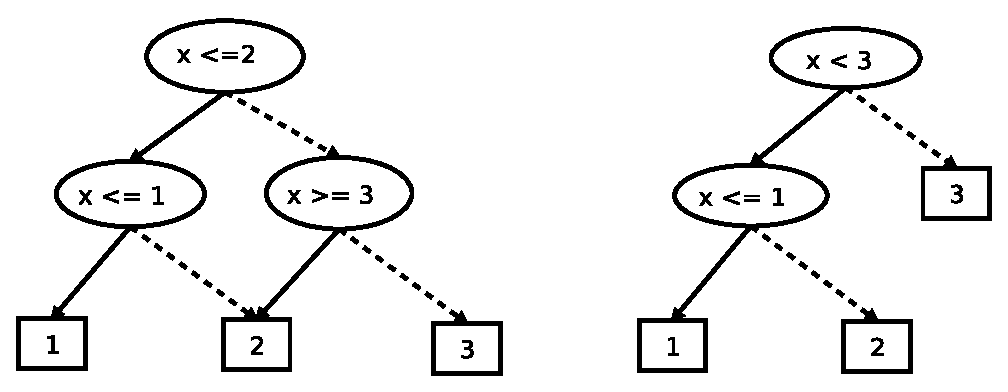
\includegraphics[width=0.6\textwidth]{FiguresSource/counterExample.eps} 
%\hspace{20mm}
%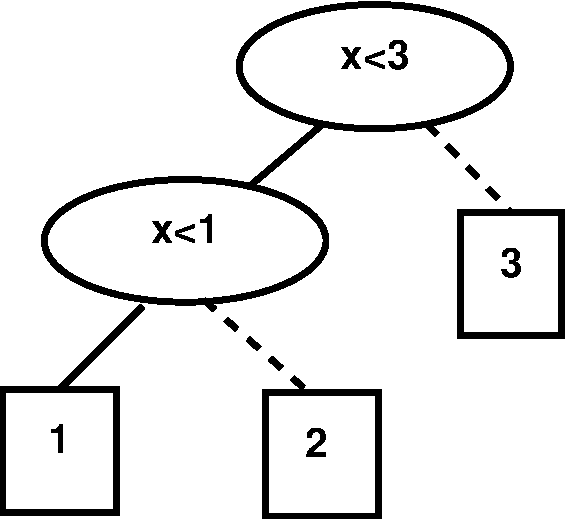
\includegraphics[width=0.28\textwidth]{pics/counterexample2.pdf} 
%\includegraphics[width=0.62\textwidth]{xaddFig/redundancy_proof.pdf}
\caption{%\footnotesize 
{\it (left)} A counterexample for an XADD that is not canonical after applying consistency and redundancy checking; {\it (right)}  The minimal XADD which can not be derived from the left diagram.  \color{red}  TODO: Trocar na figura o nó $x>=3$ por $x<3$. } %{\it (right)} Example of removing the redundant node $i$ which must result in an equal XADD from root up to node $i$ branched on the true or false branch of $dec_i$. }
\label{fig:canonical}
%\vspace{-6mm}
\end{figure}
%%%%%%%%%%%%%%%%%%%%%%%%%%%%%%%%%%%%%%%%%%%%%%%%%%%%%%%%%%%%%%%
%%%added after taking canonical proof out


In this section we  provide efficient algorithms to prune linear XADDs (currently we don't have efficient algorithms to prune XADDs with nonlinear decisions). 

%\subsection{Inconsistency and Redundancy Prunning Algorithms}
%\label{sec:pruningAlg}

%%%%%%%%%%%%%%%%%%%%%%%%%%%%%%%%%%%%%%%%%%%%%%%%%%%%%%%%%%%%%%%%
\incmargin{.5em}
\linesnumbered
\begin{algorithm}[t!]
\SetKwFunction{getNode}{{\sc GetNode}}
\SetKwFunction{testImplied}{{\sc TestImplied}}
\SetKwFunction{prune}{{\sc PruneInconsistent}}
\SetKwFunction{pruneRedu}{{\sc PruneRedundant}}
\SetKwFunction{redundant}{{\sc IsRedundant}}
\SetKwInOut{Input}{input}
\SetKwInOut{Output}{output}
\dontprintsemicolon
%\Output{$F_r$ (root node id for a consistent XADD)}
\BlankLine
\Begin{
    //$F$ is the root node represented as ($F_\mathit{dec},F_h,F_l$)\\
    %//$\psi$ is the set of decision constraints\\
   \If{$F$ is terminal node}
   {
    \Return{canonical terminal node for $F$}\;
   }
   //if $F$ is a boolean decision, no inconsistency checking possible for $F$\\
   \If {$F \in \lbrace 0,1 \rbrace^m$}
   {
    $low \leftarrow $  \prune{$F_l$, $\psi$}\;
    $high \leftarrow $  \prune{$F_h$, $\psi$}\;	
    \Return  {\getNode{$F_\mathit{dec},high,low$}}\; 
   }
   //else $F$ is a linear decision check if  $\psi\models\perp$\\
   
    	 \If{\testImplied{$\psi$,$F_\mathit{dec}$}}
    			{ \Return { \prune{$F_h$, $\psi$}}\;}
    	 \If{\testImplied{$\psi$,$\neg F_\mathit{dec}$}}
    			{\Return { \prune{$F_l$, $\psi$}}\;}
  //result of TestImplied was false then prune both branches\\
    $low\leftarrow $  \prune{$F_l$, $\psi \wedge \neg F_\mathit{dec}$}\;
    $high\leftarrow $  \prune{$F_h$, $\psi \wedge  F_\mathit{dec}$}\;	 
     // return the new XADD with the pruned branches\\
   \Return{\getNode{$F_\mathit{dec},high,low$}}\;
}
\caption{{\sc PruneInconsistent}($F$, $\psi$) $\longrightarrow$ $\langle F^r \rangle$ \label{algPrune}}
\end{algorithm}
\decmargin{.5em}
%%%%%%%%%%%%%%%%%%%%%%%%%%%%%%%%%%%%%%%%%%%%%%%%%%%%%%%%%%%%%%%%%

%%%%%%%%%%%%%%%%%%%%%%%%%%%%%%%%%%%%%%%%%%%%%%%%%%%%%%%%%%%%%%%%
\incmargin{.5em}
\linesnumbered
\begin{algorithm}[t!]
\SetKwFunction{getNode}{{\sc GetNode}}
\SetKwFunction{testImplied}{{\sc TestImplied}}
\SetKwFunction{prune}{{\sc PruneRedundant}}
\SetKwFunction{redundant}{{\sc IsRedundant}}
\SetKwInOut{Input}{input}
\SetKwInOut{Output}{output}
\dontprintsemicolon
%\Output{$F_r$ (root node id for a consistent XADD)}
\BlankLine
\Begin{
    //$F$ is the root node represented as ($F_\mathit{dec},F_h,F_l$)\\
     //check if high branch is implied in the low branch for $F_\mathit{dec}$\\
     $\mathit{isRedundant} = $\redundant{$\psi \wedge F_\mathit{dec}$,$F_l$, $F_h$}\;
     \If {$\mathit{isRedundant}$}
    {\Return{\prune{$F_\mathit{l}$, $\psi$}}\;}     
	//check if low branch is implied in the high branch for $\neg F_\mathit{dec}$\\
	 $\mathit{isRedundant} = $\redundant{$\psi \wedge \neg F_\mathit{dec} $,$F_h$, $F_l$}\;
       \If {$\mathit{isRedundant}$}
    {\Return{\prune{$F_\mathit{h}$, $\psi$}}\;}
    //return the new XADD with the pruned branches\\
    $low \leftarrow$ \prune{$F_\mathit{l}$, $\psi \wedge \neg F_\mathit{dec}$} \;
    $high \leftarrow$ \prune{$F_\mathit{h}$, $\psi \wedge  F_\mathit{dec}$} \;
    \Return{\getNode{$F_\mathit{dec},high,low$}}\;
}
\caption{{\sc PruneRedundant}($F$, $\psi$) $\longrightarrow$ $\langle F^r \rangle$ \label{algPruneRedundant}}
\end{algorithm}
\decmargin{.5em}
%%%%%%%%%%%%%%%%%%%%%%%%%%%%%%%%%%%%%%%%%%%%%%%%%%%%%%%%%%%%%%%%%

% Figures used for the inconsistency and redundancy prunning algorithms  
%
%%%%%%%%%%%%%%%%%%%%%%%%%%%%%%%%%%%%%%%%%%%%%%%%%%%%%%%%%%%%%%%%%%%%%%%%%%
\begin{figure}[t!]
\centering
%\subfigure{
%\hspace{-20mm}
%\vspace{-3mm}
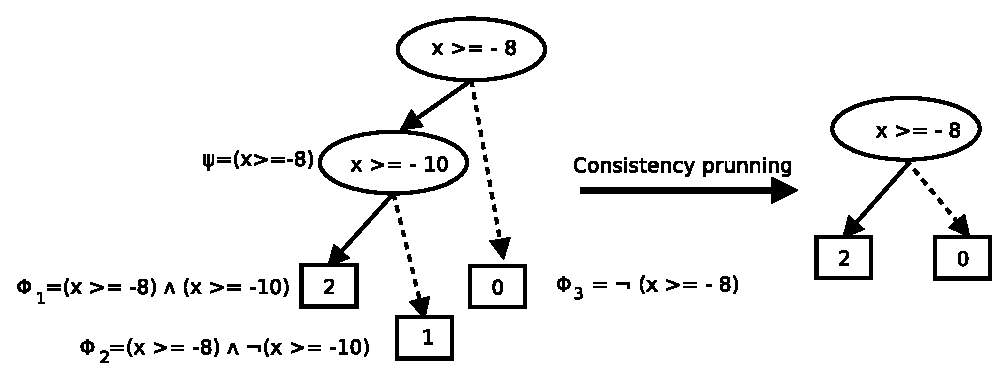
\includegraphics[width=0.8\textwidth]{FiguresSource/consistencyPrunning.eps}
% * <karinaval@gmail.com> 2016-04-18T13:42:42.245Z:
%
% > Prunning
%
% ^.
%\vspace{-3mm}
%\hspace{1mm}
%\includegraphics[width=0.18\textwidth]{xaddFig/counterexample.pdf}
\vspace{-2mm}
\caption{%\footnotesize 
XADD with an Inconsistent Path Formula:  {\it (left)} Path definitions on each node in the XADD with an inconsistent path formula $\psi(n_1, n_2, n_4)$, i.e. $((x \geq -8) \wedge \neg (x \geq -10) \models\perp)$; {\it (right)} Pruned XADD after removing path $C=(n_1, n_2, n_4)$. Note that $n_4$ is unreachable and then removed; consequently $n_2$ is an unnecessary decision and it is also removed. 
}
\label{fig:consistent_graph}
%\vspace{-4mm}
\end{figure}


\begin{figure}[t!]
\centering
%\subfigure{
%\hspace{-20mm}
%\vspace{-3mm}
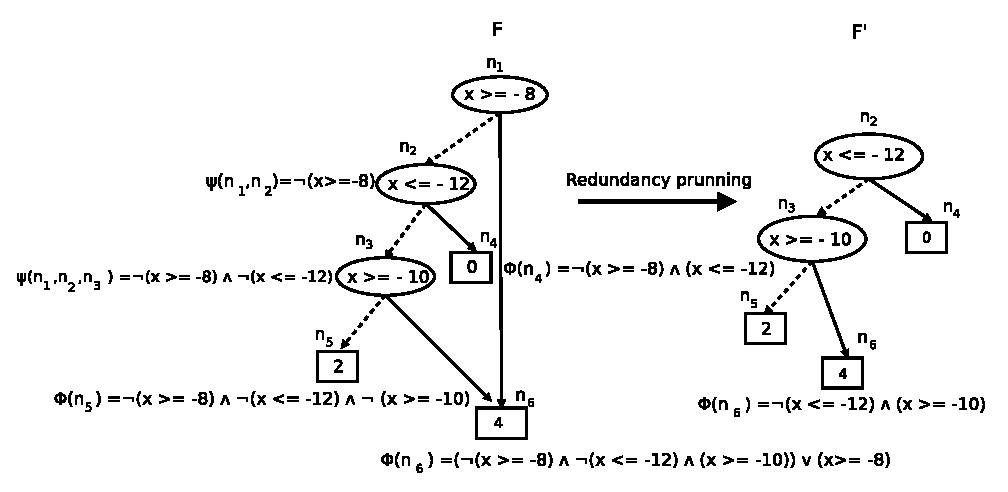
\includegraphics[width=1\textwidth]{FiguresSource/redundancyPrunning.eps}
%\vspace{-3mm}
%\hspace{1mm}
%\includegraphics[width=0.18\textwidth]{xaddFig/counterexample.pdf}
\vspace{-2mm}
\caption{%\footnotesize 
XADD with a Redundant Node:  {\it (left)} Path definitions on each node in the XADD with a redundant node $n_1$  ($x>=-8$). It is redundant since $n_2$ represents the same function as $n_1$; (right) The pruned XADD F without the redundant node $n_1$. Note that all leaf nodes $n_i$ have the same partition, i.e. $\phi(n_i) \equiv \phi'(n_i)$.}
\label{fig:redundant_graph}
%\vspace{-4mm}
\end{figure}
%%%%%%%%%%%%%%%%%%%%%%%%%%%%%%%%%%%%%%%%%%%%%%%%%%%%%%%%%%


\subsubsection{Inconsistency Pruning Algorithm}

Given a linear XADD $F$ with possibly inconsistent paths and the set of decision constraints on a path $\psi$, the output of \emph{PruneInconsistent} (Algorithm~\ref{algPrune}) is a reduced XADD with canonical leaves, linear decisions and no unreachable nodes. Similar to Algorithm \emph{Reduce-XADD}, this algorithm is of a recursive bottom-up nature. 

Lines 3--4 of Algorithm~\ref{algPrune} return a canonical linear expression at the leaf if $F$ is a terminal node. Since $F$ does not require path consistency checking at a boolean decision node. Lines 6--9 recursively calls inconsistency pruning on the low and high branches. The final result is returned using Algorithm \emph{GetNode}.

If the two mentioned conditions are false, then the current node of $F$ is a linear decision node. In this case, we check if the decision test of this node ($F_\mathit{dec}$) is consistent with the previous constraints on path $\psi$. 
Algorithm~\ref{algPrune}, Lines 11 and 13 use the \emph{TestImplied} function (Algorithm \ref{algTestImplied}) that has a  path formula  $\psi$ and current decision test $F_\mathit{dec}$ as inputs. This function performs the following steps:

\begin{itemize}
\item Check if the implication result of $\psi$ exists in an \emph{Implications} cache. This cache stores path formulas $\psi$ that are inconsistent. If there is a previous result which already contains the new decision constraint $F_\mathit{dec}$ then return $\mathit{true}$.
\item Similarly check the \emph{non-Implications} cache for consistent path formulas $\psi$. If there is a previous result which already contains the new decision constraint $F_\mathit{dec}$ then return $\mathit{false}$.
\item If there is no cache hit, then $F_\mathit{dec}$ is added to the path: $\psi \longleftarrow \psi \wedge \neg F_\mathit{dec}$. This allows us to check for the infeasibility property.
\item The LP-solver is called on the set of decision constraints in $\psi$. The result of the LP-solver determines infeasibility with respect to the new decision just added to $\psi$. 
\item The path $\psi$ is stored in its related cache according to the result of the LP-solver (i.e. $\mathit{true}$ or $\mathit{false}$). If the result is inconsistent then $\psi$ is added to \emph{Implications}, else it is added to \emph{non-Implications}.
% \item The negation of $F_\mathit{dec}$ is removed from the path: $\psi \longleftarrow \psi \setminus \neg F_\mathit{dec}$.
\item TestImplied returns the result of the LP-solver.
\end{itemize}

%%%%%%%%%%%%%%%%%%%%%%%%%%%%%%%%%%%%%%%%%%%%%%%%%%%%%%%%%%%%%%%%
\incmargin{.5em}
\linesnumbered
\begin{algorithm}[t!]
\SetKwFunction{getNode}{{\sc GetNode}}
\SetKwFunction{testImplied}{{\sc TestImplied}}
\SetKwFunction{prune}{{\sc PruneInconsistent}}
\SetKwFunction{pruneRedu}{{\sc PruneRedundant}}
\SetKwFunction{isfeasible}{{\sc IsFeasible}}
\SetKwInOut{Input}{input}
\SetKwInOut{Output}{output}
\dontprintsemicolon
%\Output{$F_r$ (root node id for a consistent XADD)}
\BlankLine
\Begin{
    $\psi \leftarrow \psi \wedge \neg F_{dec}$\;
    inconsistent $\leftarrow$ ImplicationCache($\psi$)\;
    \If{inconsistent $\neq$ null}
   {
    \Return{true}\;
   }
    consistent $\leftarrow$ NonImplicationCache($\psi$)\;
    \If{consistent $\neq$ null}
   {
    \Return{false}\;
   }
    \eIf{LPSolve.\isfeasible{$\psi$}}
   {
    NonImplicationCache($\psi$) $\leftarrow$ true \; 
    \Return{false}\;
   }
   {
   ImplicationCache($\psi$) $\leftarrow$ true \; 
    \Return{true}\;
   }   
}
\caption{{\sc TestImplied}($\psi$, $F_{dec}$)  \label{algTestImplied}}
\end{algorithm}
\decmargin{.5em}
%%%%%%%%%%%%%%%%%%%%%%%%%%%%%%%%%%%%%%%%%%%%%%%%%%%%%%%%%%%%%%%%%


Line 11 of Algorithm \ref{algPrune} checks if the true assignment of $F_\mathit{dec}$ is implied by $\phi$. If   \emph{TestImplied} is $\mathit{true}$, then the low branch is inconsistent and the algorithm returns the high branch as the result of this pruning (Line 12). Similarly in Line 13 $\neg F_\mathit{dec}$ is checked and if \emph{TestImplied} is $\mathit{true}$ then the high branch is inconsistent and the low branch returned after pruning (Line 14). 

In case the current decision node is not an inconsistent path, both low and high branches need to be checked for inconsistency. Line 16 adds the decision constraint $\neg F_\mathit{dec}$ to $\psi$ and call \emph{PruneInconsistent} for $F_l$. Line 17 performs the same for the high branch ($F_h$) adding $F_\mathit{dec}$. At this stage the current subtree with the computed low and high branches does not contain any inconsistent paths. Thus the algorithm returns a reduced node computed using \emph{GetNode} in Line 19. 
%%%%%%%%%%%%%%%%%%%%%%%%%%%%%%%%%%%%%%%%%%%%%%%%%%%%%%%%%%%%%%%%%
\incmargin{.5em}
\linesnumbered
\begin{algorithm}[t!]
\SetKwFunction{getNode}{{\sc GetNode}}
\SetKwFunction{testImplied}{{\sc TestImplied}}
\SetKwFunction{prune}{{\sc IsRedundant}}
\SetKwInOut{Input}{input}
\SetKwInOut{Output}{output}
\dontprintsemicolon
%\Input{$X$ (root node id for a consistent XADD), $KB$ (child-parent implications), $F$ (formulas for each node)}
\BlankLine
\Begin{
	\If{$\mathit{subtree} = \mathit{goal}$}
   {
    \Return{$\mathit{true}$}\;
   }
   // a terminal node can not achieve goal\\
   \If{$\mathit{subtree}$ is a terminal node}
   {
    \Return{$\mathit{false}$}\;
   }
   	   \If{$\mathit{goal}$ is non-terminal node}
       {
    	   //node is not redundant if the goal occurs before subtree in the XADD order\\
    	   \If{$\mathit{Order(subtree}_{\mathit{dec}}) \geq \mathit{Order(goal}_{\mathit{dec}}$)}
    	    {
   				 \Return{$\mathit{false}$}\;
   			}
       }
       	// check if $\mathit{subtree}_{\mathit{dec}}$ is implied by $\psi$ to prune search\\
        \If{\testImplied{$\psi$,$\neg \mathit{subtree}_{\mathit{dec}}$}}
    			{ \Return { \prune{$\psi$,$\mathit{subtree}_l$ ,$\mathit{goal}$}}\;}
    	 \If{\testImplied{$\psi$,$\mathit{subtree}_{\mathit{dec}}$}}
    			{\Return { \prune{$\psi$,$\mathit{subtree}_h$ ,$\mathit{goal}$}}\;}      
      //result of TestImplied was false\\
      $\mathit{isImplied} \leftarrow$  \prune{$\psi \wedge \neg \mathit{subtree}_{\mathit{dec}}$,$\mathit{subtree}_l$ ,$\mathit{goal}$}\;
    //if the low branch does not imply goal, the node is not redundant\\
     \If{$\neg \mathit{isImplied}$}
    	    {
   				 \Return{$\mathit{false}$}\;
   			}
$\mathit{isImplied} \leftarrow$  \prune{$\psi \wedge \mathit{subtree}_{\mathit{dec}}$,$\mathit{subtree}_h$ ,$\mathit{goal}$}\;
    \Return{$\mathit{isImplied}$}\;		
}
\caption{{\sc IsRedundant}($\psi$, $\mathit{subtree}$, $\mathit{goal}$) $\longrightarrow$ $\langle \mathit{true}, \mathit{false} \rangle$ \label{algRedundant}}
\end{algorithm}
\decmargin{.5em}
%%%%%%%%%%%%%%%%%%%%%%%%%%%%%%%%%%%%%%%%%%%%%%%%%%%%%%%%%%%%%%%%%
\subsubsection{Redundancy Pruning Algorithm}
\label{redundancyprunning}

The algorithm \emph{isRedundant} directly checks if a node $F$ can be replaced by the \emph{subtree} branch. It receives a path formula $\psi$ and two XADD nodes, \emph{subtree} and \emph{goal}, and checks if the node \emph{goal} is necessarily achieved in the XADD \emph{subtree} when $\psi$ is true. If the goal node is not achieved in some branch of \emph{subtree}, then the replacement can not be done. 

Initially Lines 2-3 of Algorithm \ref{algRedundant} check if $\mathit{subtree}$ and $\mathit{goal}$ are equal, in this case the node $F$ is redundant and it can be replaced by $\mathit{subtree}$, therefore the algorithm returns $\mathit{true}$. If the nodes are different then the node $F$ is not redundant and Line 6 returns $\mathit{false}$. Next Lines 7--10 check if both nodes are decision nodes but the $\mathit{goal}$ node appears before the $\mathit{subtree}$ in the variable ordering of the XADD, in which case the $\mathit{goal}$ can not be achieved in $\mathit{subtree}$. 

If neither of the above cases occur, the algorithm must search a goal node in the branches of $\mathit{subtree}$. In Lines 12-16 the method \emph{TestImplied} is used to check if the path formula $\psi$ implies $subtree_{dec}$ to restrict the search in one of the branches.   

Similar to Algorithm~\ref{algPrune}, if the result of \emph{TestImplied} is false, both low and high branches need to be checked for redundancy. Line 18 calls the method \emph{IsRedundant} for $\mathit{subtree}_l$ and the path formula $\psi \wedge \neg subtree_{dec}$. Similarly, Line 22 calls \emph{IsRedundant} for $\mathit{subtree}_h$ and the path formula $\psi \wedge subtree_{dec}$. If any of the branches along the way do not imply $\mathit{goal}$, then the node is not redundant and the algorithm returns false. 

The method \emph{PruneRedundant} (Algorithm \ref{algPruneRedundant}) removes any redundant nodes from an XADD F and its corresponding path formula (the path from the root to node F). According to the definition, a node is redundant if it represents the same function as one of its branches. For a \emph{subtree} be used to replace a father node, it must contain it sibling node to achieve the same values in the corresponding regions. In Line 4 of Algorithm \ref{algPruneRedundant}, the method checks if the node $F_l$ can replace the node F. If \emph{isRedundant} returns true, \emph{PruneRedundant} returns the low branch, after a recursive pruning (Line 6); else we check if $F_h$ can replace the node F (Line 8) and, again, if successful returns a high branch after a recursive pruning (Line 10). If the current node is not redundant, we recursively prune both branches (Line 12-13) and return the new node (Line 14). 

Figure~\ref{fig:redundant_graph} shows that the node $x\geq -8$ in the left (where $n_2$ is the subtree and $n_6$ is the goal node in the successful call of the \emph{isRedundant} method) is redundant and can be removed from the original XADD. 

It seems that using the two mentioned pruning techniques of inconsistency and redundancy checking removes all sources of infeasibility and therefore proof of canonicity is straightforward. Indeed for BDDs and ADDs proof of canonicity can be defined using the reduced diagrams \cite{bryant}. 
As we have defined, reduced XADDs are derived from the result of the applying redundant branch pruning.  However unlike BDDs and ADDs a canonical XADD may not be produced after such pruning approaches. As a counterexample consider the simple XADD in  Figure~\ref{fig:canonical} (left) where the values are as follows: 
\begin{align}
\label{redu}
	\begin{cases}
		x \leq 1 :& 1  \\
		x \geq 3 :&3\\
		1<x<3 :& 2\\
	\end{cases}
\end{align}
As the values suggest, there is no need to branch on $x<2$ in this function, i.e. it can be removed from the tree. According to the implication checks in both pruning techniques, this XADD is not inconsistent and further the node $x<2$ can not be removed using the redundant technique which replaces a redundant node with one of its branches. This type of redundant node can be removed with the redundant technique by reordering the decisions in the XADD. For this reason, although consistency and redundancy checking takes care of most unwanted branches, there is no guarantee that a given XADD is minimal after applying the two pruning techniques. The right diagram of Figure~\ref{fig:canonical} is the minimal XADD  for the function described in Equation \ref{redu}. Thus a challenging open problem is the proof of XADD minimality with respect to a given order of the linear decisions. 

%%%%%%%%%%%%%%%55
Having defined the efficient representation of XADDs, next we show results from implementing an SDP algorithm using XADDs.

\section{Experimental Results} \label{results}

We implemented two versions of our proposed SVI algorithms using XADDs one for DA-HMDP and other for CA-HMDP.
% we compare that does not prune nodes of the XADD and another that uses a linear programming solver to prune unreachable nodes (for problems with linear XADDs) and then performs a satisfiability check to prune redundant paths  --- and tested these algorithms on different problems.
For CA-HMDPs we evaluated SVI on a didactic quadratic
\MarsRover\ domain and two problems from the \InventoryControl\ domain defined in the introduction, and \WaterReservoir domain. For comparison purposes, these domains are discretized by their action space to generate DA-HMDP. \footnote{All Java source code and a human/machine readable file format for all domains needed to reproduce
the results in this paper can be found online at
\texttt{https://github.com/ssanner/xadd-inference}.}

\subsection{Domains}

\paragraph{\InventoryControl}
The inventory problem mentioned in the introduction is revisited to compare 1-item, 2-item and 3-item inventories for both deterministic and stochastic customer demands. 
\paragraph{\MarsRover}
A \MarsRover state consists of its continuous position $x$ along a given route.  In a given time step, the rover may move a continuous distance $\Delta x \in [-10,10]$.  The rover receives its greatest reward for taking a picture at $x=0$, which quadratically decreases to zero at the boundaries of the range $x \in [-2,2]$.  The rover will
automatically take a picture when it starts a time step within the range $x \in [-2,2]$ and it only receives this reward once.

Using boolean variable $tp \in \{0,1\}$ to indicate if the picture has
already been taken ($tp=1$), $x'$ and $tp'$ to denote 
post-action state, and $R$ to denote reward, we 
express the \MarsRover\ CA-HMDP using piecewise dynamics and reward:
%\vspace{-4mm}
\begin{align*} 
\hspace{-2.8mm} P(tp'\sq=\sq1|x,tp) & = 
\begin{cases}
tp \lor (x \geq -2 \land x \leq 2): & \sqm 1.0\\
\neg tp \land (x < -2 \lor x > 2):  & \sqm 0.0
\end{cases}  \\
\hspace{-2.8mm} P(x'|x,\Delta x) & = \delta \left( x' - \begin{cases}
\Delta x \geq -10 \land \Delta x \leq 10 : & \hspace{-2mm} x + \Delta x \\
\Delta x < -10 \lor \Delta x > 10 : & \hspace{-2mm} x
\end{cases}
\right)  \\
\hspace{-2.8mm} R(x,tp) & = \begin{cases}
\neg tp \land x \geq -2 \land x \leq 2 : & 40 - x^2 \\
tp \lor x < -2 \lor x > 2 : & -1
\end{cases} 
\end{align*}
%%%%%%%%%%%%%%%%%%%%%%%%%%%%%%%%%%%%%%%%%%%%%%%%%%%%%%%%%%%%%%%%%%%%%%%%%%
%OBS: Figure 13: contrary to what is written in its caption, for V^2 the rover achieves nonzero value up to x=+-18 instead of x=+-22 (analogous for V^1

\begin{figure}[t!]
\centering
\begin{minipage}[b]{1\linewidth}
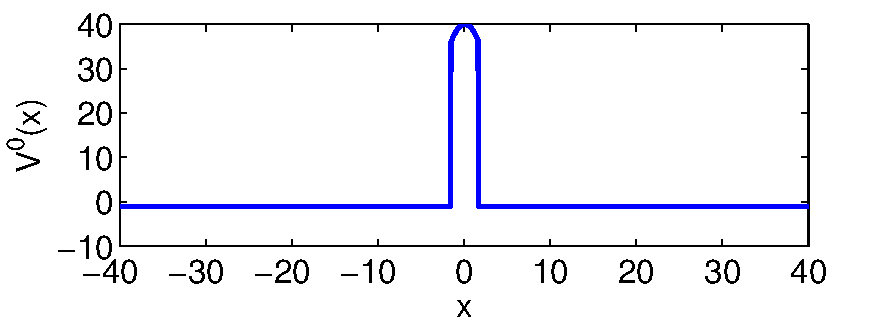
\includegraphics[width=0.5\textwidth]{pics/v1_2d.pdf}
%\vspace{-2mm}
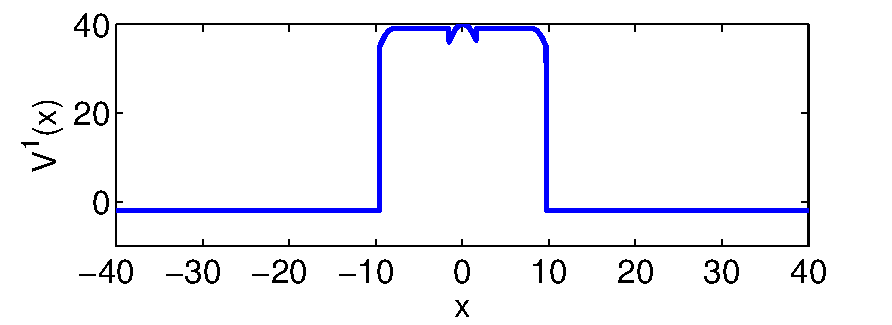
\includegraphics[width=0.5\textwidth]{pics/v2_2d.pdf}\\
%\vspace{-2mm}
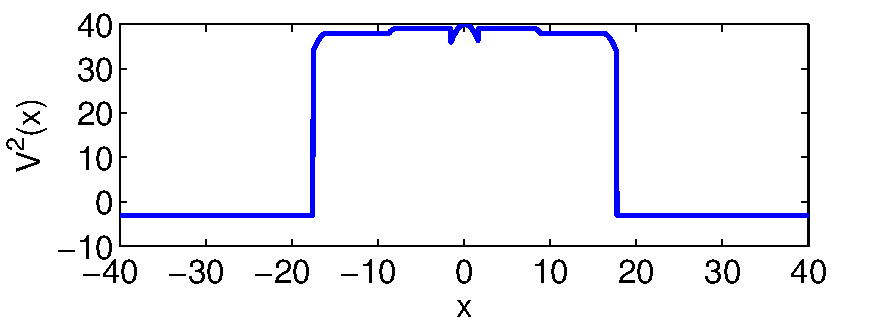
\includegraphics[width=0.5\textwidth]{pics/v3_2d.pdf}
%\vspace{-3mm}

%\parbox{2.8in}{
\caption{Optimal sum of rewards (value) 
$V^t(x)$ for $tp = 0 \, 
(\false)$ for time horizons (i.e., decision stages remaining) $t=0$,
$t=1$, and $t=2$ on the \textsc{Continuous Action}  \MarsRover\ problem.  For $x \in [-2,2]$, the
rover automatically takes a picture and receives a reward quadratic in
$x$.  We initialized $V^0(x,tp) = R(x,tp)$; for $V^1(x)$, the rover achieves
non-zero value up to $x = \pm 12$ and for 
$V^2(x)$, up to $x = \pm 22$.}
\label{fig:opt_graph}

\end{minipage}
\end{figure}
%%%%%%%%%%%%%%%%%%%%%%%%%%%%%%%%%%%%%%%%%%%%%%%%%%%%%%%%%%%%%%%%%%%%%%%%%%
%%%%%%%%%%%%%%%%%%%%%%%%%%%%%%%%%%%%%%%%%%%%%%%%%%%%%%%%%%%%%%%%%%%%%%%%%%
\begin{figure}[t!]
\centering
%\subfigure{
%\hspace{-1mm}
%\begin{minipage}[b]{1\linewidth}
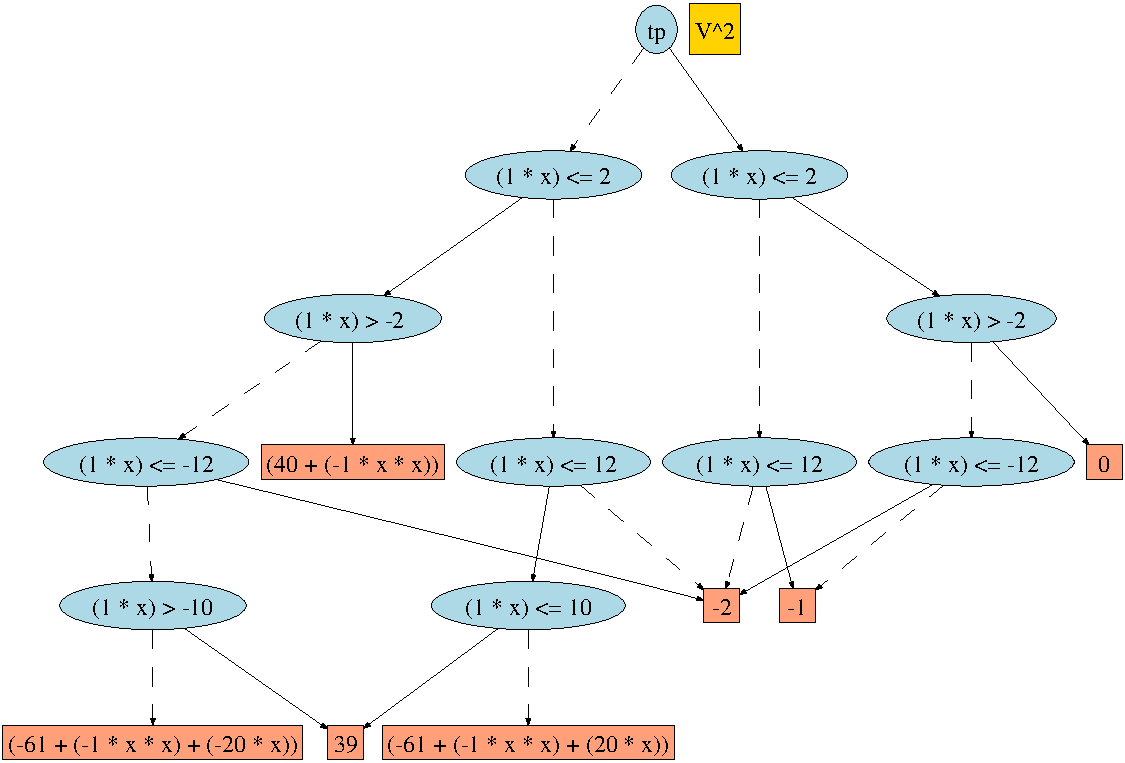
\includegraphics[width=0.8\textwidth]{pics/roverdot.pdf}
\vspace{6mm}

\caption{Optimal value function $V^2(x)$ for the
\textsc{Continuous Action}  \MarsRover\ problem represented as an (XADD) equal to the second diagram on the left. 
To evaluate
$V^2(x)$ for any state $x$, one simply traverses the diagram in a
decision-tree like fashion until a leaf is reached where the
non-parenthetical expression provides the \emph{optimal value} and the
parenthetical expression provides the \emph{optimal policy} 
($y = \pi^{*,2}(x)$) to achieve value $V^2(x)$.}
\label{fig:opt_val_pol}
\vspace{-5mm}
%\end{minipage}
%\vspace{-5mm}
\end{figure}
%%%%%%%%%%%%%%%%%%%%%%%%%%%%%%%%%%%%%%%%%%%%%%%%%%%%%%%%%%%%%%%%%%%%%%%%%%
The maximum long-term \emph{value} $V$ from a given state in \MarsRover\ 
is defined as a function of state variables:
{\footnotesize
%\begin{tabular}{l}
%$
% OBS: We do not know what is the problem related to the value function V. It certainty does not correspond to the previous problem definition. 


\begin{align*}
V = \begin{cases}
\neg \mathit{take\-pic}_1 \land \mathit{take\-pic}_2 \land (4 -x^2 -y^2\geq 0) \land 
(5 - x^2 - y^2\geq 0) : & 4 -x^2 -y^2 \\
\mathit{take\-pic}_1 \land \neg \mathit{take\-pic}_2 \land (2 -x^2 -y^2\geq 0) \land 
(3 - x^2 - y^2\geq 0) : & 2 -x^2 -y^2 \\
\neg \mathit{take\-pic}_1 \land \mathit{take\-pic}_2 \land (4 -x^2 -y^2\geq 0) \land 
(5 - x^2 - y^2\leq 0) : & -1 \\
\mathit{take\-pic}_1 \land \neg \mathit{take\-pic}_2 \land (2 -x^2 -y^2\geq 0) \land 
(3 - x^2 - y^2\leq 0) : & -1 \\
else &: 0 \\
\end{cases} 
%$
%\end{tabular}
\end{align*}
}
The value function is piecewise and non-linear, and contains non-rectangular decision
boundaries like $4 -x^2 -y^2\geq 0$. Figure~\ref{fig:opt_graph} presents the  0-step, 1-step, and 2-step time horizon solution for this problem. Despite the intuitive and simple nature of this result, we are unaware of prior methods that can produce such exact solutions. 

\paragraph{\WaterReservoir} 
Reservoir management is well-studied in
the OR literature \cite{Mahootchi2009,Yeh1985}.  The key continuous decision is how
much elapsed time $e$ to
\emph{drain} (or \emph{not drain}) each reservoir to maximize
electricity revenue over the decision-stage horizon while avoiding
reservoir overflow and underflow.  Cast as a CA-HMDP, we 
believe SVI provides the first approach capable of deriving
an exact closed-form non-myopic optimal policy
for all levels.

We examine a 2-reservoir problem with
respective levels $(l_1,l_2)\in [0,\infty]^2$ with reward penalties for 
overflow and underflow and a reward gain linear in the elapsed time $e$ for
electricity generated in periods when the $\mathit{drain}(e)$ action
drains water from $l_2$ to $l_1$ (the other action is 
$\mathit{no}$-$\mathit{drain}(e)$); we assume deterministic rainfall
replenishment and present the reward function as:  

\vspace{-4mm}
{\footnotesize
\begin{align*}
R & = \begin{cases}
((50-200*e) \leq l_1 \leq (4500-200*e)) \wedge ((50+100*e) \leq l_2 \leq (4500+100*e)) %\\ \hspace{4mm} \vspace{3mm} 
&:e\\
((50+300*e) \leq l_1 \leq (4500+300*e)) \wedge ((50-400*e) \leq l_2 \leq (4500-400*e)) %\\ \hspace{4mm} \vspace{3mm} 
&:0\\
\text{\normalsize otherwise} &: -\infty \\
\end{cases}
\end{align*}}
The transition function for levels of the $\mathit{drain}$ action is defined below. Note that for the $\mathit{no}$-$\mathit{drain}$ action, the $\mathit{500 * e}$ term is not involved.
{%\footnotesize 
\begin{align*}
l_1' & =(400 * e + l_1 -700 * e + 500 * e) \\
l_2'& =(400 * e + l_2 - 500 * e) \\
\end{align*}}

Similar to the discrete version of the \InventoryControl problem in the introduction, the DA-HMDP setting for these two problems defines discrete actions by partitioning the action space of each domain into $i$ number of slices. For example the \MarsRover\ problem with 2 actions which are the lower and upper bounds on $a$ ($a_1=-10, a_2 = 10$) and the transition and reward functions are defined according to these constant values.
We now provide the empirical results obtained from implementing our algorithms.

\subsection{Results}

For both the \textsc{Discrete Action} and \textsc{Continuous Action} \MarsRover\ domains, 
we have run experiments to evaluate our SDP solution 
in terms of time and space cost while varying the horizon and problem size.

%%%%%%%%%%%%%%%%%%%%%%%%%%%%%%%%%%%%%%%%%%%%%%%%%%%%%%%%%%%%%%%%%%%%%%%%%%
\begin{figure*}[t]
\centering
%\subfigure{
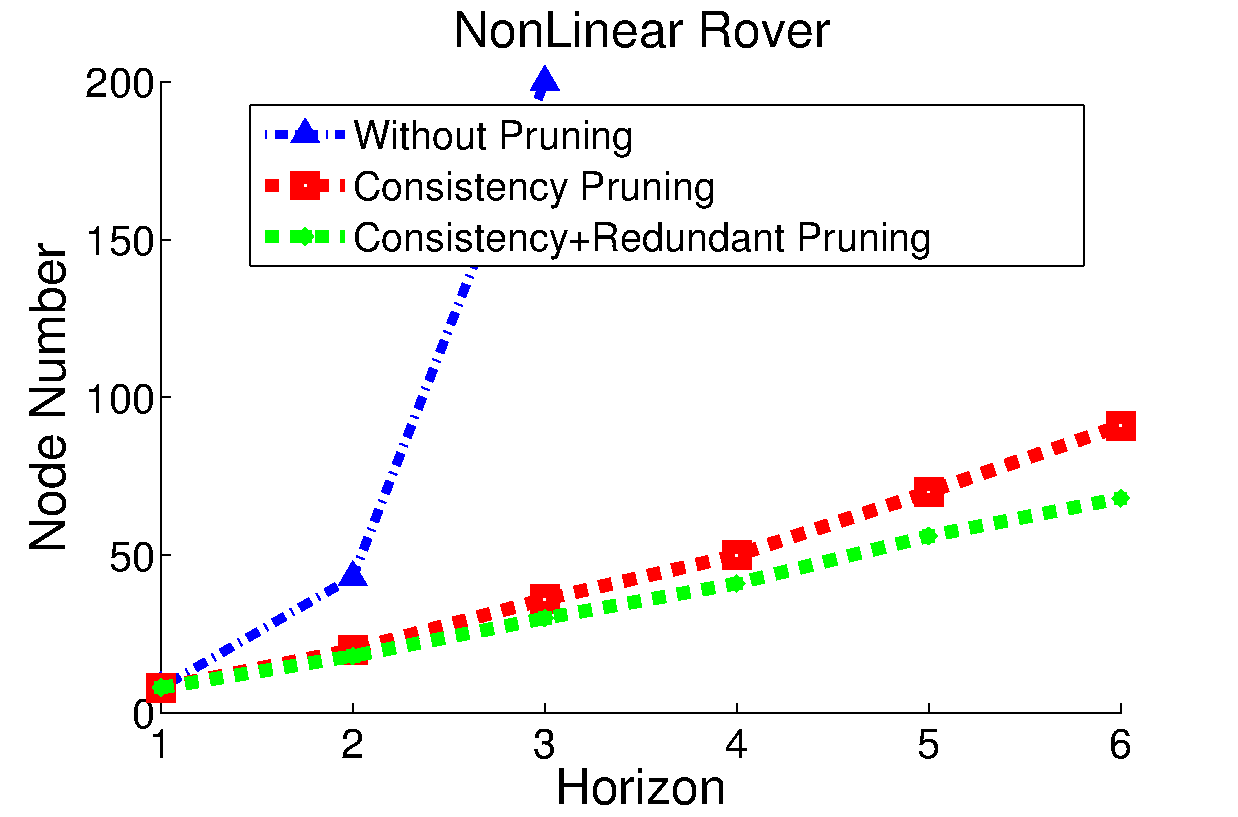
\includegraphics[width=0.45\textwidth]{pics/contRoverNode2.pdf}
%\hspace{5mm}
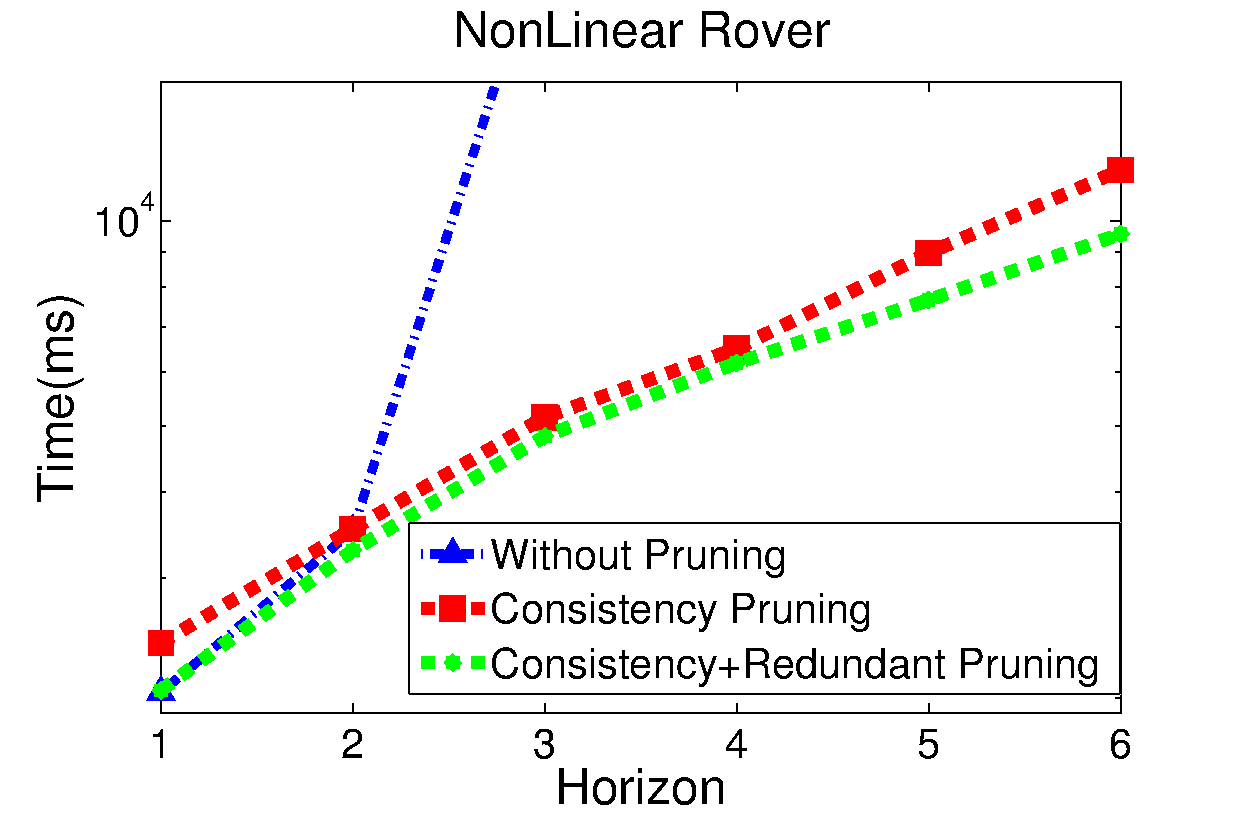
\includegraphics[width=0.45\textwidth]{pics/contRoverTime2.pdf}
%}
\vspace{-3mm}
\caption{%\footnotesize 
Space (\# XADD nodes in value function) and
time for different iterations (horizons) of SDP on quadratic \textsc{Continuous Action}  \MarsRover\ with 4 different results based on pruning techniques. Results are shown for  the XADD 
 with no pruning technique, with only consistency checking (using LP-solver) and with both the consistency and redundancy checking with a numerical precision heuristic.} %does it need more explaining? 
\label{fig:roverTS}
\end{figure*}
%%%%%%%%%%%%%%%%%%%%%%%%%%%%%%%%%%%%%%%%%%%%%%%%%%%%%%%%%%%%%%%%%%%%%%%%%%

%%%%%%%%%%%%%%%%%%%%%%%%%%%%%%%%%%%%%%%%%%%%%%%%%%%%%%%%%%%%%%%%%%%%%%%%%%
%figure5 : time-iteration and space-iteraton for 1d-2d-noPrune inventory
\begin{figure}[tbp!]
\vspace{2mm}
\centering
%\subfigure{
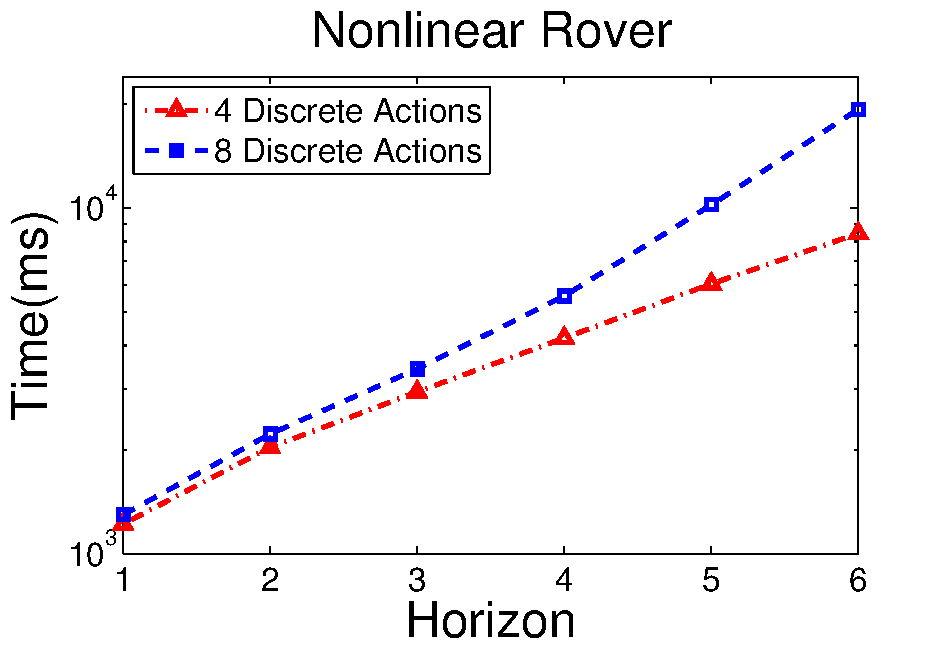
\includegraphics[width=0.45\textwidth]{pics/DisRoverNode.pdf}
\hspace{2mm}
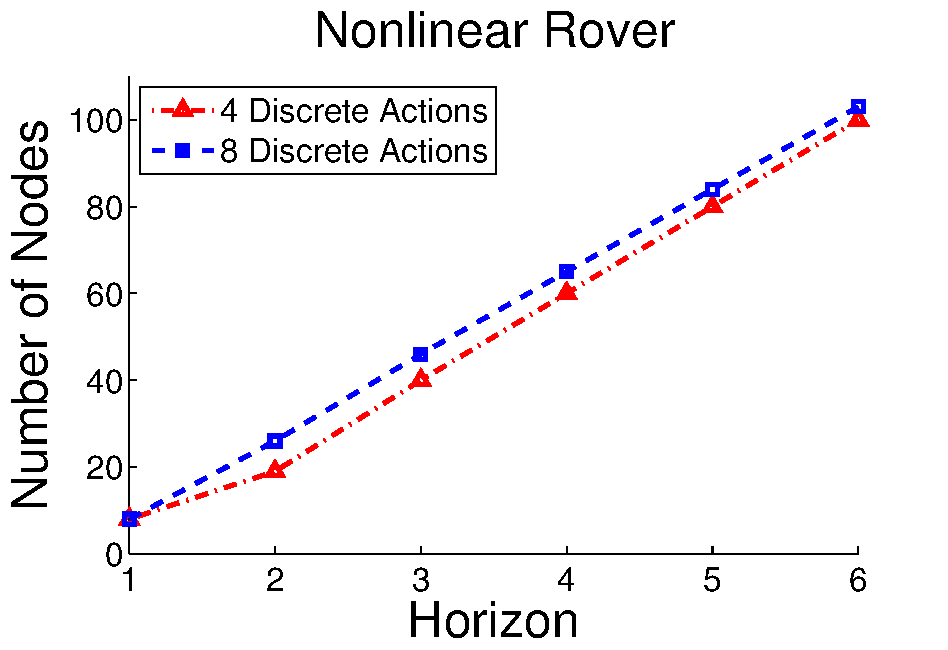
\includegraphics[width=0.45\textwidth]{pics/DisRoverTime.pdf}
%}
\vspace{-2mm}
\caption{%\footnotesize 
Space and elapsed time vs. horizon for a fixed discretization of 4 and 8 for the \MarsRover domain. This demonstrates how the number of nodes and time increases for each horizon. 
}
\label{fig:roverDisTS}
\vspace{-1mm}
\end{figure}
%%%%%%%%%%%%%%%%%%%%%%%%%%%%%%%%%%%%%%%%%%%%%%%%%%%%%%%%%%%%%%%%%%%%%%%%%%

For the \textsc{Continuous Action} \MarsRover problem, we present the time and space analysis in Figure~\ref{fig:roverTS}. Here three evaluations are performed based on the pruning algorithms of Section~\ref{sec:pruningAlg}. We note that without the inconsistency checking of Algorithm~\ref{algPrune}, SDP can not go beyond the third iteration as it produces many inconsistent nodes. The comparison is performed with consistency pruning and redundancy checking. The full pruning experiment also uses a numerical heuristic that omits similar branches. %With the full pruning of Algorithm~\ref{algRedundant} less than 10 \% node reduction is achieved but due to the calls made to the SAT-Solver the time increases to more than 10 times of that of the heuristic pruning. 
However even with the heuristic approach very little node reduction can be gained from redundancy pruning. This suggests that in some domains using redundancy pruning in not efficient and should be omitted from the final results. 
Hence we will present results for the \WaterReservoir and \InventoryControl problem with only consistency pruning. 

Next we present the analysis of the \textsc{Discrete Action} \MarsRover\ domains. Figure~\ref{fig:roverDisTS} shows how time and space costs of different horizons increases for a fixed action discretization of 4 and 8.
Note that one of the caveats of using a discrete setting is defining the actual discrete actions. In the continuous setting an action is defined between a large high and low range (e.g $a \in$ [$-1000000,1000000$]) allowing the SDP algorithm to choose the best possible action among all the answers. However for a discrete setting, choosing the range to discretize the action becomes very important. As an example in the rover description, allowing actions to be far from the center (e.g. $a \in$ [$-20,20$]) does not result in a converged solution. Finding this range is one of the drawbacks of using a discrete setting. 
%%%%%%%%%%%%%%%%%%%%%%%%%%%%%%%%%%%%%%%%%%%%%%%%%%%%%%%%%%%%%%%%%%%%%%%%%%
%OBS: The title in these figures must be "action" instead of "iteration".

%figure5 : time-iteration and space-iteraton for 1d-2d-noPrune inventory
\begin{figure}[tbp!]
\vspace{-2mm}
\centering
%\subfigure{
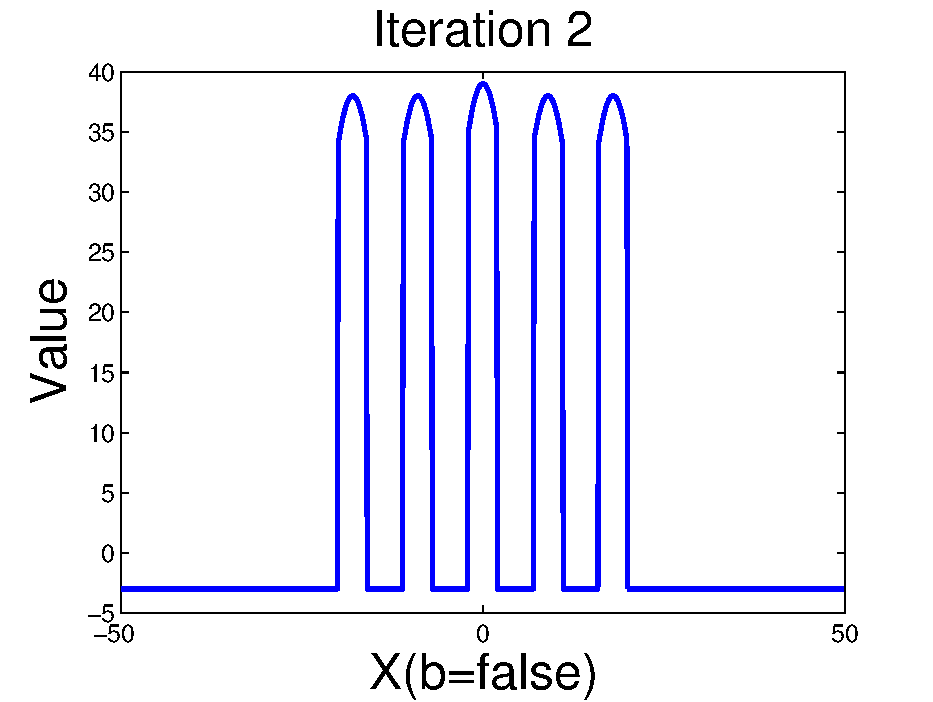
\includegraphics[width=0.18\textwidth]{pics/rover2.pdf}
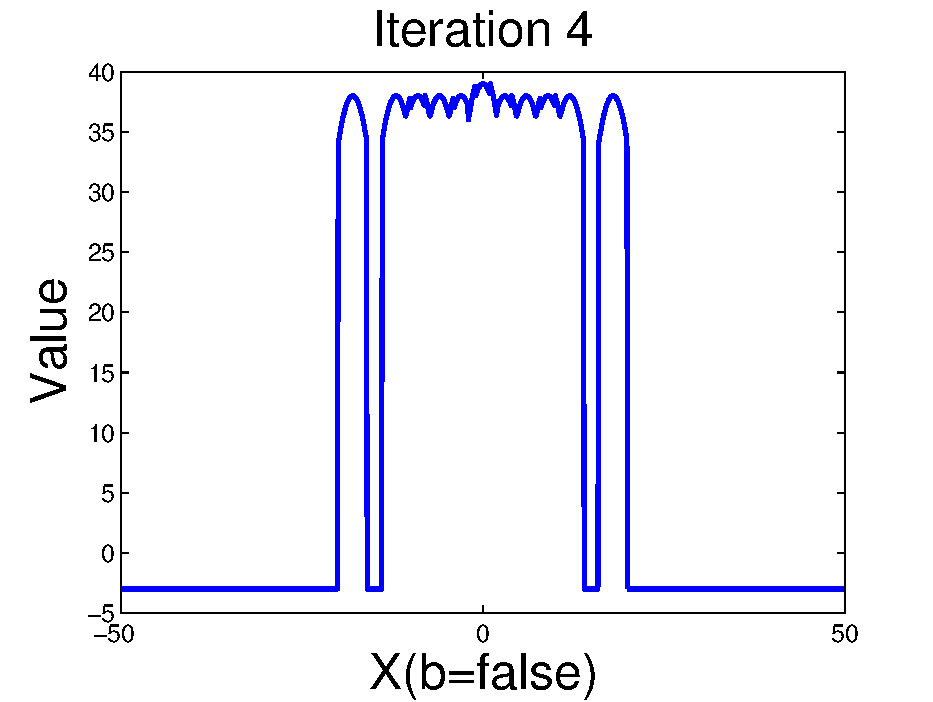
\includegraphics[width=0.18\textwidth]{pics/rover4.pdf}
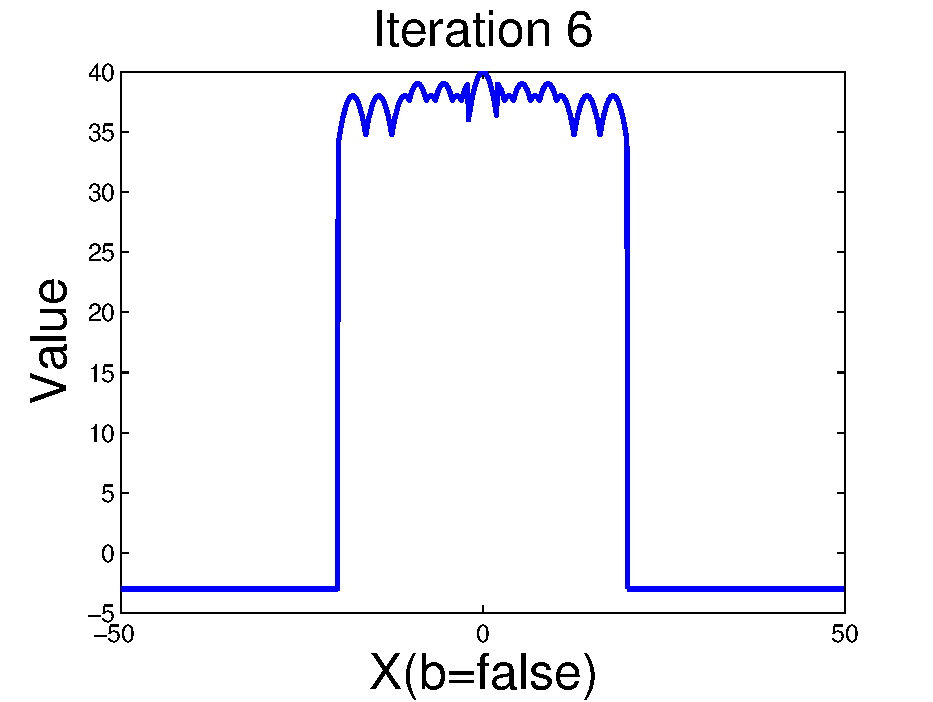
\includegraphics[width=0.18\textwidth]{pics/rover6.pdf}
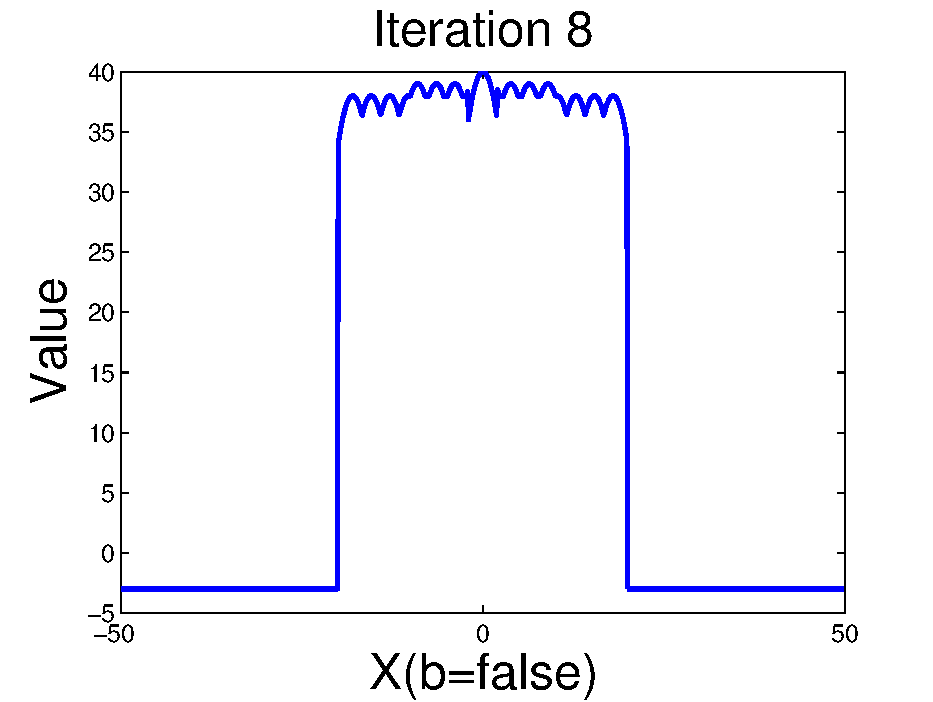
\includegraphics[width=0.18\textwidth]{pics/rover8.pdf}
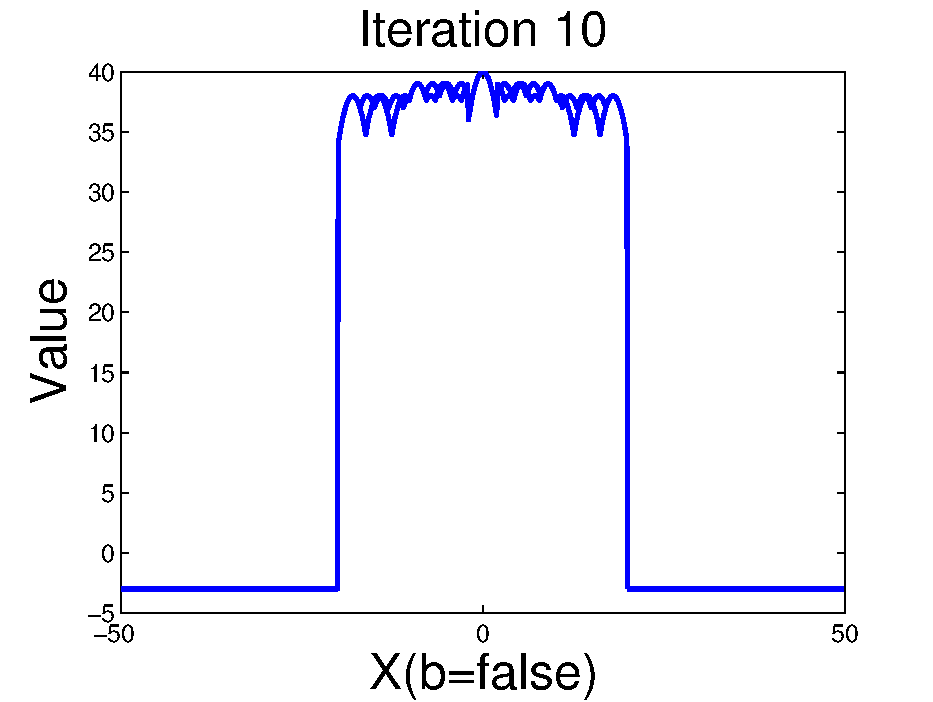
\includegraphics[width=0.18\textwidth]{pics/rover10.pdf}

%}
\vspace{-2mm}
\caption{%\footnotesize 
$V^3$ for different number of \textsc{Discrete Actions} in the \MarsRover\ problem. As the number of discrete actions increases, the value function more closely resembles the continuous action value of $V^2$ (defined in Figure ~\ref{fig:opt_val_pol}).
}
\label{fig:rover_discrete}
\vspace{-1mm}
\end{figure}
%%%%%%%%%%%%%%%%%%%%%%%%%%%%%%%%%%%%%%%%%%%%%%%%%%%%%%%%%%%%%%%%%%%%%%%%%%

On the other hand, the level of discretization within this range is also very important. To show this visually Figure~\ref{fig:rover_discrete} shows the results of the third iteration for 6 different discretizations compared to the continuous result. This figure proves the need to finely partition the action space within the predefined range. However as Figure~\ref{fig:roverDisSize} demonstrates, increasing the number of discrete action (for the fixed horizon of 3), leads to increasing time and space costs. Here results of different level of discretization is similar for the \WaterReservoir problem.

%%%%%%%%%%%%%%%%%%%%%%%%%%%%%%%%%%%%%%%%%%%%%%%%%%%%%%%%%%%%%%%%%%%%%%%%%%
%figure5 : time-iteration and space-iteraton for 1d-2d-noPrune inventory
\begin{figure}[tbp!]
\vspace{-2mm}
\centering
%\subfigure{
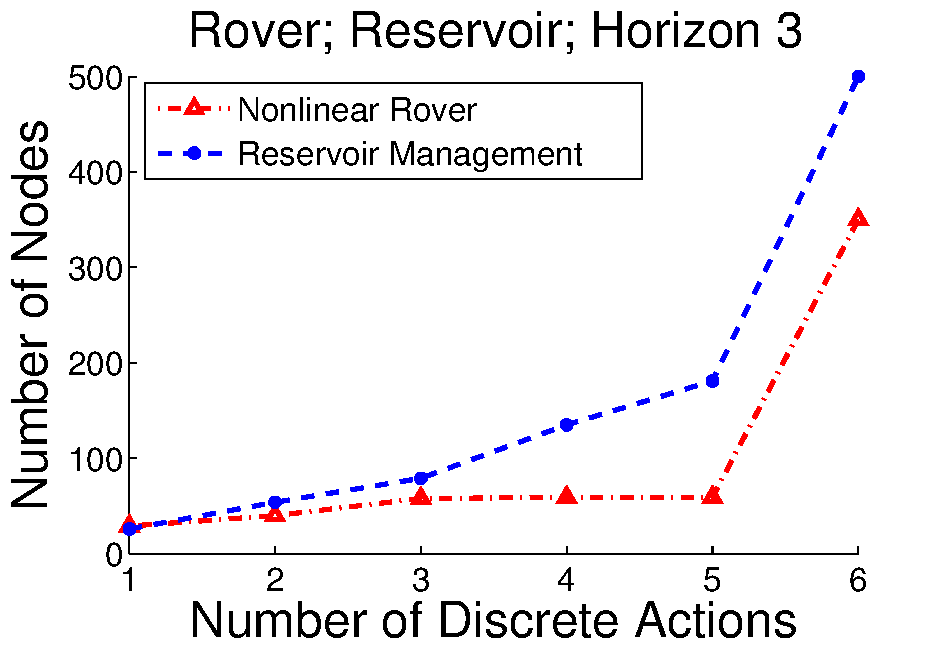
\includegraphics[width=0.45\textwidth]{pics/disRovResNode2.pdf}
\hspace{2mm}
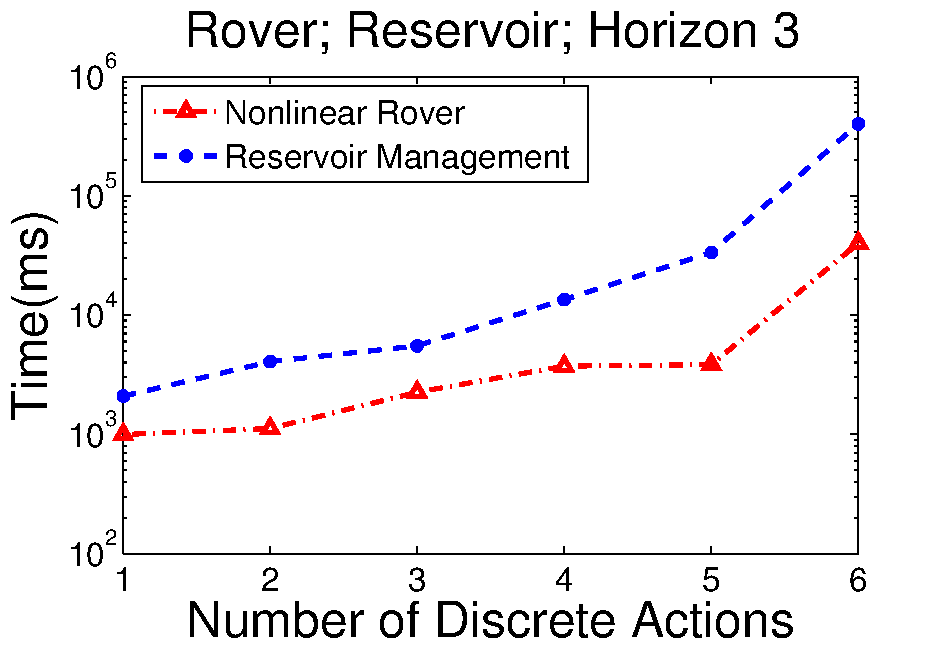
\includegraphics[width=0.45\textwidth]{pics/disRovResTime2.pdf}
%}
\vspace{-2mm}
\caption{%\footnotesize 
Space and elapsed time vs. number of discrete actions for a fixed horizon of 3  for  \MarsRover\ and the \WaterReservoir with discrete actions. 
}
\label{fig:roverDisSize}
\vspace{-5mm}
\end{figure}
%%%%%%%%%%%%%%%%%%%%%%%%%%%%%%%%%%%%%%%%%%%%%%%%%%%%%%%%%%%%%%%%%%%%%%%%%%

%%%%%%%%%%%%%%%%%%%%%%%%%%%%%%%%%%%%%%%%%%%%%%%%%%%%%%%%%%%%%%%%%%%%%%%%%%
%figure5 : time-iteration and space-iteraton for 1d-2d-noPrune inventory
\begin{figure}[tbp!]
\vspace{2mm}
\centering
%\subfigure{
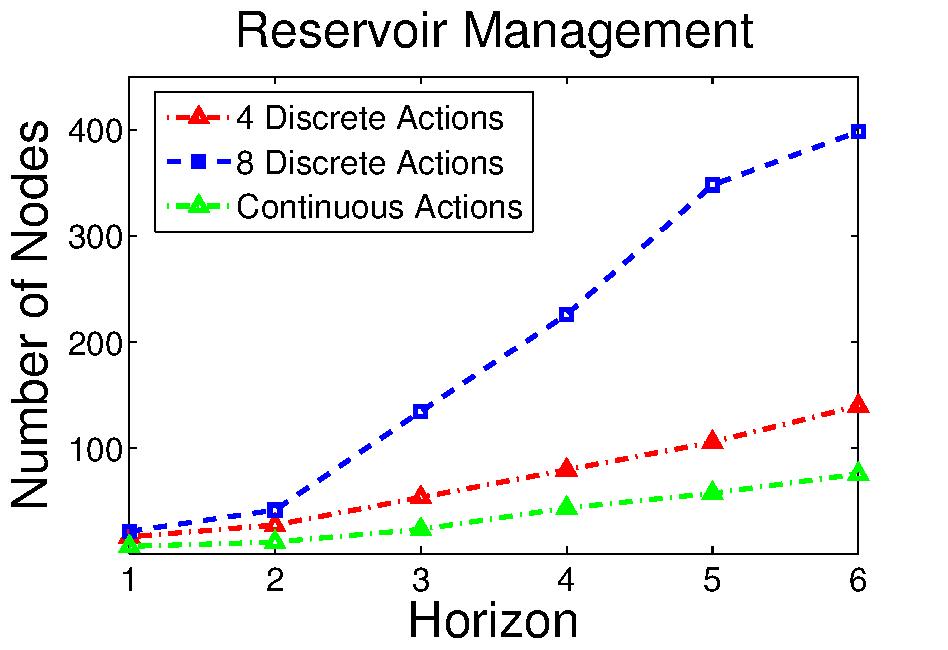
\includegraphics[width=0.45\textwidth]{pics/DisResNode2.pdf}
\hspace{2mm}
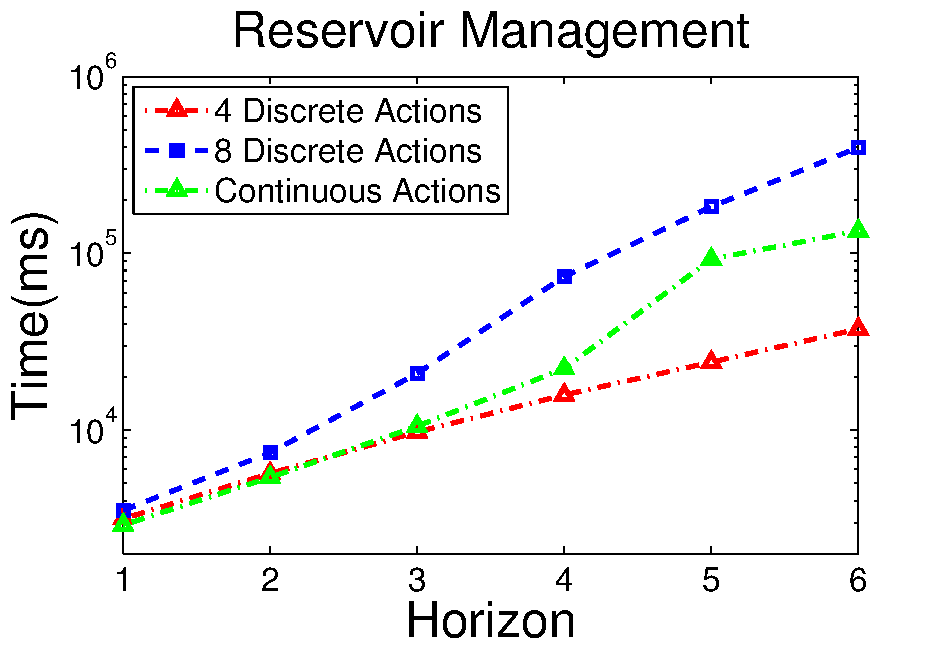
\includegraphics[width=0.45\textwidth]{pics/DisResTime2.pdf}
%}
\vspace{-2mm}
\caption{%\footnotesize 
Space and elapsed time vs. horizon for a fixed discretization of 4 and 8 actions for the \WaterReservoir.}
\label{fig:resDisTS}
\vspace{-5mm}
\end{figure}
%%%%%%%%%%%%%%%%%%%%%%%%%%%%%%%%%%%%%%%%%%%%%%%%%%%%%%%%%%%%%%%%%%%%%%%%%%

Figure~\ref{fig:resDisTS} presents the time and number of nodes for different horizons for 4 and 8 discrete actions compared to the continuous actions in the \WaterReservoir domain. Although in the first two iterations the time and space of the discrete action setting are similar, however for higher horizons more time and space is required in the 8 discrete action case. The number of nodes are lower for the continuous case compared to both discretizations but the time elapsed is higher than the 4-discrete actions due to the complexity of the continuous action maximization.

%%%%%%%%%%%%%%%%%%%%%%%%%%%%%%%%%%%%%%%%%%%%%%%%%%%%%%%%%%%%%%%%%%%%%%%%%%
\begin{figure*}[tbp!]
%\vspace{-1mm}
\centering
\vspace{10mm}
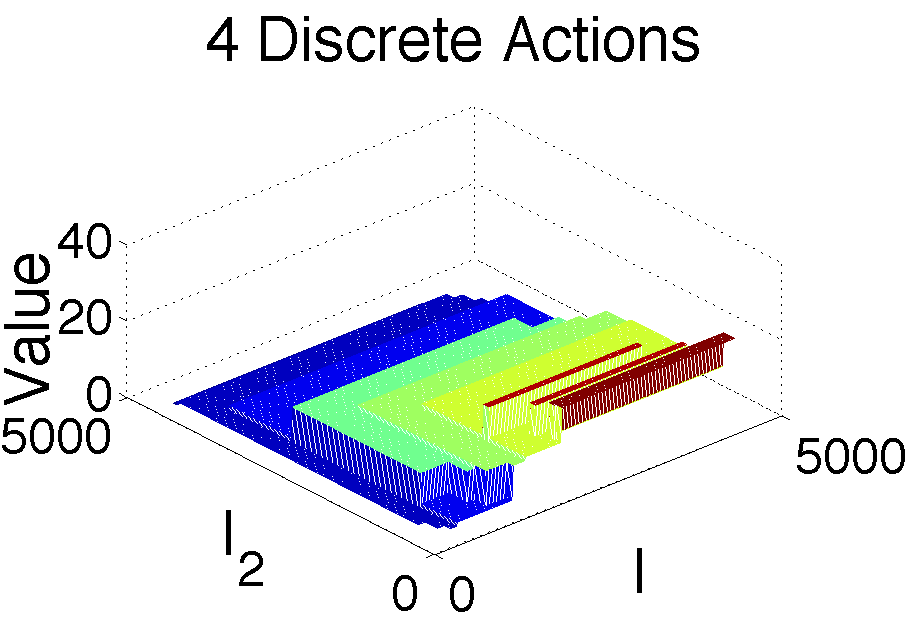
\includegraphics[width=0.48\textwidth]{pics/res3d4.pdf} 
\hspace{2mm}
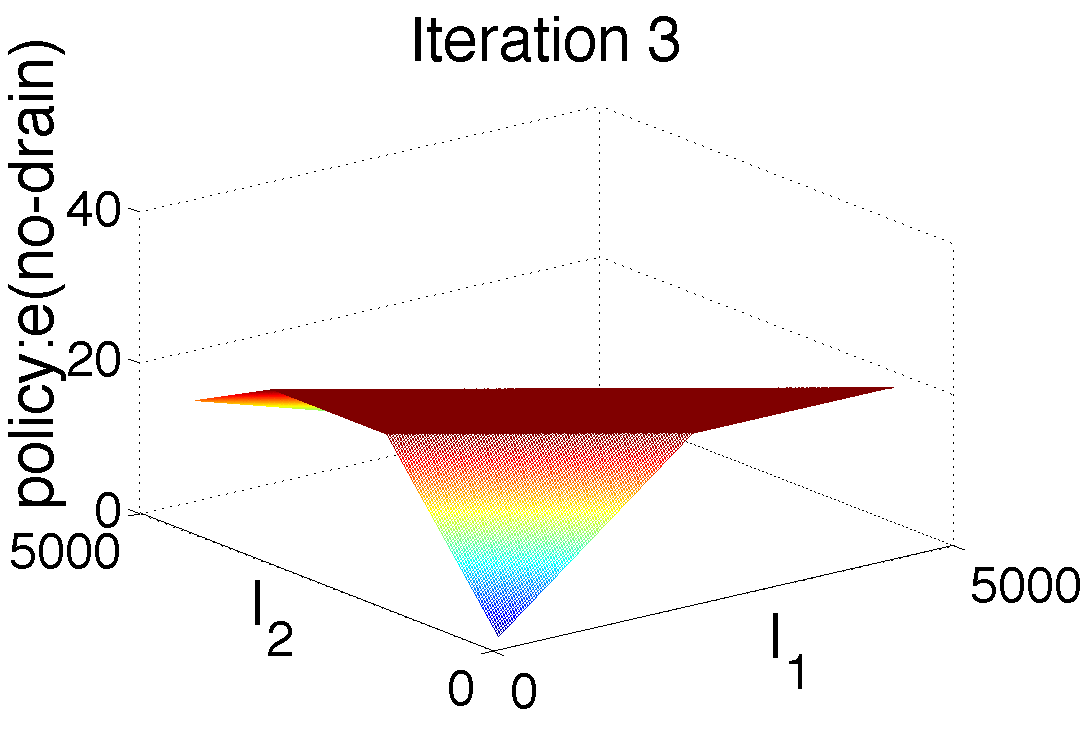
\includegraphics[width=0.48\textwidth]{pics/q3.pdf}
\vspace{10mm}
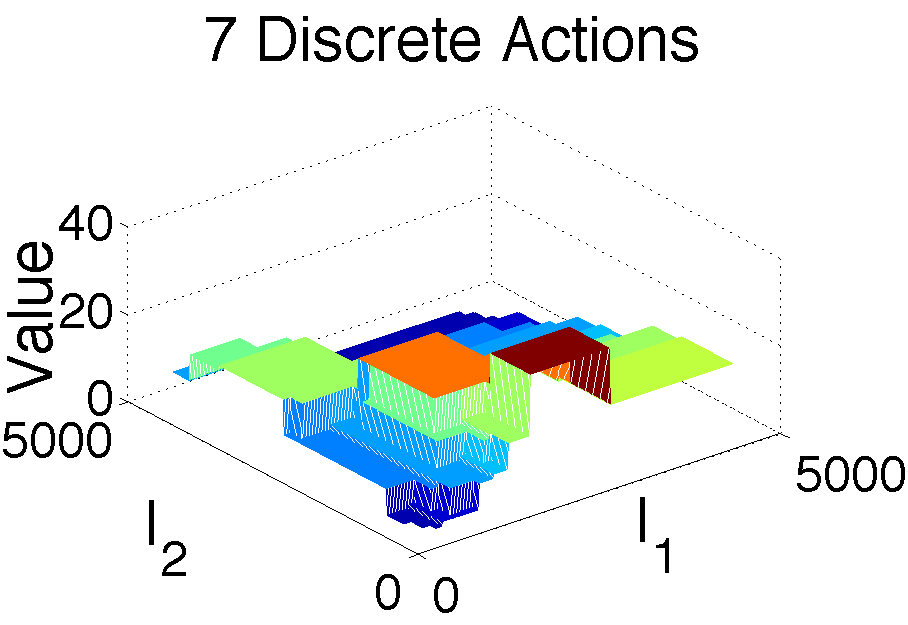
\includegraphics[width=0.48\textwidth]{pics/res3d7.pdf}
\hspace{2mm}
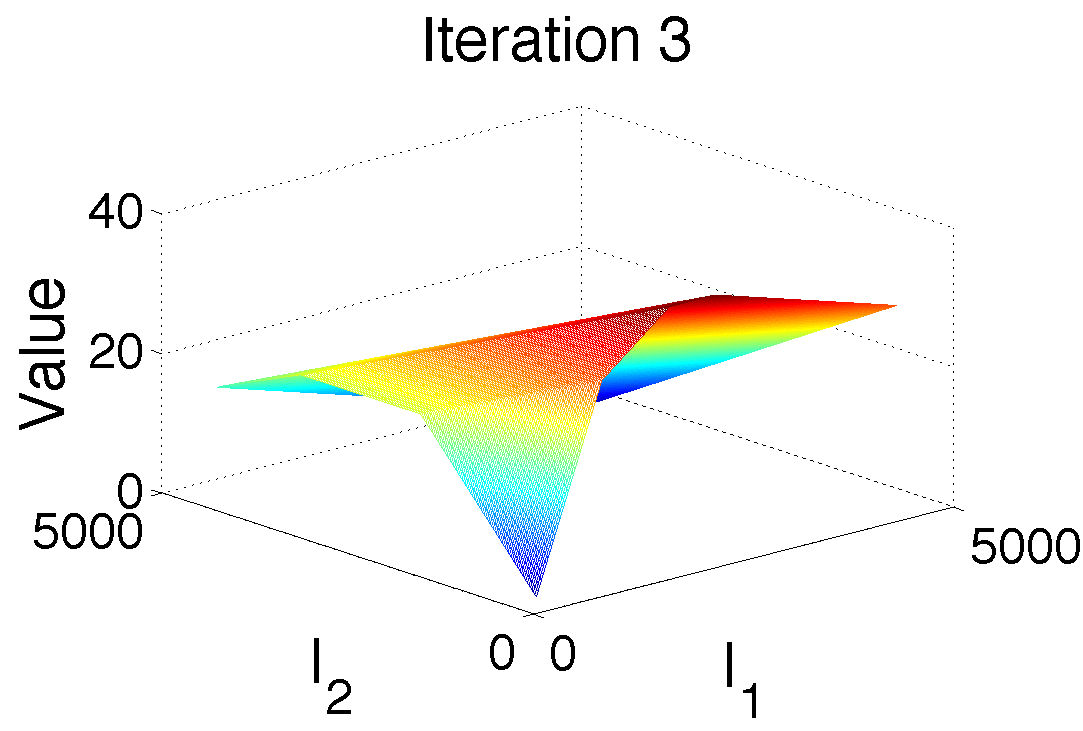
\includegraphics[width=0.48\textwidth]{pics/v3.pdf}
\vspace{10mm}
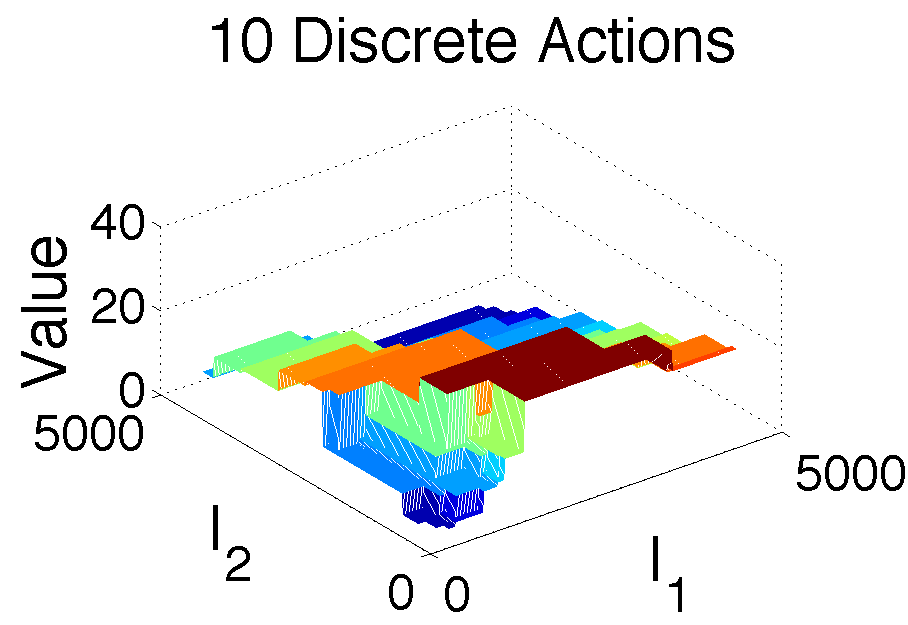
\includegraphics[width=0.48\textwidth]{pics/res3d10.pdf}
\hspace{2mm}
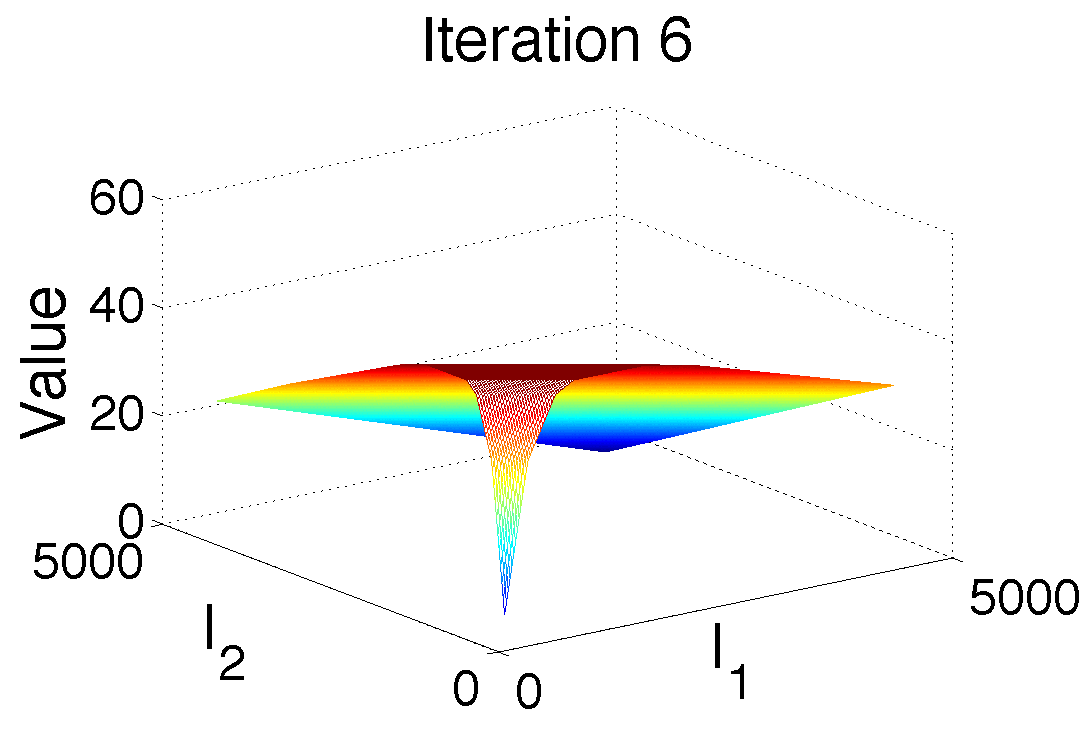
\includegraphics[width=0.48\textwidth]{pics/v6.pdf}
%\vspace{-3mm}
\caption{%\footnotesize 
Results for the \textsc{Discrete Action} and \textsc{Continuous Action} of the \WaterReservoir problem. {\it (left)} 4, 7 and 10 \textsc{Discrete Actions} of the \WaterReservoir problem for different water levels in iteration $V^3$. Each discretization draws the value closer to that of the continuous action \WaterReservoir on the right. {\it (right)} Policy $\mathit{no}$-$\mathit{drain}(e)=\pi^{3,*}(l_1,l_2)$ 
showing on the z-axis the elapsed time $e$ that should be executed 
for $\mathit{no}$-$\mathit{drain}$ conditioned on the states; followed by $V^3(l_1,l_2)$ and $V^6(l_1,l_2)$.
}
\label{fig:discreteplots}
%\vspace{-1mm}
\end{figure*}
%%%%%%%%%%%%%%%%%%%%%%%%%%%%%%%%%%%%%%%%%%%%%%%%%%%%%%%%%%%%%%%%%%%%%%%%%%
Figure~\ref{fig:discreteplots} (left) demonstrates three levels of discretization in the \WaterReservoir problem. The top left figure assumes 4 discrete actions, the middle figure has 7 actions and the bottom figure uses 10 discrete actions. The value of the third iteration is represented for all figures w.r.t. water levels $l_1$ and $l_2$. The figures suggest that finer grain discretization results in better results, closer to that of the continuous action value in middle right figure. 

Furthermore Figure~\ref{fig:discreteplots} (right) plots the  
the optimal closed-form policy at $h=3$: the solution interleaves $\mathit{drain}(e)$ and $\mathit{no}$-$\mathit{drain}(e)$ where even horizons are the latter.
Here we see that we avoid draining for the longest elapsed time $e$ 
when $l_2$ is low (wait for rain to replenish) and $l_1$ is high (draining
water into it could overflow it).  $V^3(l_1,l_2)$ and $V^6(l_1,l_2)$
show the progression of convergence from horizon $h=3$ to $h=6$ ---
low levels of $l_1$ and $l_2$ allow the system to generate electricity
for the longest total elapsed time over 6 decision stages. 

In Figure~\ref{fig:invC}, we provide a time and space analysis of
deterministic- and stochastic-demand (resp. DD and SD) variants of the
SCIC and MJCIC problem for up to three items (the same scale of
problems often studied in the OR literature); for each number of items
$n \in \{ 1,2,3 \}$ the state (inventory levels) is $\vec{x} \in
[0,\infty]^n$ and the action (reorder amounts) is $\vec{y} \in
[0,\infty]^n$.  Orders are made at one month intervals and we solve
for a horizon up to $h=6$ months.  
%Here we see that linear feasibility checking/pruning in the XADD is crucial -- we cannot solve beyond $h=2$ without it for 1 item!  
While solving for larger numbers of
items and SD (rather than DD) both increase time and space, 
the solutions quickly reach quiescence indicating structural
convergence.

Figure~\ref{fig:invD6} represents the time and space for the deterministic \textsc{Discrete Action} \InventoryControl for a discretization of 6 actions and different inventory items for up to $h=6$ horizons. While the number of items affects both time and space, even for 6 discrete actions the 3-item inventory will have exponential time and space for the second horizon onwards. The reason is behind the high dimensions, for a 3-item inventory of 6 discrete actions, a total of $6 \times 6 \times 6$ actions are required!
%%%%%%%%%%%%%%%%%%%%%%%%%%%%%%%%%%%%%%%%%%%%%%%%%%%%%%%%%%%%%%%%%%%%%%%%%%
%figure5 : time-iteration and space-iteraton for 1d-2d-noPrune inventory
\begin{figure}[tbp!]
\vspace{-2mm}
\centering
%\subfigure{
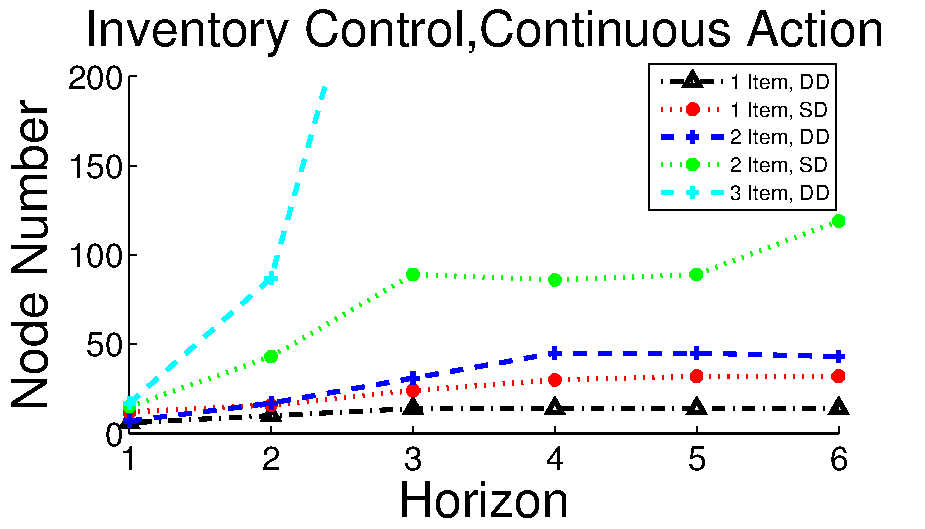
\includegraphics[width=0.45\textwidth]{pics/invCNode.pdf}
\hspace{2mm}
\includegraphics[width=0.45\textwidth]{pics/invCTime.pdf}
%}
\vspace{-2mm}
\caption{%\footnotesize 
\textsc{Continuous Action} \InventoryControl: space and time vs. horizon.
% comparing 
%1,2 or 3 States and actions (SA) with Deterministic (DD) 
%or Stochastic (SD) demand and no-pruning}.
}
\label{fig:invC}
\vspace{-2mm}
\end{figure}
%%%%%%%%%%%%%%%%%%%%%%%%%%%%%%%%%%%%%%%%%%%%%%%%%%%%%%%%%%%%%%%%%%%%%%%%%%
%%%%%%%%%%%%%%%%%%%%%%%%%%%%%%%%%%%%%%%%%%%%%%%%%%%%%%%%%%%%%%%%%%%%%%%%%%
%figure5 : time-iteration and space-iteraton for 1d-2d-noPrune inventory
\begin{figure}[tbp!]
\vspace{-2mm}
\centering
%\subfigure{
\includegraphics[width=0.45\textwidth]{pics/invD6Node.pdf}
\hspace{2mm}
\includegraphics[width=0.45\textwidth]{pics/invD6Time.pdf}
%}
\vspace{-2mm}
\caption{%\footnotesize 
\textsc{Discrete Action} \InventoryControl: Space and time vs. horizon for 6 discrete actions. Results are shown for various continuous items in the inventory.
% comparing 
%1,2 or 3 States and actions (SA) with Deterministic (DD) 
%or Stochastic (SD) demand and no-pruning}.
}
\label{fig:invD6}
\vspace{-2mm}
\end{figure}
%%%%%%%%%%%%%%%%%%%%%%%%%%%%%%%%%%%%%%%%%%%%%%%%%%%%%%%%%%%%%%%%%%%%%%%%%%
%%%%%%%%%%%%%%%%%%%%%%%%%%%%%%%%%%%%%%%%%%%%%%%%%%%%%%%%%%%%%%%%%%%%%%%%%%
%figure5 : time-iteration and space-iteraton for 1d-2d-noPrune inventory
\begin{figure}[tbp!]
\vspace{-2mm}
\centering
%\subfigure{
\includegraphics[width=0.45\textwidth]{pics/invH3Node.pdf}
\hspace{2mm}
\includegraphics[width=0.45\textwidth]{pics/invH3Time.pdf}
%}
\vspace{-2mm}
\caption{%\footnotesize 
Space and elapsed time vs. horizon for a fixed horizon of 3 and different problem sizes for the \textsc{Discrete Action} \InventoryControl. 
% comparing 
%1,2 or 3 States and actions (SA) with Deterministic (DD) 
%or Stochastic (SD) demand and no-pruning}.
}
\label{fig:invH3}
\vspace{-2mm}
\end{figure}
%%%%%%%%%%%%%%%%%%%%%%%%%%%%%%%%%%%%%%%%%%%%%%%%%%%%%%%%%%%%%%%%%%%%%%%%%%

Figure~\ref{fig:invH3} illustrates the effect of different number of action discretizations for the \InventoryControl. Time and space are presented for the fixed horizon of $h=3$ and for inventory items of $1,2$ and $3$. For a 1-item inventory, as the number of discrete actions increases, the time and space grows almost linearly. However for there is an exponential blow-up of the number of nodes for the 2-item inventory beyond 5 discrete actions while the time increases dramatically. Similar to the previous experiment, the 3-item inventory problem does not scale for more than two discrete actions due to the complexity in the action space. As a result of comparing the continuous and discrete action setting for the 2-item \InventoryControl problem, the advantage of the continuous action H-MDPs is obvious. 

Finally the key point evident in the results is the fact that scaling to higher dimensions requires large amounts of memory and time. This may be achievable using faster hardware, however a more efficient solution is to scale our XADD framework.

\section{Related Work}

The most relevant vein of related work for DA-HMDPs is that of \cite{feng04} and \cite{li05} which can perform exact dynamic programming on
HMDPs with rectangular piecewise linear reward and transition functions
that are delta functions.  While SDP can solve these same problems,
it removes both the rectangularity and piecewise restrictions on the
reward and value functions, while retaining exactness.  
Heuristic search approaches with formal guarantees 
like HAO* \cite{hao09} are an attractive future extension of SDP;
in fact HAO* currently uses the method of \cite{feng04}, which could
be directly replaced with SDP.  While \cite{penberthy94} has considered
general piecewise functions with linear boundaries (and in fact,
we borrow our linear pruning approach from this paper), this work
only applied to fully deterministic settings, not HMDPs.

Other work has analyzed limited HMDPS having only one continuous
state variable.  Clearly rectangular restrictions are meaningless with
only one continuous variable, so it is not surprising that more
progress has been made in this restricted setting.  One continuous
variable can be useful for optimal solutions to time-dependent MDPs 
(TMDPs) \cite{boyan01}.  Or phase transitions can be used to 
arbitrarily approximate one-dimensional continuous distributions
leading to a bounded approximation approach for arbitrary single continuous
variable HMDPs \cite{phase07}.  
While this work cannot handle arbitrary stochastic
noise in its continuous distribution, it does exactly solve HMDPs
with multiple continuous state dimensions.

There are a number of general HMDP approximation
approaches that use approximate linear programming \cite{kveton06}
or sampling in a reinforcement learning style approach \cite{munos02}.
In general, while approximation methods are quite promising in
practice for HMDPS, the objective of this paper was to push
the boundaries of \emph{exact} solutions; however, in some sense, 
we believe that more expressive exact solutions may also inform
better approximations, e.g., by allowing the use of data structures
with non-rectangular piecewise partitions that allow higher fidelity
approximations.

%As for continuous actions and states, there has been prior work on approximate solutions to continuous state MDPs \cite{munos02,phase07} and even continuous state and action
%MDPs \cite{kveton06}, which might inform future approximate extensions
%of this work.  
As for CA-HMDPs, there has been prior work in control theory. The field of linear-quadratic Gaussian (LQG) control \cite{lqgc} which use linear dynamics with continuous actions, Gaussian noise, and quadratic
reward is most closely related.  However, these exact solutions do
not extend to discrete and continuous systems with \emph{piecewise}
dynamics or reward.
%Perhaps the most practical extension
%for future work would to combine SDP with the initial state focused
%dynamic programming techniques \cite{hao09} to increase exact solution
%efficiency when the initial state is known.
%
%While it should be theoretically possible to relax some of the 
%constraints of our setting to nonlinear dynamics or more general
%nonlinear rewards, we have carefully chosen our restrictions 
%to ensure \emph{linear piecewise boundaries}, which permit the use
%of fast linear feasibility checkers (for XADD pruning) that has proved
%critical for efficiency in problems like \InventoryControl.  Hence we
%believe this work carefully balances the tradeoff between expressivity
%and computational efficiency.  
Combining this work with initial state focused techniques \cite{hao09}
and focused approximations that exploit optimal value
structure \cite{apricodd} or further
afield \cite{munos02,kveton06,phase07} are promising directions for
future work.
% more future work for continuous actions? 


\section{Concluding Remarks}

In this paper, we introduced a new symbolic approach to solving continuous problems in HMDPs exactly. In the case of discrete actions and continuous states, using arbitrary
reward functions and expressive nonlinear transition functions far exceeds the exact solutions possible with existing HMDP
solvers.  
As for continuous states and actions, a key contribution is that of \emph{symbolic constrained
optimization} to solve the continuous action maximization problem. We
believe this is the first work to propose optimal closed-form
solutions to MDPs with \emph{multivariate} continuous state \emph{and}
actions, discrete noise, \emph{piecewise} linear dynamics, and
\emph{piecewise} linear (or restricted \emph{piecewise} quadratic)
reward; further, we believe our experimental results are the first
exact solutions to these problems to provide a closed-form optimal
policy for all (continuous) states.

While our method is not scalable for 100's of items, it still represents
the first general exact solution methods for capacitated multi-inventory control problems. 
And although a linear or quadratic reward is quite limited but it has appeared useful for single continuous resource or continuous time problems such as the water reservoir problem. 

In an effort to make SDP practical, we also introduced
the novel XADD data structure for representing arbitrary piecewise
symbolic value functions and we addressed the complications that
SDP induces for XADDs, such as the need for reordering and pruning the decision
nodes after some operations.  All of these are substantial contributions
that have contributed to a new level of expressiveness for HMDPS
that can be exactly solved.

There are a number of avenues for future research.  First off, it is
important examine what generalizations of the transition function used
in this work would still permit closed-form exact solutions.  In terms
of better scalability, one avenue would explore the use of initial
state focused heuristic search-based value iteration like
HAO* \cite{hao09} that can be readily adapted to use SDP.  Another
avenue of research would be to adapt the lazy approximation approach
of \cite{li05} to approximate HMDP value functions as piecewise
linear XADDs with linear boundaries that may allow for better
approximations than current representations that rely on rectangular
piecewise functions.  Along the same lines, ideas from
APRICODD \cite{apricodd} for bounded approximation of discrete ADD
value functions by merging leaves could be generalized to XADDs.
Altogether the advances made by this work open up a number of
potential novel research paths that we believe may help make
rapid progress in the field of decision-theoretic planning
with discrete and continuous state.

With the current solution for continuous states and actions, we can apply our methods to real-world data from the Inventory literature with more exact transitions and rewards. Fully stochastic distributions are required for these problems which is a major future direction by in-cooperating a noise parameter in the models. 
Also we have looked into value iteration for both problems, solving the symbolic policy iteration algorithm for problems with simple policies can prove to be effective in certain domains. 
The other promising direction is to extend the current exact solution for non-linear functions and solving polynomial equations using computational geometric techniques. 

Verificar:

Note that, for arbitrary functions, finding a canonical  expression form may be time consuming or intractable.

Theoretically, this does not affect our solution but in practice if we have non linear decision nodes, we can't prune redundant nodes or inconsistency paths resulting in large XADDs.


\section*{Acknowledgements}

%\appendix

\vskip 0.2in
\bibliography{exactsdp}
\bibliographystyle{theapa}

\end{document}
